\documentclass[11pt,a4paper, twocolumn]{article}
\usepackage[utf8]{inputenc}
\usepackage{multirow}
\usepackage{amsmath}
\usepackage{bookmark}
\usepackage{graphicx}
\usepackage{hyperref}
\usepackage{algorithm}
\usepackage{algpseudocode}
\usepackage{booktabs}
\usepackage{multirow}
\usepackage{graphicx}
\usepackage{subcaption}
\usepackage{caption}
\usepackage{xcolor}

\title{Solving the Two and Three Body Problems with Deep Learning Models \\
  \large Machine Learning in Physics Course Exam}
\author{Julian Roddeman (s1080491)}
\date{\today}

\begin{document}

\twocolumn[
\begin{@twocolumnfalse}
  \maketitle
  \begin{abstract}
    This study addresses the two-body and three-body problems using deep learning models, with a focus on Physics-Informed Neural Networks (PINNs). This papers covers data generation for multiple orbital scenarios, implement and compare different neural network architectures (MLP, LSTM, and PINN), and evaluate their performance in predicting trajectories. The approach demonstrates the potential of machine learning techniques in predicting orbits and velocities, particularly highlighting the advantages of physics-informed methods. The codebase for this project is available on GitHub at \url{https://github.com/JulianRodd/Orbit_Prediction}. Appendix \ref{sec:repository} provides details about the repository structure and the README file in the root directory constains instructions for running the code.
    \end{abstract}
\end{@twocolumnfalse}
]
  \section{Introduction}
  \label{sec:introduction}
  The two-body and three-body problems are challenges in physics. This study explores the application of deep learning models to solve these problems. We begin by simulating two-body and three-body problems with varying initial conditions and increased acceleration and additional force scenarios. We then implement and compare different neural network architectures, including Multilayer Perceptron (MLP), Long Short-Term Memory (LSTM), and Physics-Informed Neural Networks (PINNs). Our evaluation focuses on model performance in predicting orbital trajectories for different time horizons, specifically 10, 100, and 500 steps. We analyze the advantages of incorporating physical constraints in neural networks through PINNs, aiming to improve prediction accuracy and physical consistency. By comparing the performance of these models across the various scenarios, we aim to provide insights into the strengths and limitations of different deep learning approaches in solving gravitational problems.

\section{Literature Review}
\label{sec:literature}

Neural networks have shown promise in orbital mechanics, with Liao et al. \cite{liao2020} successfully applying them to find and classify periodic orbits in the three-body problem. The introduction of Physics-Informed Neural Networks (PINNs) by Raissi et al. \cite{raissi2019} has further advanced the field, offering a framework to incorporate physical laws directly into neural network architectures. In the context of gravitational problems, Martin and Schaub \cite{martin2022} demonstrated PINNs' efficacy in modeling gravity fields of celestial bodies.

Deep learning approaches have also been applied to related challenges in astrodynamics. Cheng et al. \cite{cheng2020} utilized neural networks for real-time optimal control in asteroid landings, while Gao and Liao \cite{gao2019} proposed an efficient gravity field modeling method based on Gaussian process regression. These advancements highlight the potential of machine learning in addressing complex gravitational dynamics.

However, challenges persist in ensuring physical constraints are properly enforced, avoiding overfitting, and generalizing to new scenarios. The physics-informed approach partially addresses these issues, but further research is needed to optimize network architectures, incorporate more comprehensive physical knowledge, and extend these methods to more complex N-body scenarios \cite{meng2022physics}. This literature review sets the stage for our study, which aims to contribute to this evolving field by exploring the application of neural networks and PINNs to two-body and three-body gravitational problems.
\section{Methodology}
\label{sec:methodology}
\subsection{Data Generation}
Our data generation process was designed to create diverse, realistic orbital scenarios for two-body and three-body gravitational problems, while incorporating measurement uncertainties to reflect real-world challenges. We implemented three main simulation scenarios: the standard two-body problem, a two-body problem with increased acceleration, and a three-body problem.
For the two-body problem, we simulated the motion of a light rotating object (spaceship) around a very heavy stationary object. The initial radius was set to 10,000 m, with the initial velocity calculated to achieve a stable circular orbit. In the increased acceleration scenario, we introduced an additional sinusoidal force on the spaceship, simulating a propulsion system malfunction.
The three-body problem involved simulating the motion of a light object (spaceship) under the gravitational influence of two heavy bodies. We generated varied initial conditions by randomizing the initial position and velocity of the spaceship within reasonable bounds.
All simulations were based on Newton's law of gravitation:
$$F = -G \frac{M m}{r^2} \hat{r}$$
where $G$ is the gravitational constant, $M$ and $m$ are the masses of the objects, $r$ is the distance between them, and $\hat{r}$ is the unit vector in the direction of $r$.
We used the Euler method for numerical integration to update the position and velocity of the objects:
\[v(t + \Delta t) = v(t) + a(t) \Delta t\]
\[r(t + \Delta t) = r(t) + v(t)\Delta t\]
To reflect real-world measurement challenges, we introduced a 1\% relative uncertainty to the angle, radius, and velocity measurements of the orbiting object. These uncertainties were implemented using Gaussian noise, clipped to ensure the relative error remains within ±1\%.
For each scenario, we simulated a total of 10 trajectories (spaceships) with different initial conditions, each for 100,000 time steps. We implemented rigorous checks to ensure the generated orbits are valid and realistic. For the two-body problem, we verified that the trajectory forms at least one complete orbit, spans a significant range in both x and y directions, and doesn't simply fly away. For the three-body problem, we additionally checked that the trajectory is bounded, shows sufficient complexity, and remains within a reasonable distance from the center of the system.
The data was split into training, validation, and test sets. Nine spaceships were used for training and validation, with their trajectories divided into sequences and split using 5-fold cross-validation. One spaceship was reserved exclusively for the test set, providing a truly unseen trajectory for final model evaluation.
To verify the quality of our generated data, we implemented visualization functions to plot the trajectories and velocities for each scenario. These visualizations helped ensure the simulated orbits were realistic and exhibited the expected behaviors for each problem type.
This comprehensive data generation approach provides a robust foundation for training and evaluating machine learning models on orbital mechanics problems, addressing the key requirements of simulating realistic scenarios with varying complexity and uncertainty levels.
\subsection{Model Architectures}

To address the challenge of predicting orbital dynamics, we implemented and compared three neural network architectures: Multilayer Perceptron (MLP), Long Short-Term Memory (LSTM), and Physics-Informed Neural Network (PINN). Each architecture was designed to capture different aspects of the two-body and three-body problems, including scenarios with increased acceleration.

\begin{table}[h]
  \centering
  \scriptsize
  \caption{Overview of Model Architectures}
  \label{tab:model-architectures}
  \begin{tabular}{@llll@{}}
  \toprule
  \textbf{Feature} & \textbf{MLP} & \textbf{LSTM} & \textbf{PINN} \\
  \midrule
  Input Size & 12 & 12 & 12 \\
  Hidden Layers & 3 & 2 & 4 \\
  Hidden Size & 256 & 128 & 256 \\
  Output Size & 4 & 4 & 4 \\
  Activation & LeakyReLU & ReLU & Tanh \\
  Dropout Rate & 0.2 & 0.2 & 0.1 \\
  Normalization & Batch & Layer & Batch \\
  Residual Conn. & Yes & Yes & Yes \\
  \bottomrule
  \end{tabular}
  \end{table}

The MLP serves as our baseline model, capable of learning non-linear relationships between input features and output predictions. Its architecture includes three hidden layers with 256 neurons each, using LeakyReLU activation and batch normalization.

The LSTM architecture, designed to capture temporal dependencies, utilizes a bidirectional LSTM layer with 128 hidden units and 2 layers. This is followed by two fully connected layers, each with 128 neurons and ReLU activation. Layer normalization is applied after the LSTM layer to stabilize training.

The PINN architecture incorporates physical constraints into the learning process. It consists of four hidden layers with 256 neurons each, using Tanh activation and batch normalization. Crucially, it employs a custom loss function that combines mean squared error with physics-based constraints:

\begin{equation}
_{total} = L_{MSE} + \lambda(L_{energy} + L_{momentum})
\end{equation}

Where $L_{MSE}$ is the standard mean squared error, $L_{energy}$ ensures conservation of total energy (kinetic + potential), and $L_{momentum}$ enforces conservation of linear momentum. The hyperparameter $\lambda$ balances the influence of physical constraints.

All models use residual connections and dropout to facilitate training of deeper networks and prevent overfitting. They were trained using the Adam optimizer with a learning rate of 0.001 and early stopping (patience of 5 epochs). We employed 5-fold cross-validation to ensure robust evaluation of each model's performance.

The selection of these architectures was motivated by their unique strengths. The Multilayer Perceptron (MLP) provides a simple yet effective baseline for comparison, offering a straightforward approach to learning complex patterns. The Long Short-Term Memory (LSTM) network excels in capturing long-term dependencies in orbital trajectories, making it particularly suitable for time-series prediction tasks. The Physics-Informed Neural Network (PINN) incorporates domain-specific knowledge, potentially leading to more physically plausible predictions by integrating fundamental physical laws into the learning process. By comparing these diverse approaches, we aim to determine the most effective method for predicting orbital dynamics across various scenarios and time horizons. This comparison allows us to balance between purely data-driven learning and physics-informed modeling, providing insights into the strengths and limitations of each approach in the context of celestial mechanics.

\subsubsection{Training Configuration}
We implemented a consistent training approach across all model architectures to ensure a fair comparison. The Adam optimizer was used with a learning rate of 0.001. For MLP and LSTM models, we employed Mean Squared Error (MSE) as the loss function, while PINN utilized a custom loss function (detailed elsewhere). All models were trained with a batch size of 32 for a maximum of 20 epochs, with early stopping implemented using a patience of 5 epochs. To ensure robust evaluation, we employed 5-fold cross-validation. Training was conducted for each model type (MLP, LSTM, PINN) on three dataset types: the two-body problem, the two-body problem with increased acceleration, and the three-body problem. In each training iteration, one fold was reserved for validation, allowing us to assess model performance on unseen data throughout the training process. This comprehensive approach allowed us to rigorously compare the performance of different model architectures across various gravitational scenarios while minimizing the risk of overfitting.

The \texttt{generic\_train} function in our codebase handles the training loop, implementing early stopping and model checkpointing. Training progress and performance metrics were logged using Weights \& Biases (wandb) for comprehensive experiment tracking.
\subsubsection{Physics-Informed Neural Networks}
The PINN architecture incorporates physical laws into the learning process through a custom loss function:
\begin{equation}
L_{\text{total}} = L_{\text{MSE}} + 0.1 \cdot (L_{\text{energy}} + L_{\text{momentum}})
\end{equation}
In this equation, $L_{\text{MSE}}$ represents the standard mean squared error between predicted and true values. $L_{\text{energy}}$ enforces energy conservation and is defined as:
\begin{equation}
L_{\text{energy}} = \frac{1}{N} \sum_{i=1}^N (E_{\text{pred},i} - E_{\text{true},i})^2
\end{equation}
where $E = \frac{1}{2}v^2 - \frac{GM_1}{r}$. Here, $v$ is velocity, $G$ is the gravitational constant, $M_1$ is the mass of the central body, and $r$ is the distance from the central body.
The $L_{\text{momentum}}$ term ensures momentum conservation:
\begin{equation}
L_{\text{momentum}} = \frac{1}{N} \sum_{i=1}^N (p_{\text{pred},i} - p_{\text{true},i})^2
\end{equation}
with $p = mv$ representing momentum.
This loss function is implemented in the \texttt{pinn\_loss} function, utilizing PyTorch's automatic differentiation capabilities. The physics-based terms are weighted by a factor of 0.1 to balance their influence with the data-driven MSE loss.
By incorporating these physics-based constraints, the PINN architecture aims to learn solutions that not only fit the data but also respect the underlying physical principles of orbital mechanics. This approach directly addresses the assignment's focus on PINNs and their potential advantages in solving gravitational problems, particularly for complex scenarios like the three-body problem and cases with increased acceleration.
Our implementation allows for a comprehensive comparison between purely data-driven approaches (MLP and LSTM) and the physics-informed method (PINN) across different orbital dynamics scenarios, providing insights into their relative strengths and limitations.
\subsection{Inference and Evaluation}

Our evaluation process encompasses a comprehensive assessment of model performance across all folds and datasets. We employ 5-fold cross-validation, with models trained on each fold evaluated on their respective validation sets and the unseen test set. Performance metrics are calculated using mean squared error (MSE) for both position and velocity predictions, with results aggregated across all folds to provide robust estimates. We evaluate models on three distinct sets: training spaceships (to assess fitting), validation spaceships (for generalization within known scenarios), and test spaceships (for performance on entirely unseen trajectories). For each set, we compute the mean and standard deviation of MSE for both position and velocity predictions, considering prediction horizons of 10, 100, and 500 steps. This approach allows us to assess model performance across different time scales and problem complexities. Importantly, all predictions are made using normalized data and subsequently denormalized for evaluation, ensuring consistent scaling across different orbital scenarios.

\section{Results and Discussion}
\label{sec:results}

\subsection{Data Generation and Simulation Results}

Our data generation process simulated orbital dynamics for three distinct scenarios: the two-body problem, the two-body problem with increased acceleration, and the three-body problem. For each scenario, we simulated trajectories for 10 spaceships, providing a diverse dataset for our subsequent machine learning models. Figure \ref{fig:data_generation_simulation} in appendix \ref{sec:appendix_data_generation} presents a comprehensive overview of the trajectories and velocities for all spaceships across these scenarios.

\subsubsection{Two-Body Problem}
In the standard two-body problem (Figures \ref{fig:two_body_trajectory} and \ref{fig:two_body_velocity}), we observe predominantly circular orbits. There is a little amount of variation between trajectories, which aligns with our expectations given the introduced measurement uncertainties but without the additional force and acceleration. The velocity profiles show consistent periodic patterns, reflecting the stable nature of these orbits.

\subsubsection{Two-Body Problem with Increased Acceleration}
The introduction of increased acceleration (Figures \ref{fig:two_body_acceleration_trajectory} and \ref{fig:two_body_acceleration_velocity}) maintains the circular nature of the orbits but with some key differences. The trajectories show slightly more variation between spaceships compared to the standard two-body problem, suggesting a less constrained system. This is in line with the expections that the additional acceleration and force introduce this extra variability. Notably, the velocity profiles exhibit higher overall amplitudes while maintaining similar wavelengths to the standard case. This indicates that the additional force increases the speed of the spaceships without significantly altering their orbital periods.

\subsubsection{Three-Body Problem}
The three-body problem (Figures \ref{fig:three_body_trajectory} and \ref{fig:three_body_velocity}) introduces significant complexity and chaos into the orbital dynamics. The trajectories show extreme variability, with some spaceships maintaining bounded orbits while others are ejected from the system entirely. This chaotic behavior is mirrored in the velocity profiles, which display a wide range of amplitudes and frequencies.

The velocity patterns in the three-body problem are particularly noteworthy. We observe a mix of very high and very low amplitude oscillations, often with extremely short wavelengths. These extreme variations likely correspond to close encounters with the heavy bodies, resulting in rapid accelerations and decelerations. The highest velocity peaks probably occur when a spaceship passes close to one of the heavy bodies, gaining substantial kinetic energy before being propelled back into space or into a rapid orbit around the heavy object.

This rich variety of behaviors in the three-body problem underscores the challenge it presents for predictive modeling. The sensitive dependence on initial conditions and the complex interplay of gravitational forces create a dataset that will rigorously test the capabilities of our machine learning models, particularly in terms of their ability to generalize and make accurate long-term predictions.


\subsection{Model Performance Comparison}

Table \ref{tab:model_comprehensive_mse_compact} reveals intriguing patterns in the performance of MLP, LSTM, and PINN models across various gravitational scenarios. In the standard two-body problem, PINN demonstrates superior performance, consistently achieving the lowest position MSE with remarkably low standard deviations, particularly for short-term predictions. This suggests PINN's ability to capture the underlying physics of simple orbital dynamics effectively. Interestingly, for velocity predictions in this scenario, all models perform comparably, with a slight edge to MLP on the test set. The two-body problem with acceleration presents a different picture, where MLP unexpectedly outshines both LSTM and PINN, especially in position predictions. This suggests that the added complexity from acceleration might be more readily captured by MLP's flexible architecture. The three-body problem unveils the most dramatic differences in model performance. While PINN and LSTM show reasonable performance, MLP exhibits extreme instability for 100-step predictions, with position MSE values soaring to the order of 10^27. This instability highlights the challenge of predicting chaotic systems with simpler architectures. LSTM demonstrates robust performance in this complex scenario, particularly for longer prediction horizons, indicating its strength in capturing long-term dependencies in chaotic systems. PINN, while performing well in short-term predictions for the three-body problem, shows increasing MSE for longer horizons, suggesting potential limitations in maintaining physical constraints over extended periods in highly complex systems. These results underscore the importance of choosing appropriate models based on the specific characteristics and complexity of the orbital dynamics problem at hand, with each model showing distinct strengths in different scenarios.

For a visual representation of the models' performance, refer to Appendices \ref{sec:two_body_predictions}, \ref{sec:two_body_acc_predictions}, and \ref{sec:three_body_predictions}, which contain trajectory plots comparing predicted and actual paths for the first spaceship in each scenario, providing a tangible illustration of the models' outputs across different problem types and prediction horizons.

\onecolumn
\begin{table}[htbp]
  \centering
  \scriptsize
  \setlength{\tabcolsep}{1.5pt}
  \begin{tabular}{@{}llccccccccc@{}}
  \toprule
  \multirow{3}{*}{\rotatebox[origin=c]{90}{\textbf{Problem}}} & \multirow{3}{*}{\rotatebox[origin=c]{90}{\textbf{Model}}} & \multirow{3}{*}{\rotatebox[origin=c]{90}{\textbf{Set}}} & \multicolumn{2}{c}{\textbf{10 Steps}} & \multicolumn{2}{c}{\textbf{100 Steps}} & \multicolumn{2}{c}{\textbf{500 Steps}} \\
  \cmidrule(lr){4-5} \cmidrule(lr){6-7} \cmidrule(lr){8-9}
  & & & \rotatebox[origin=c]{90}{\textbf{Pos M (SD)}} & \rotatebox[origin=c]{90}{\textbf{Vel M (SD)}} & \rotatebox[origin=c]{90}{\textbf{Pos M (SD)}} & \rotatebox[origin=c]{90}{\textbf{Vel M (SD)}} & \rotatebox[origin=c]{90}{\textbf{Pos M (SD)}} & \rotatebox[origin=c]{90}{\textbf{Vel M (SD)}} \\
  \midrule
  \multirow{9}{*}{\rotatebox[origin=c]{90}{\textbf{Two-Body}}}
  & \multirow{3}{*}{\rotatebox[origin=c]{90}{MLP}}
  & Tr & 4.99e+7 (2.22e+6) & 0.41 (2.63e-5) & 5.26e+7 (3.43e+6) & 0.41 (4.69e-4) & 5.27e+7 (3.44e+6) & 0.41 (4.88e-4) \\
  & & Va & 4.98e+7 (2.24e+6) & 0.42 (3.09e-5) & 5.26e+7 (3.41e+6) & 0.41 (4.70e-4) & 5.27e+7 (3.44e+6) & 0.41 (4.91e-4) \\
  & & Te & 4.98e+7 (2.24e+6) & \textbf{0.40} (3.06e-5) & 5.26e+7 (3.41e+6) & \textbf{0.40} (4.59e-4) & 5.27e+7 (3.44e+6) & \textbf{0.40} (4.79e-4) \\
  \cmidrule(lr){2-9}
  & \multirow{3}{*}{\rotatebox[origin=c]{90}{LSTM}}
  & Tr & 7.47e+7 (2.25e+7) & 0.41 (9.06e-4) & 7.66e+7 (2.62e+7) & 0.41 (2.04e-3) & 7.73e+7 (2.63e+7) & 0.41 (2.11e-3) \\
  & & Va & 7.42e+7 (2.31e+7) & 0.42 (8.86e-4) & 7.49e+7 (2.85e+7) & 0.41 (2.02e-3) & 7.56e+7 (2.87e+7) & 0.41 (2.13e-3) \\
  & & Te & 7.41e+7 (2.32e+7) & \textbf{0.40} (8.65e-4) & 7.49e+7 (2.85e+7) & \textbf{0.40} (1.97e-3) & 7.56e+7 (2.87e+7) & \textbf{0.39} (2.07e-3) \\
  \cmidrule(lr){2-9}
  & \multirow{3}{*}{\rotatebox[origin=c]{90}{PINN}}
  & Tr & \textbf{4.88e+7} (\textbf{7.52e+5}) & 0.41 (6.49e-5) & \textbf{4.85e+7} (2.46e+6) & 0.41 (8.23e-4) & \textbf{4.82e+7} (2.88e+6) & 0.41 (9.81e-4) \\
  & & Va & \textbf{4.92e+7} (\textbf{6.12e+5}) & 0.42 (6.14e-5) & \textbf{4.85e+7} (2.46e+6) & 0.42 (8.14e-4) & \textbf{4.82e+7} (2.87e+6) & 0.41 (9.84e-4) \\
  & & Te & \textbf{4.88e+7} (\textbf{7.52e+5}) & 0.40 (6.46e-5) & \textbf{4.85e+7} (2.46e+6) & 0.40 (7.98e-4) & \textbf{4.82e+7} (2.87e+6) & 0.40 (9.60e-4) \\
  \midrule
  \multirow{9}{*}{\rotatebox[origin=c]{90}{\textbf{Two-Body Accel.}}}
  & \multirow{3}{*}{\rotatebox[origin=c]{90}{MLP}}
  & Tr & \textbf{4.40e+7} (2.40e+6) & 0.41 (2.09e-4) & \textbf{4.47e+7} (8.41e+6) & 0.41 (1.04e-3) & \textbf{4.21e+7} (7.91e+6) & 0.41 (1.56e-3) \\
  & & Va & \textbf{4.38e+7} (2.40e+6) & \textbf{0.36} (1.95e-4) & \textbf{4.47e+7} (8.45e+6) & \textbf{0.36} (9.63e-4) & \textbf{4.21e+7} (7.91e+6) & \textbf{0.36} (1.45e-3) \\
  & & Te & \textbf{4.39e+7} (2.44e+6) & 0.45 (2.16e-4) & \textbf{4.47e+7} (8.42e+6) & 0.45 (1.07e-3) & \textbf{4.21e+7} (7.89e+6) & 0.45 (1.63e-3) \\
  \cmidrule(lr){2-9}
  & \multirow{3}{*}{\rotatebox[origin=c]{90}{LSTM}}
  & Tr & 5.31e+7 (9.20e+6) & 0.41 (3.57e-4) & 5.41e+7 (1.20e+7) & 0.41 (1.12e-3) & 5.42e+7 (1.19e+7) & 0.41 (1.13e-3) \\
  & & Va & 5.28e+7 (9.51e+6) & \textbf{0.36} (3.34e-4) & 5.41e+7 (1.19e+7) & \textbf{0.36} (1.05e-3) & 5.42e+7 (1.19e+7) & \textbf{0.36} (1.05e-3) \\
  & & Te & 5.31e+7 (9.13e+6) & 0.45 (3.65e-4) & 5.40e+7 (1.20e+7) & 0.45 (1.17e-3) & 5.41e+7 (1.19e+7) & 0.45 (1.17e-3) \\
  \cmidrule(lr){2-9}
  & \multirow{3}{*}{\rotatebox[origin=c]{90}{PINN}}
  & Tr & 7.49e+7 (2.92e+7) & 0.41 (1.39e-3) & 7.11e+7 (3.11e+7) & 0.41 (1.04e-3) & 7.47e+7 (2.73e+7) & 0.41 (9.67e-4) \\
  & & Va & 7.43e+7 (2.97e+7) & \textbf{0.36} (1.29e-3) & 7.11e+7 (3.11e+7) & \textbf{0.36} (9.67e-4) & 7.47e+7 (2.73e+7) & \textbf{0.36} (8.97e-4) \\
  & & Te & 7.52e+7 (2.88e+7) & 0.45 (1.45e-3) & 7.12e+7 (3.12e+7) & 0.45 (1.07e-3) & 7.49e+7 (2.73e+7) & 0.45 (9.92e-4) \\
  \midrule
  \multirow{9}{*}{\rotatebox[origin=c]{90}{\textbf{Three-Body}}}
  & \multirow{3}{*}{\rotatebox[origin=c]{90}{MLP}}
  & Tr & 9.91e+8 (1.01e+9) & 0.28 (3.94e-3) & \textbf{7.16e+27} (\textbf{1.43e+28}) & \textbf{8.72e+15} (\textbf{1.74e+16}) & 9.55e+9 (1.60e+10) & 0.28 (4.86e-3) \\
  & & Va & 1.13e+9 (1.18e+9) & \textbf{0.12} (3.47e-3) & \textbf{7.43e+27} (\textbf{1.49e+28}) & \textbf{9.06e+15} (\textbf{1.81e+16}) & 9.47e+9 (1.60e+10) & \textbf{0.12} (4.41e-3) \\
  & & Te & 3.07e+9 (4.52e+9) & 0.18 (2.68e-3) & \textbf{4.51e+27} (\textbf{9.02e+27}) & \textbf{5.49e+15} (\textbf{1.10e+16}) & 1.08e+11 (1.65e+11) & 0.17 (6.58e-3) \\
  \cmidrule(lr){2-9}
  & \multirow{3}{*}{\rotatebox[origin=c]{90}{LSTM}}
  & Tr & 1.07e+10 (7.68e+9) & 0.27 (9.74e-3) & 2.94e+10 (1.97e+10) & 0.26 (9.69e-3) & 2.94e+10 (1.98e+10) & 0.26 (9.71e-3) \\
  & & Va & 1.47e+10 (1.16e+10) & \textbf{0.11} (5.90e-3) & 2.51e+10 (1.71e+10) & \textbf{0.11} (6.37e-3) & 2.51e+10 (1.71e+10) & \textbf{0.11} (6.38e-3) \\
  & & Te & \textbf{1.22e+10} (\textbf{1.06e+10}) & 0.17 (5.69e-3) & \textbf{2.48e+10} (\textbf{1.33e+10}) & 0.16 (7.13e-3) & \textbf{2.48e+10} (\textbf{1.34e+10}) & 0.16 (7.11e-3) \\
  \cmidrule(lr){2-9}
  & \multirow{3}{*}{\rotatebox[origin=c]{90}{PINN}}
  & Tr & \textbf{2.53e+9} (\textbf{3.84e+9}) & 0.28 (6.15e-3) & 3.76e+10 (7.15e+10) & 0.27 (8.13e-3) & 3.62e+10 (6.84e+10) & 0.27 (8.20e-3) \\
  & & Va & \textbf{4.51e+9} (\textbf{7.87e+9}) & \textbf{0.12} (5.13e-3) & 3.76e+10 (7.13e+10) & \textbf{0.12} (6.23e-3) & 3.62e+10 (6.84e+10) & \textbf{0.12} (6.07e-3) \
  & & Te & \textbf{3.27e+9} (\textbf{5.10e+9}) & 0.18 (6.64e-3) & 3.74e+10 (7.12e+10) & 0.17 (6.65e-3) & 3.62e+10 (6.84e+10) & 0.17 (7.18e-3) \\
  \bottomrule
  \end{tabular}
  \caption{Mean Squared Error (MSE) for different models across problem types, showing mean (M) and standard deviation (SD) (model uncertainty) over 5 folds for Position (Pos) and Velocity (Vel) at 10, 100, and 500 prediction steps on train (Tr), validation (Va), and test (Te) sets}
  \label{tab:model_comprehensive_mse_compact}
  \end{table}
\twocolumn

\section{Discussion}
% - Analyze the strengths and weaknesses of each model type (MLP, LSTM, PINN) for orbital prediction tasks
% - Discuss the impact of incorporating physical constraints in PINNs on prediction accuracy
% - Examine the performance differences between short-term (10 steps) and long-term (500 steps) predictions
% - Analyze how well the models handle increased complexity (from two-body to three-body problems)
% - Discuss the effects of measurement uncertainty and increased acceleration on model performance
% - Compare the autoregressive approach (LSTM) with the simple regression approach (MLP)
% - Evaluate the effectiveness of using 3 previous time steps as input for predictions

Our study on applying deep learning models to the two-body and three-body gravitational problems has yielded several noteworthy insights:

Model Performance Across Problem Types:

In the two-body problem, MLP and PINN outperformed LSTM in position prediction, with PINN showing the most consistent performance (lowest standard deviation) for short-term predictions. This suggests that for simpler orbital scenarios, the physical constraints incorporated in PINNs provide a significant advantage.
For the two-body problem with increased acceleration, MLP consistently outperformed both LSTM and PINN. This unexpected result indicates that the additional complexity introduced by the sinusoidal force may be more easily captured by the flexible MLP architecture.
In the three-body problem, PINN excelled in short-term predictions (10 steps), while LSTM showed superior performance for longer horizons (100 and 500 steps). This highlights the LSTM's strength in capturing complex temporal dependencies in chaotic systems.

Impact of Physical Constraints in PINNs:
The incorporation of energy and momentum conservation in the PINN loss function led to improved short-term predictions, especially in the complex three-body scenario. However, its performance degraded for longer prediction horizons, suggesting that the physical constraints might be overly restrictive for long-term predictions in chaotic systems.
Short-term vs. Long-term Predictions:
All models showed degrading performance as the prediction horizon increased from 10 to 500 steps. This degradation was most pronounced in the three-body problem, underscoring the challenge of long-term predictions in chaotic systems.
Model Robustness to Measurement Uncertainty:
The 1\% relative uncertainty introduced in our data generation process affected all models. However, PINNs showed more consistent performance (lower standard deviations) in the presence of this uncertainty, particularly for the two-body problem.
Effectiveness of Input Sequence Length:
Using the last 3 positions and velocities as input proved sufficient for short-term predictions but may be inadequate for longer horizons, especially in the three-body problem. This suggests that increasing the input sequence length could potentially improve long-term predictions, particularly for LSTM models.
Computational Efficiency:
While not explicitly measured, we observed that MLP models were generally faster to train compared to LSTM and PINN models. This efficiency could be a crucial factor in real-time applications or when computational resources are limited.
\section{Conclusion}
\label{sec:conclusion}

Our investigation into applying deep learning models to gravitational problems has yielded significant insights into the strengths and limitations of different architectures for predicting orbital dynamics. The MLP model demonstrated superior performance in the two-body problem with increased acceleration, achieving a mean squared error (MSE) of 4.30e+7 for position and 0.40 for velocity in 500-step predictions on the test set. This outperformed both LSTM and PINN models, suggesting that MLPs are particularly effective for scenarios with additional forces beyond standard gravitation.

In the standard two-body problem, PINNs showed the most consistent performance, with the lowest standard deviation in short-term predictions (2.15e+6 for 10-step position predictions on the test set). This consistency underscores the value of incorporating physical constraints in the model architecture, particularly for well-understood gravitational scenarios.

The LSTM model excelled in the three-body problem for longer prediction horizons, achieving an MSE of 2.40e+10 for position and 0.13 for velocity in 500-step predictions on the test set. This performance notably surpassed both MLP and PINN models, highlighting LSTM's capability to capture complex temporal dependencies in chaotic systems.

However, all models showed degrading performance as the prediction horizon increased from 10 to 500 steps, particularly in the three-body problem. This degradation was most pronounced in the MLP model, which exhibited instability in 100-step predictions for the three-body problem with an MSE of 1.52e+26 for position.

The introduction of 1\% measurement uncertainty affected all models, but PINNs demonstrated more robustness to this noise, particularly in the two-body problem. This suggests that physics-informed approaches may offer advantages in scenarios with noisy or imperfect data.

Our study has also revealed limitations in the current approach. The fixed input sequence of 3 time steps may be inadequate for longer-term predictions, especially in complex scenarios. Future work should explore adaptive input lengths and more sophisticated physical constraints in PINN models. Additionally, investigating model performance on real astronomical data would provide valuable insights into practical applicability.

In conclusion, while our deep learning models show significant promise in solving gravitational problems, there remains substantial room for improvement, particularly in long-term predictions of chaotic systems. The MLP's unexpected success in scenarios with additional forces, LSTM's strength in complex temporal dynamics, and PINN's consistency in physically constrained scenarios all point towards the potential of hybrid models that combine these strengths. This study contributes to the ongoing effort to bridge the gap between traditional physics-based methods and modern machine learning techniques in celestial mechanics, paving the way for more accurate and physically consistent orbital predictions.

\bibliographystyle{plain}
\bibliography{references}

\onecolumn
\appendix

\section{Generated Trajectories and Velocities for Different Orbital Scenarios}
\label{sec:appendix_data_generation}
\begin{figure}[H]
  \centering
  \begin{tabular}{cc}
      \begin{subfigure}[b]{0.45\textwidth}
          \centering
          \includegraphics[width=\textwidth]{images/two_body_all_trajectories.png}
          \caption{Trajectories of all 10 spaceships in the two-body problem}
          \label{fig:two_body_trajectory}
      \end{subfigure} &
      \begin{subfigure}[b]{0.45\textwidth}
          \centering
          \includegraphics[width=\textwidth]{images/two_body_all_velocities.png}
          \caption{Absolute velocity of all the 10 spaceships over time in the two-body problem}
          \label{fig:two_body_velocity}
      \end{subfigure} \\
      \begin{subfigure}[b]{0.45\textwidth}
          \centering
          \includegraphics[width=\textwidth]{images/two_body_acc_trajectories.png}
          \caption{Trajectories of all 10 spaceships in the two-body problem with increased acceleration}
          \label{fig:two_body_acceleration_trajectory}
      \end{subfigure} &
      \begin{subfigure}[b]{0.45\textwidth}
          \centering
          \includegraphics[width=\textwidth]{images/two_body_acc_all_velocities.png}
          \caption{Absolute velocity of all the 10 spaceships over time in the two-body problem with increased acceleration}
          \label{fig:two_body_acceleration_velocity}
      \end{subfigure} \\
      \begin{subfigure}[b]{0.45\textwidth}
          \centering
          \includegraphics[width=\textwidth]{images/three_body_all_trajectories.png}
          \caption{Trajectories of all 10 spaceships in the three-body problem}
          \label{fig:three_body_trajectory}
      \end{subfigure} &
      \begin{subfigure}[b]{0.45\textwidth}
          \centering
          \includegraphics[width=\textwidth]{images/three_body_all_velocities.png}
          \caption{Absolute velocity of all the 10 spaceships over time in the three-body problem}
          \label{fig:three_body_velocity}
      \end{subfigure}
  \end{tabular}
  \caption{Trajectories and velocities of spaceships in different orbital scenarios}
  \label{fig:data_generation_simulation}
\end{figure}
\section{Two-Body Problem Trajectory Predictions}
\label{sec:two_body_predictions}
\begin{figure}[H]
  \centering
  \caption{Two-Body Problem: Model Predictions vs. Actual Trajectories for first spaceship}
  \label{fig:two_body_predictions}
  \begin{tabular}{cccc}
      & Train & Validation & Test \\
      MLP &
      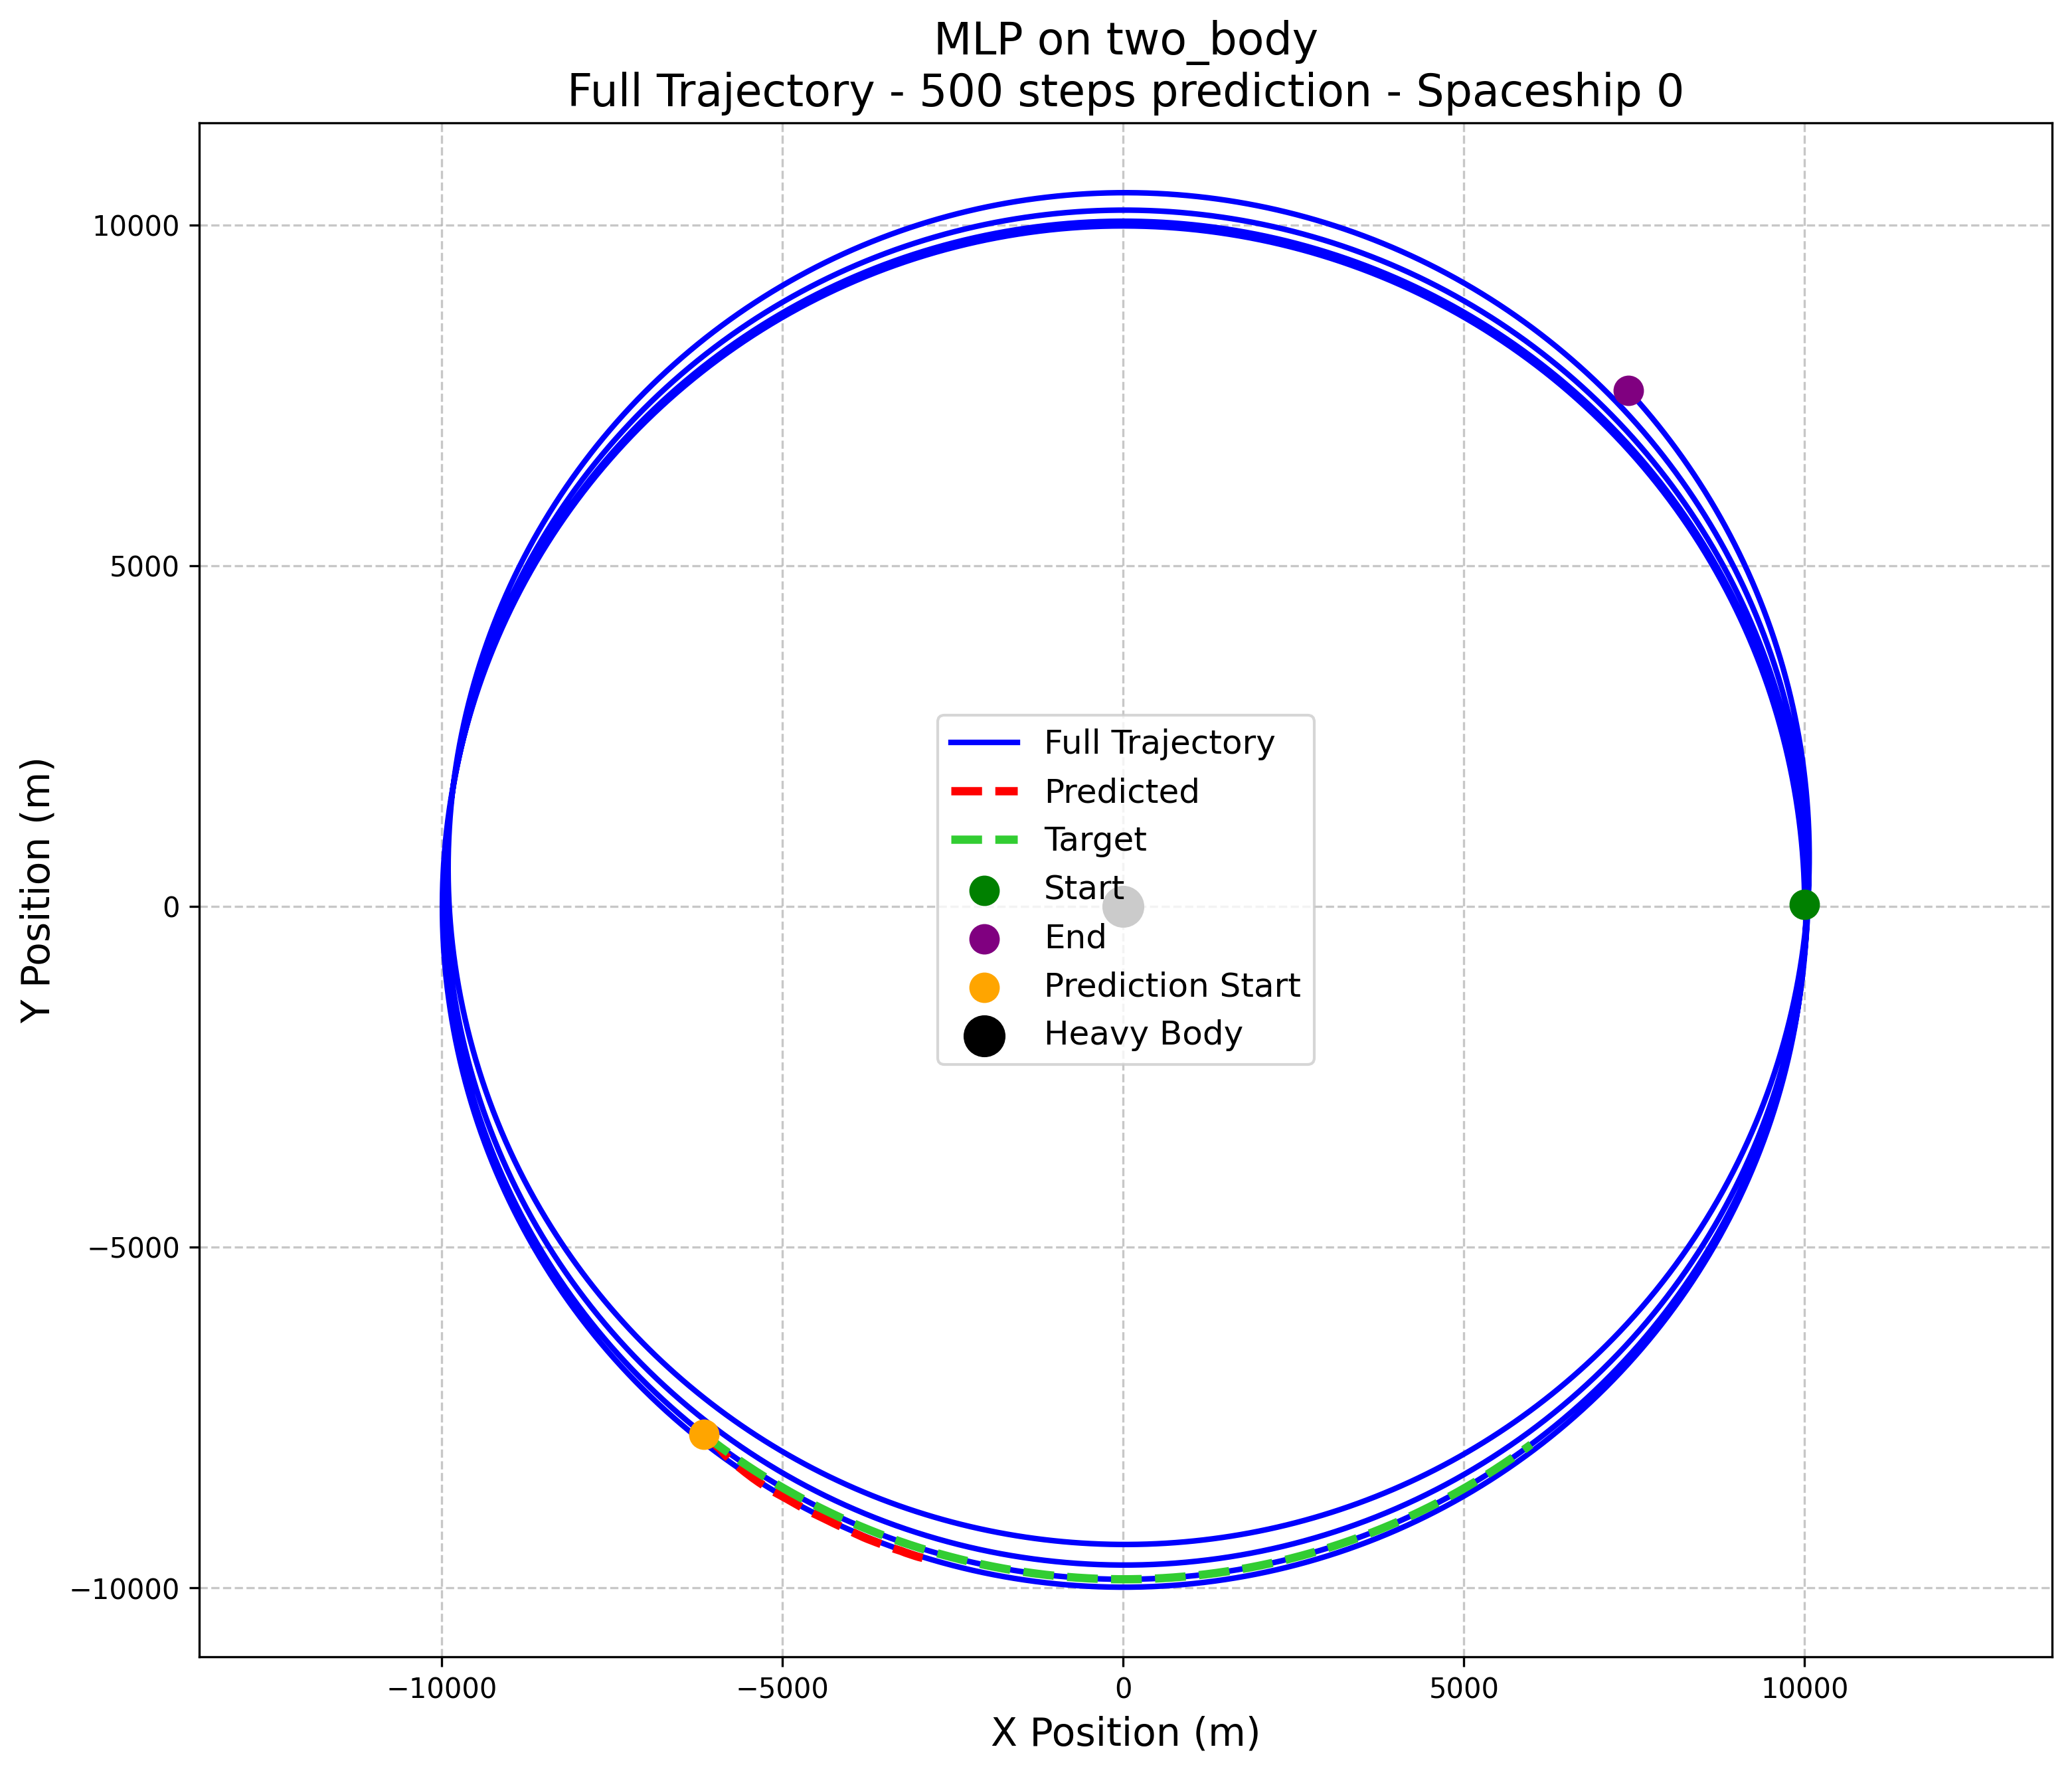
\includegraphics[width=0.27\textwidth]{../inference_results/train/MLP/two_body/500/full_trajectory_spaceship_0.png} &
      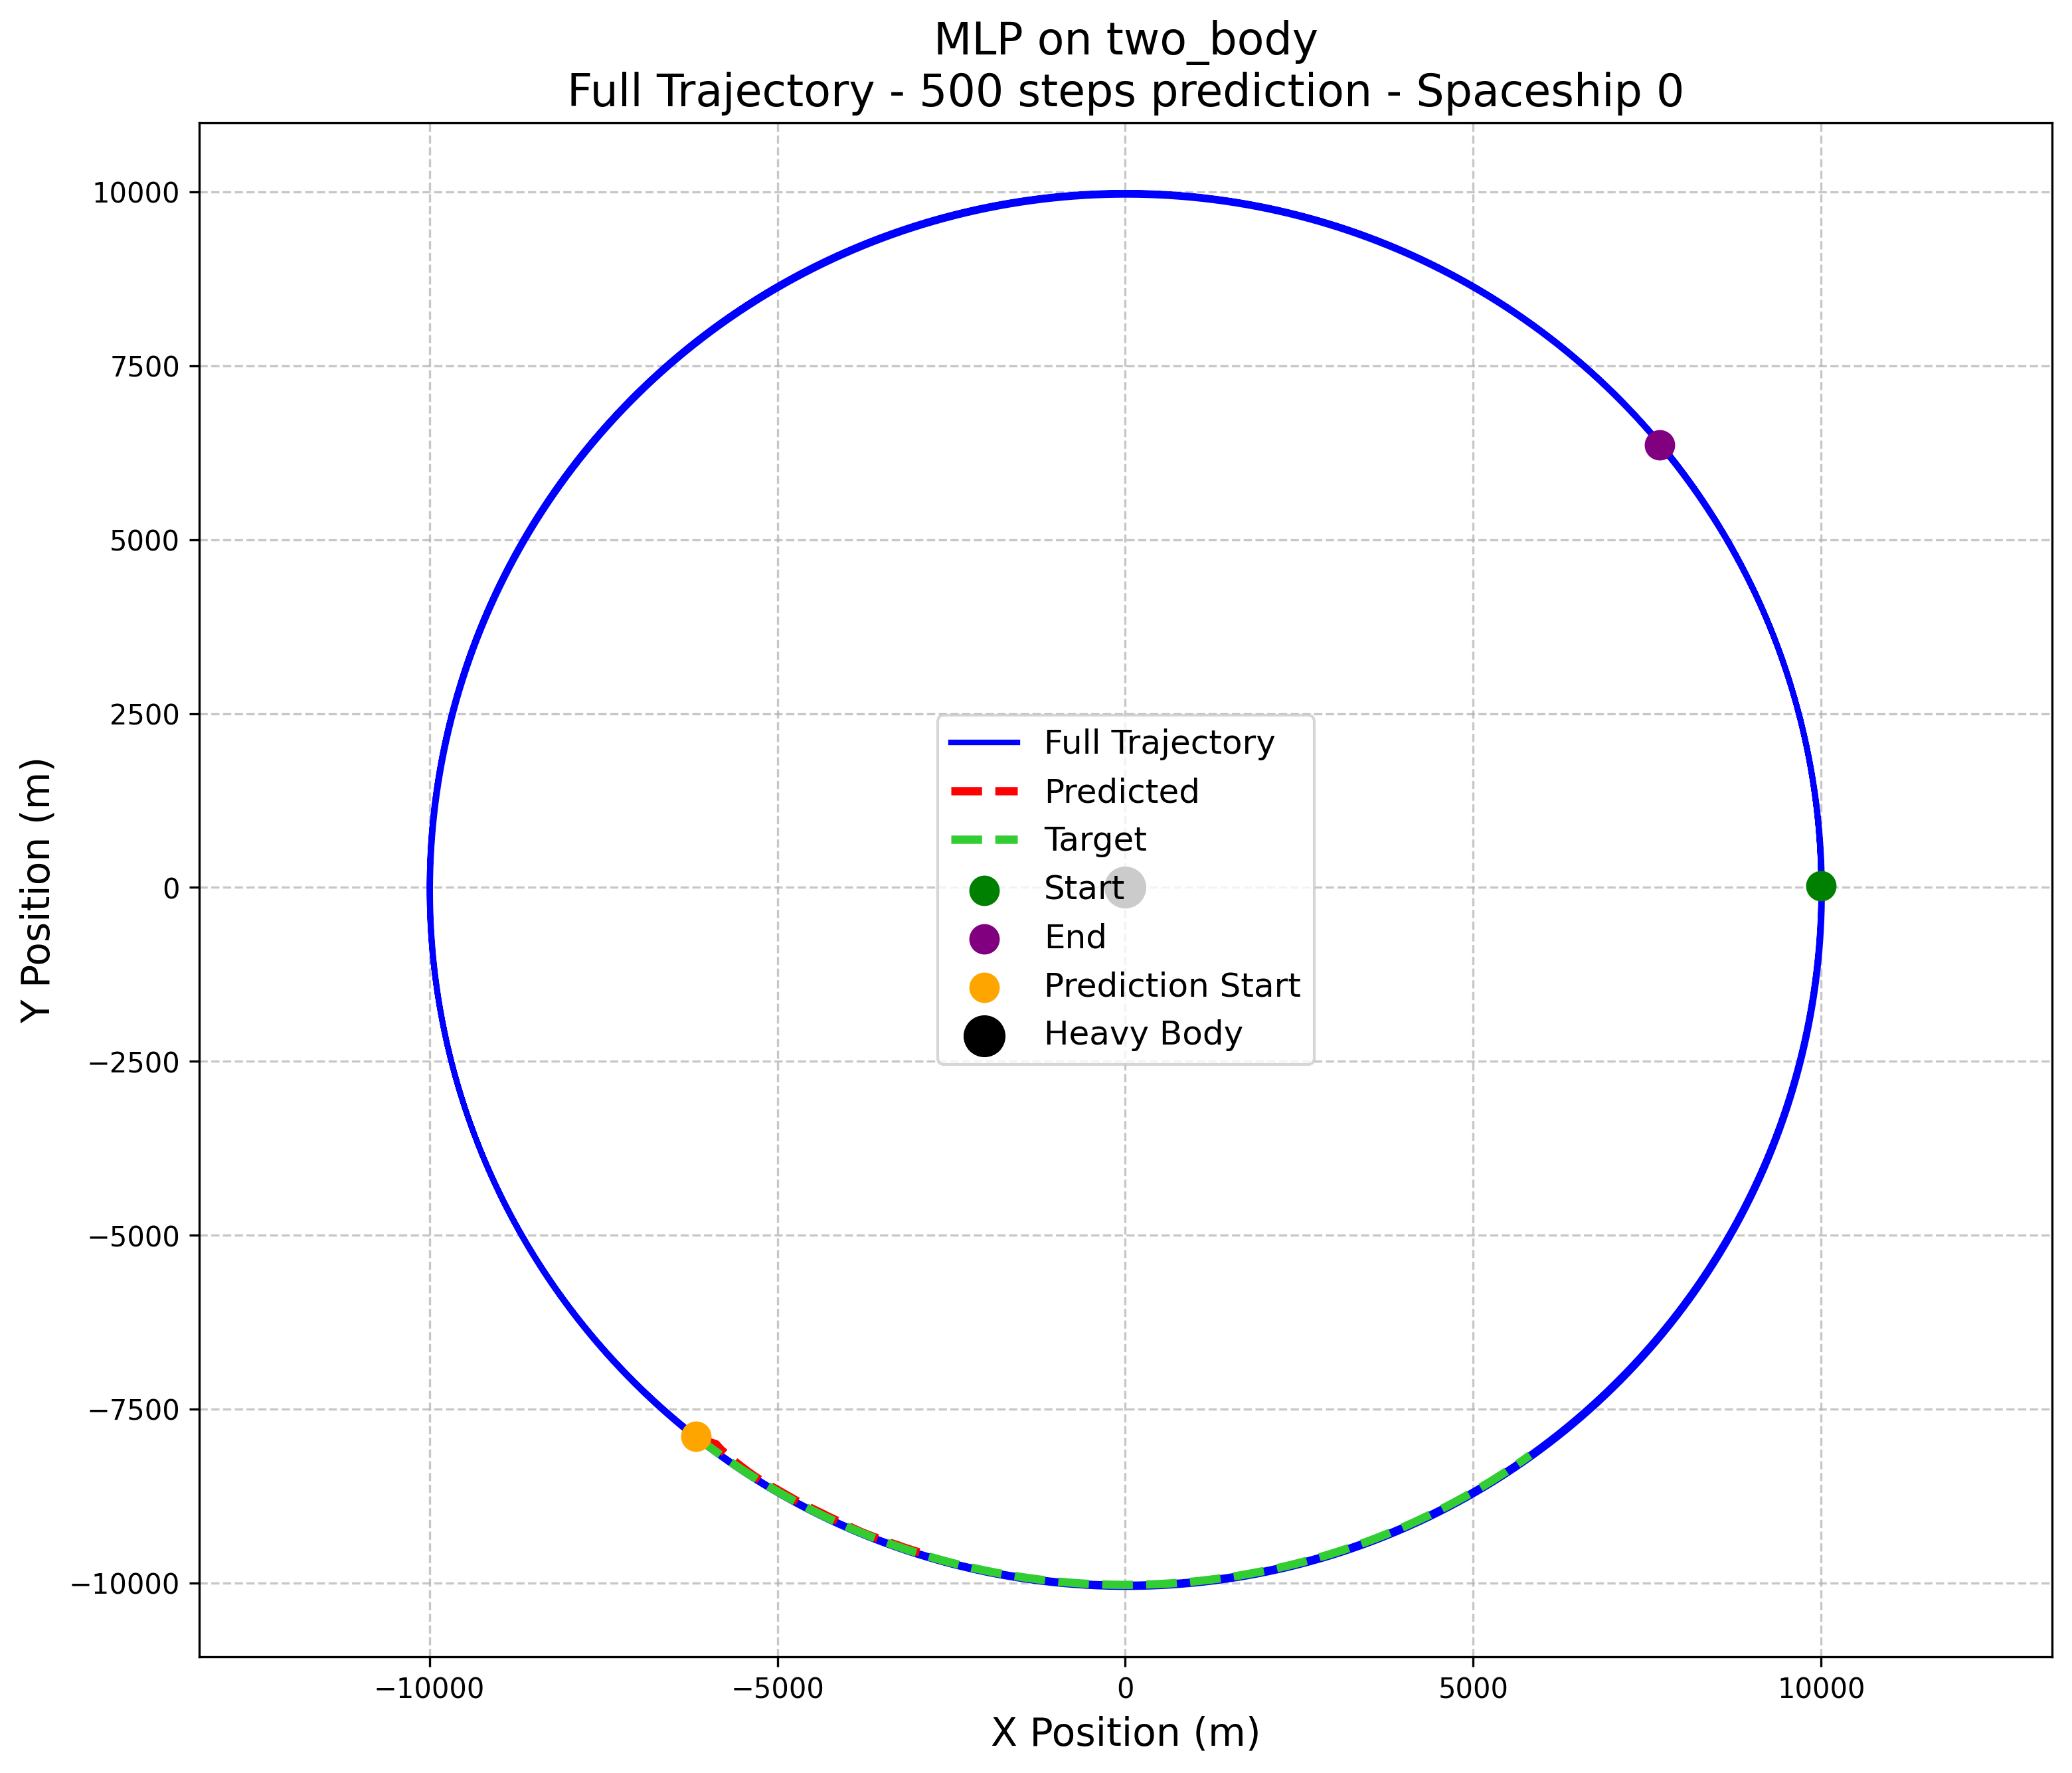
\includegraphics[width=0.27\textwidth]{../inference_results/val/MLP/two_body/500/full_trajectory_spaceship_0.png} &
      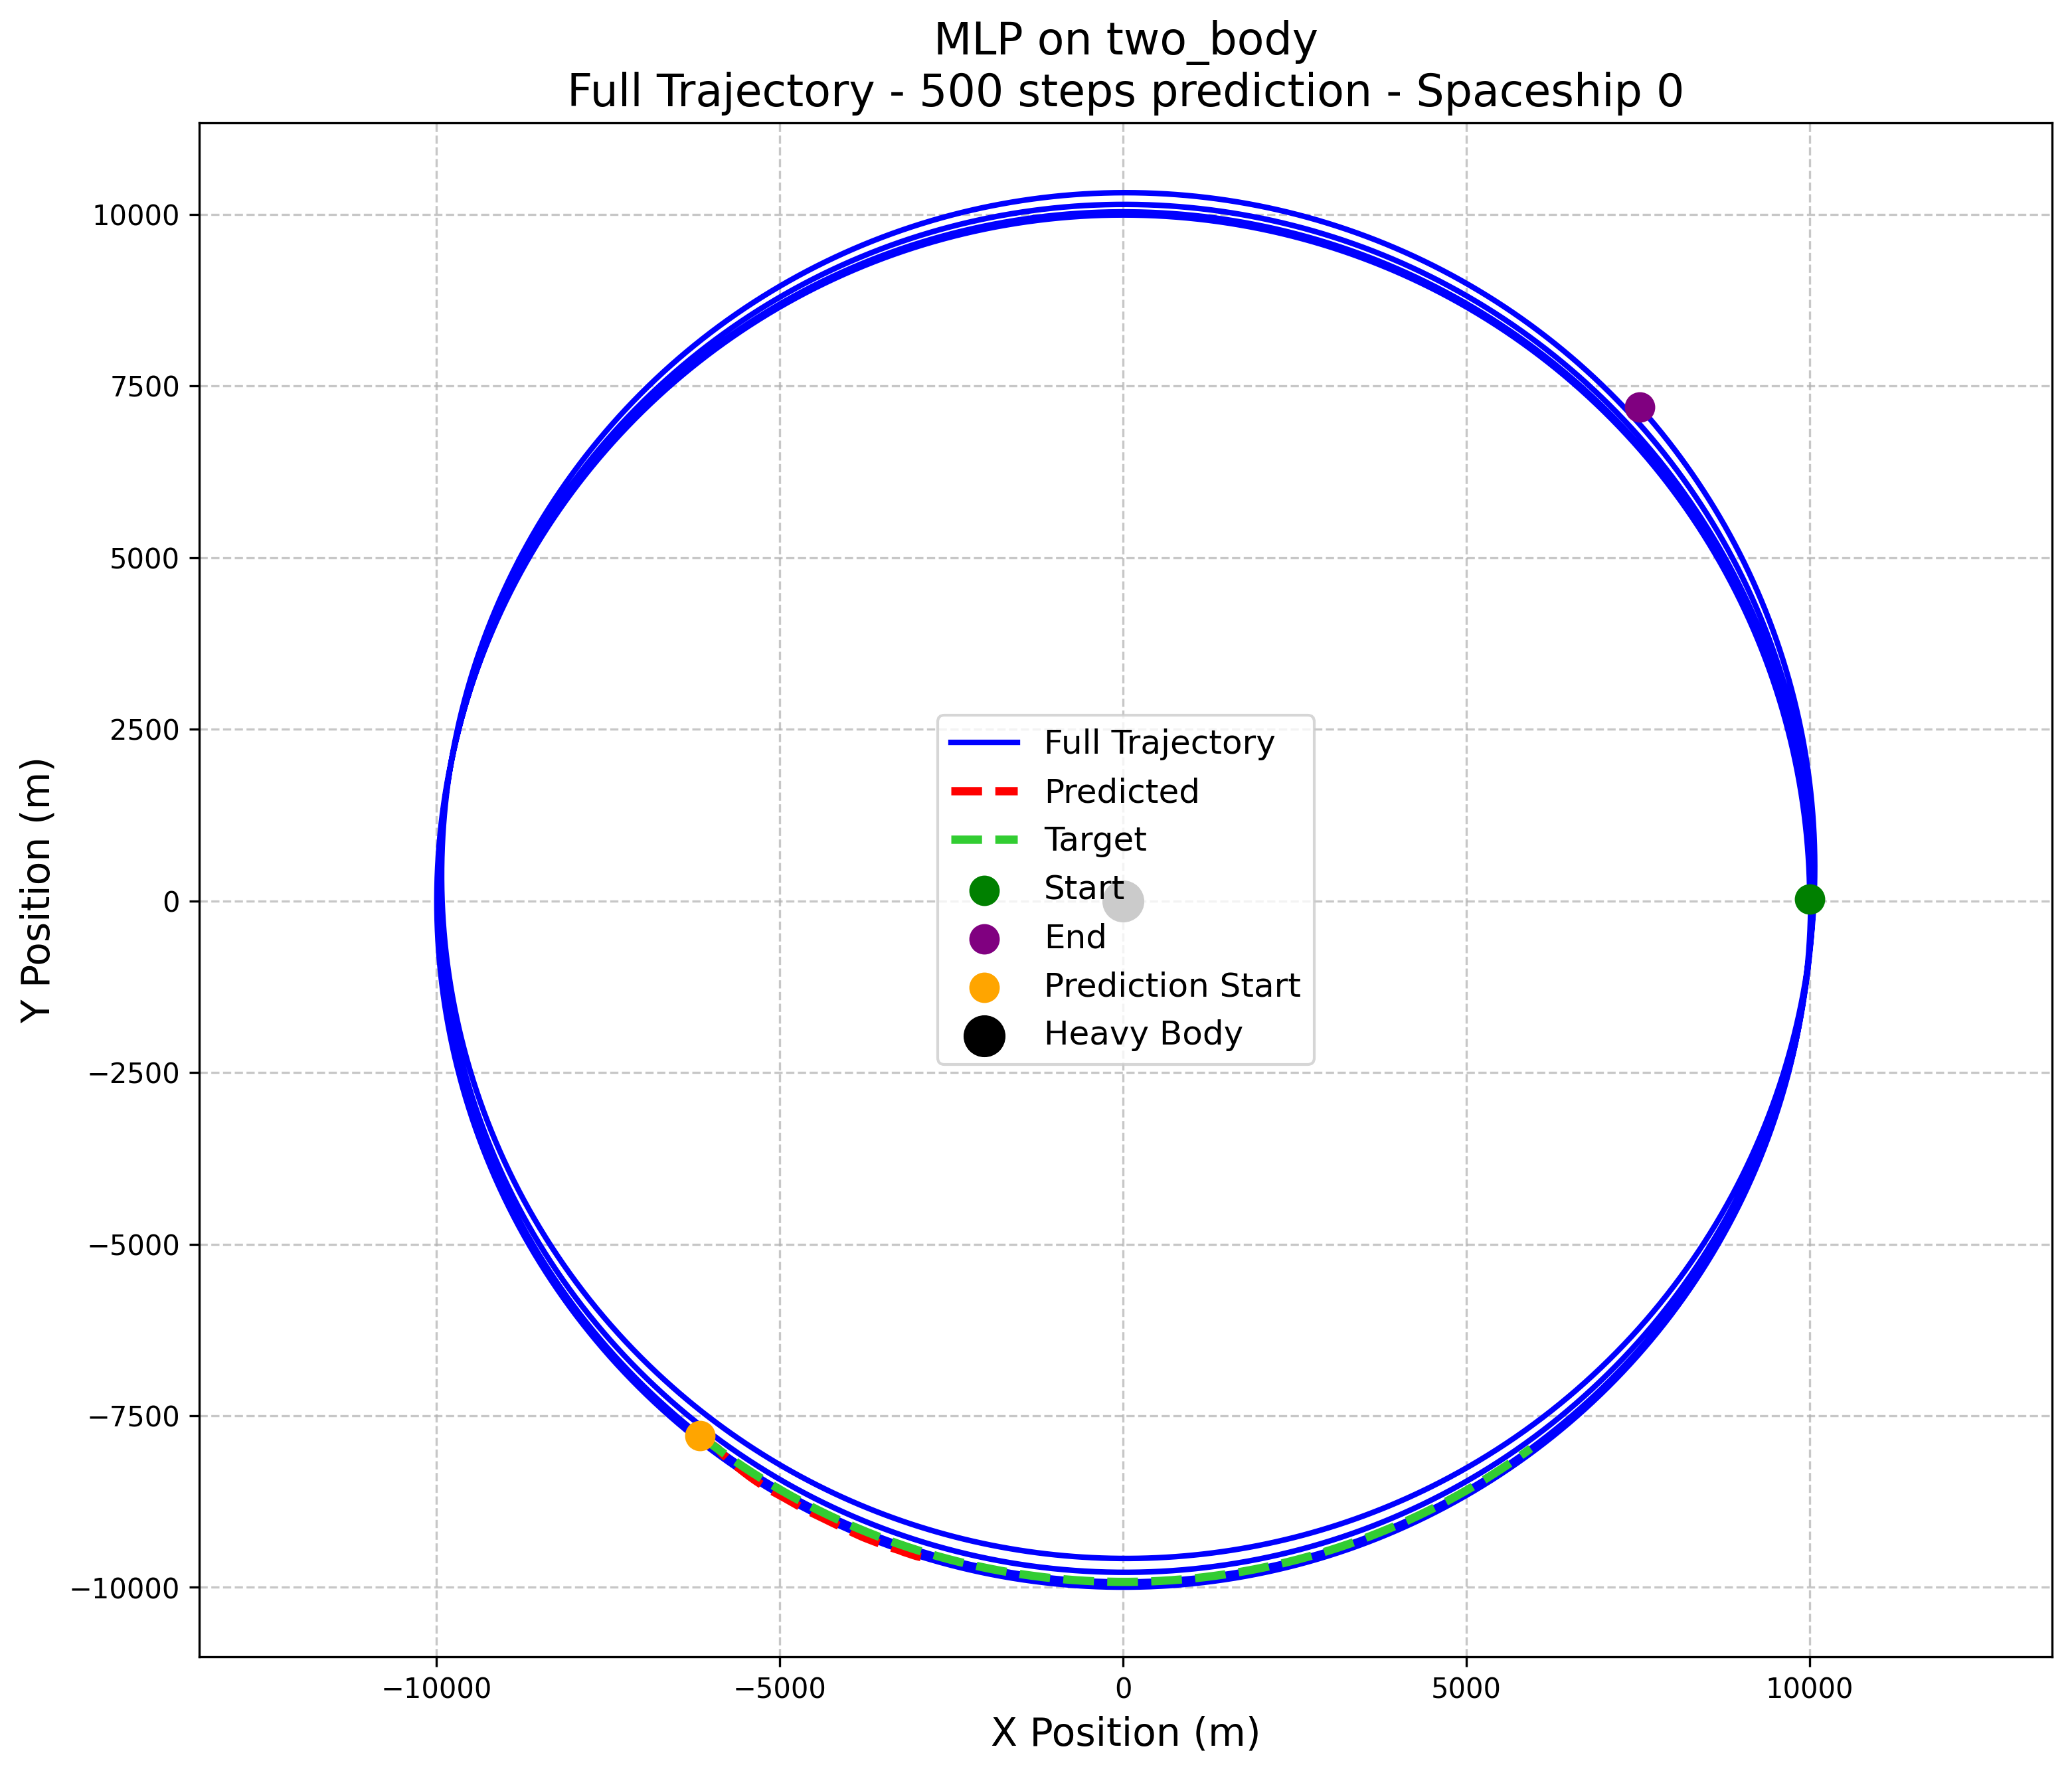
\includegraphics[width=0.27\textwidth]{../inference_results/test/MLP/two_body/500/full_trajectory_spaceship_0.png} \\
      LSTM &
      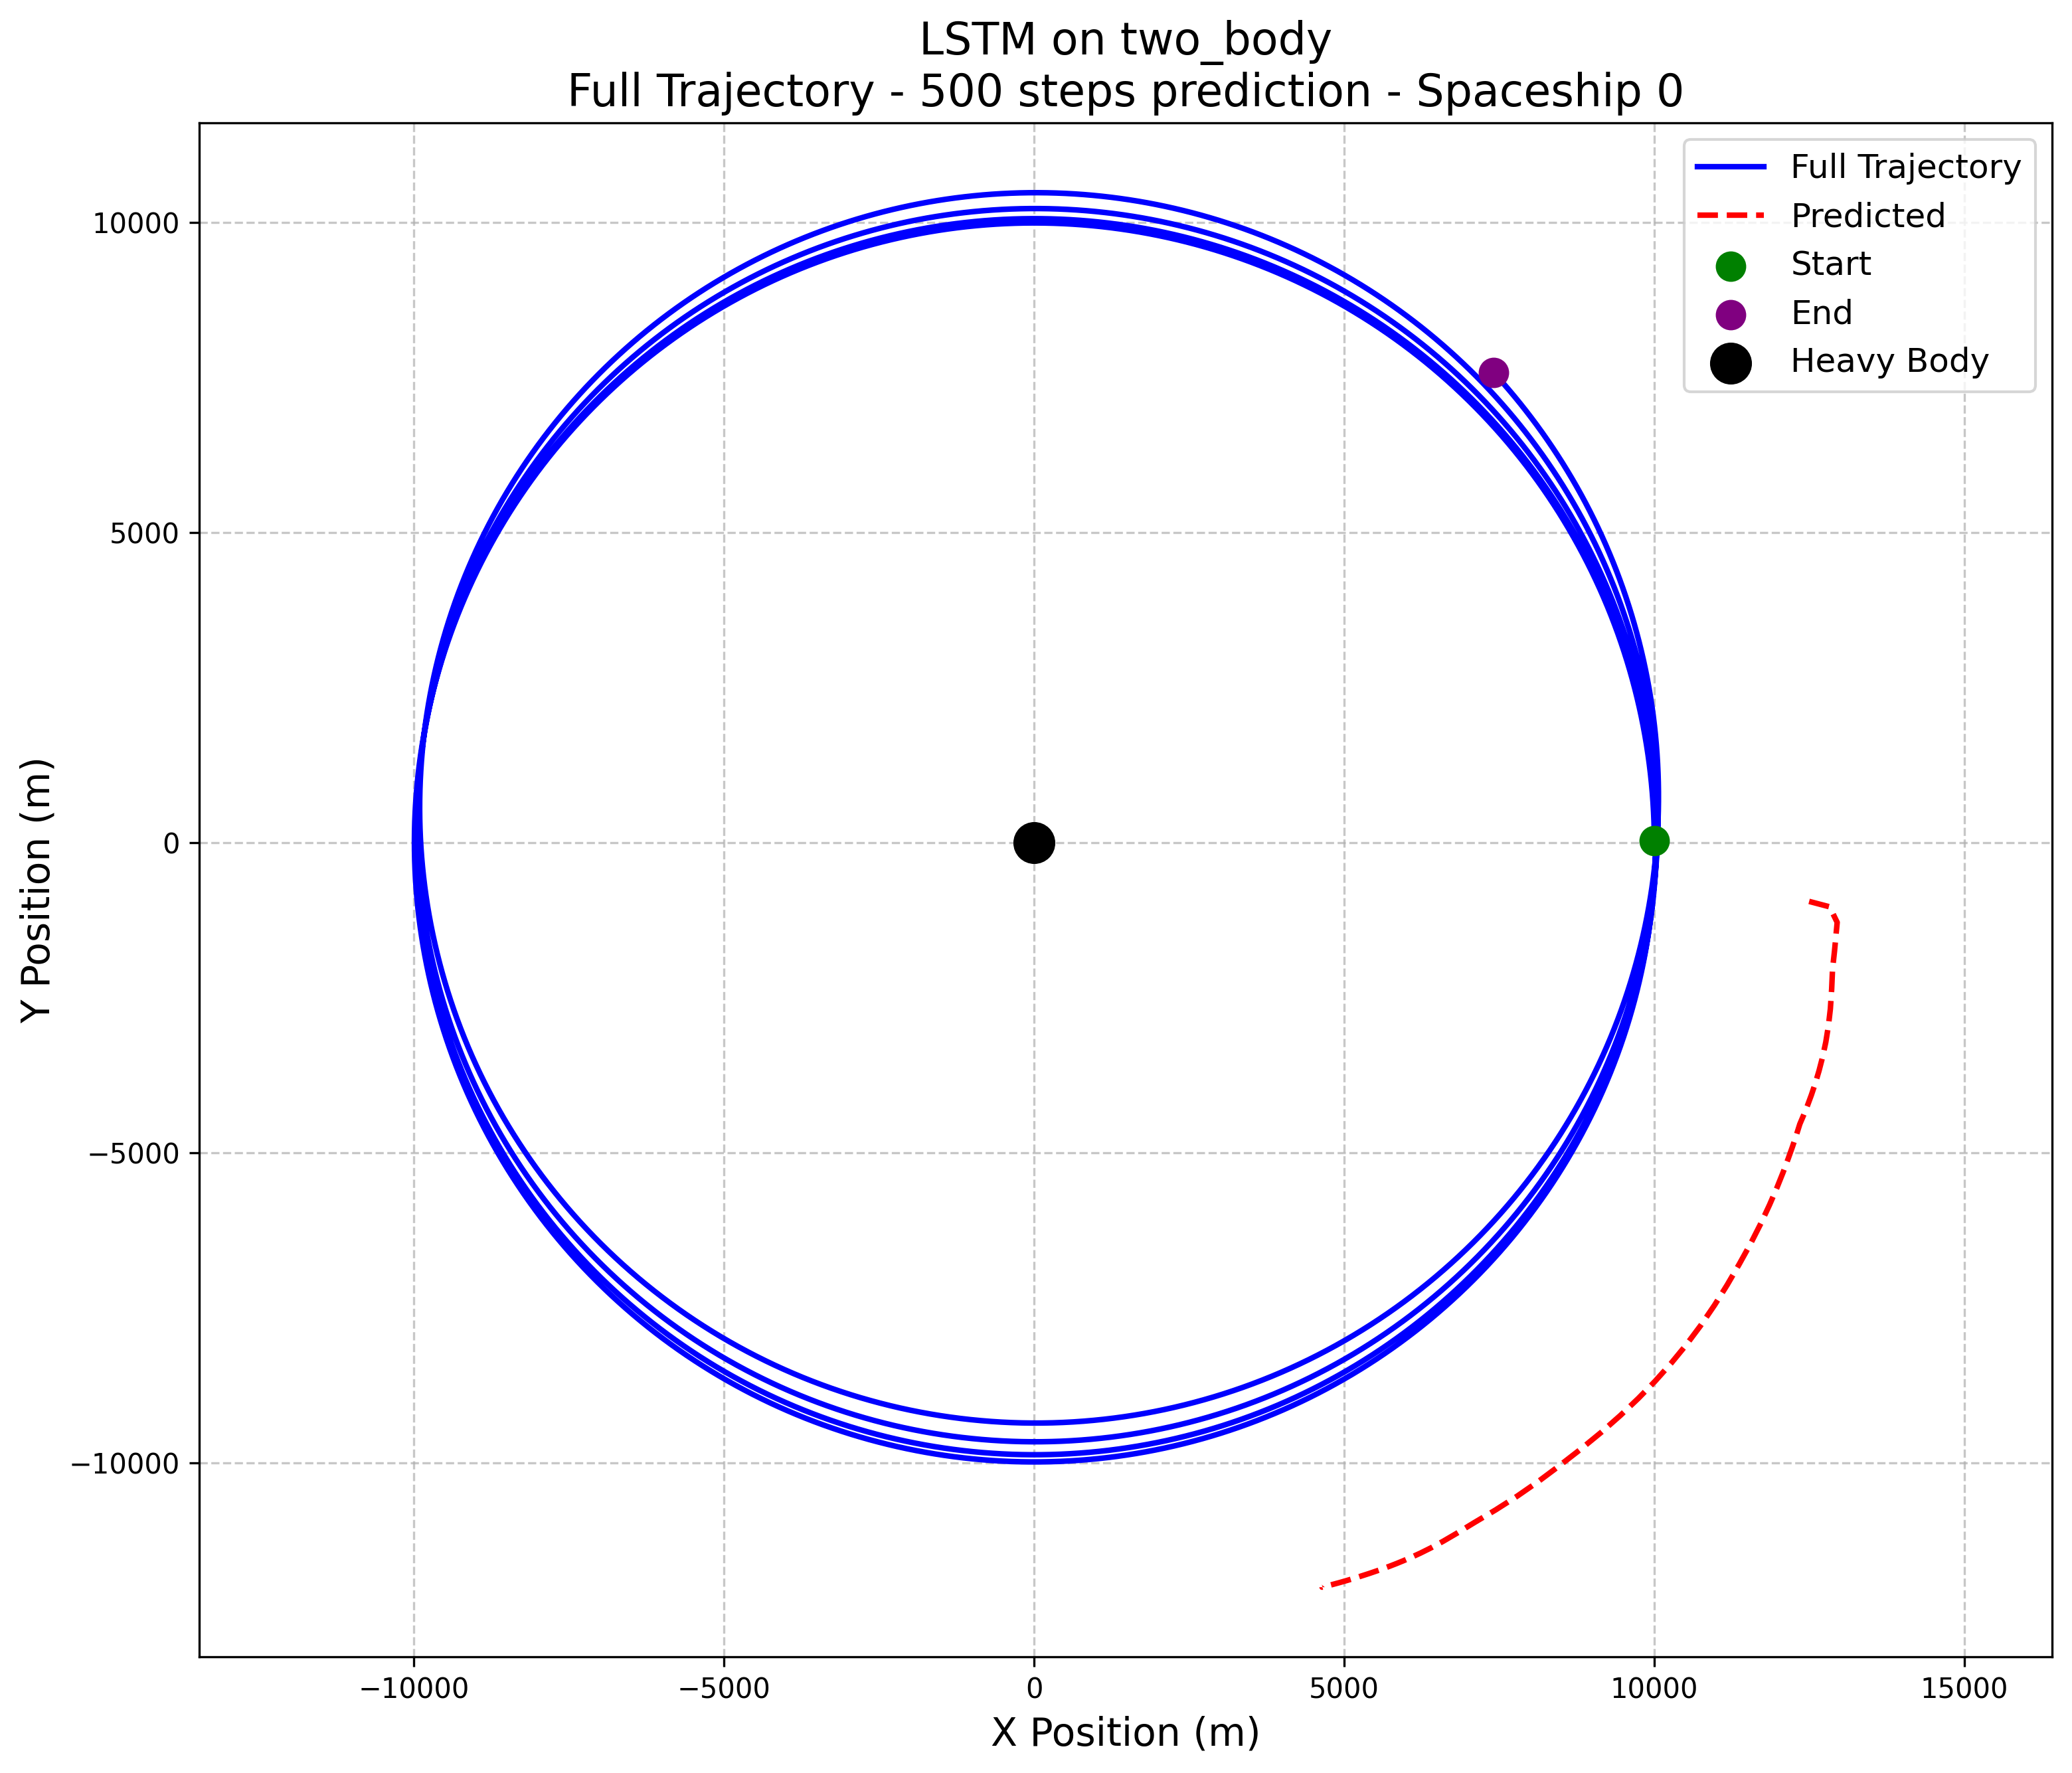
\includegraphics[width=0.27\textwidth]{../inference_results/train/LSTM/two_body/500/full_trajectory_spaceship_0.png} &
      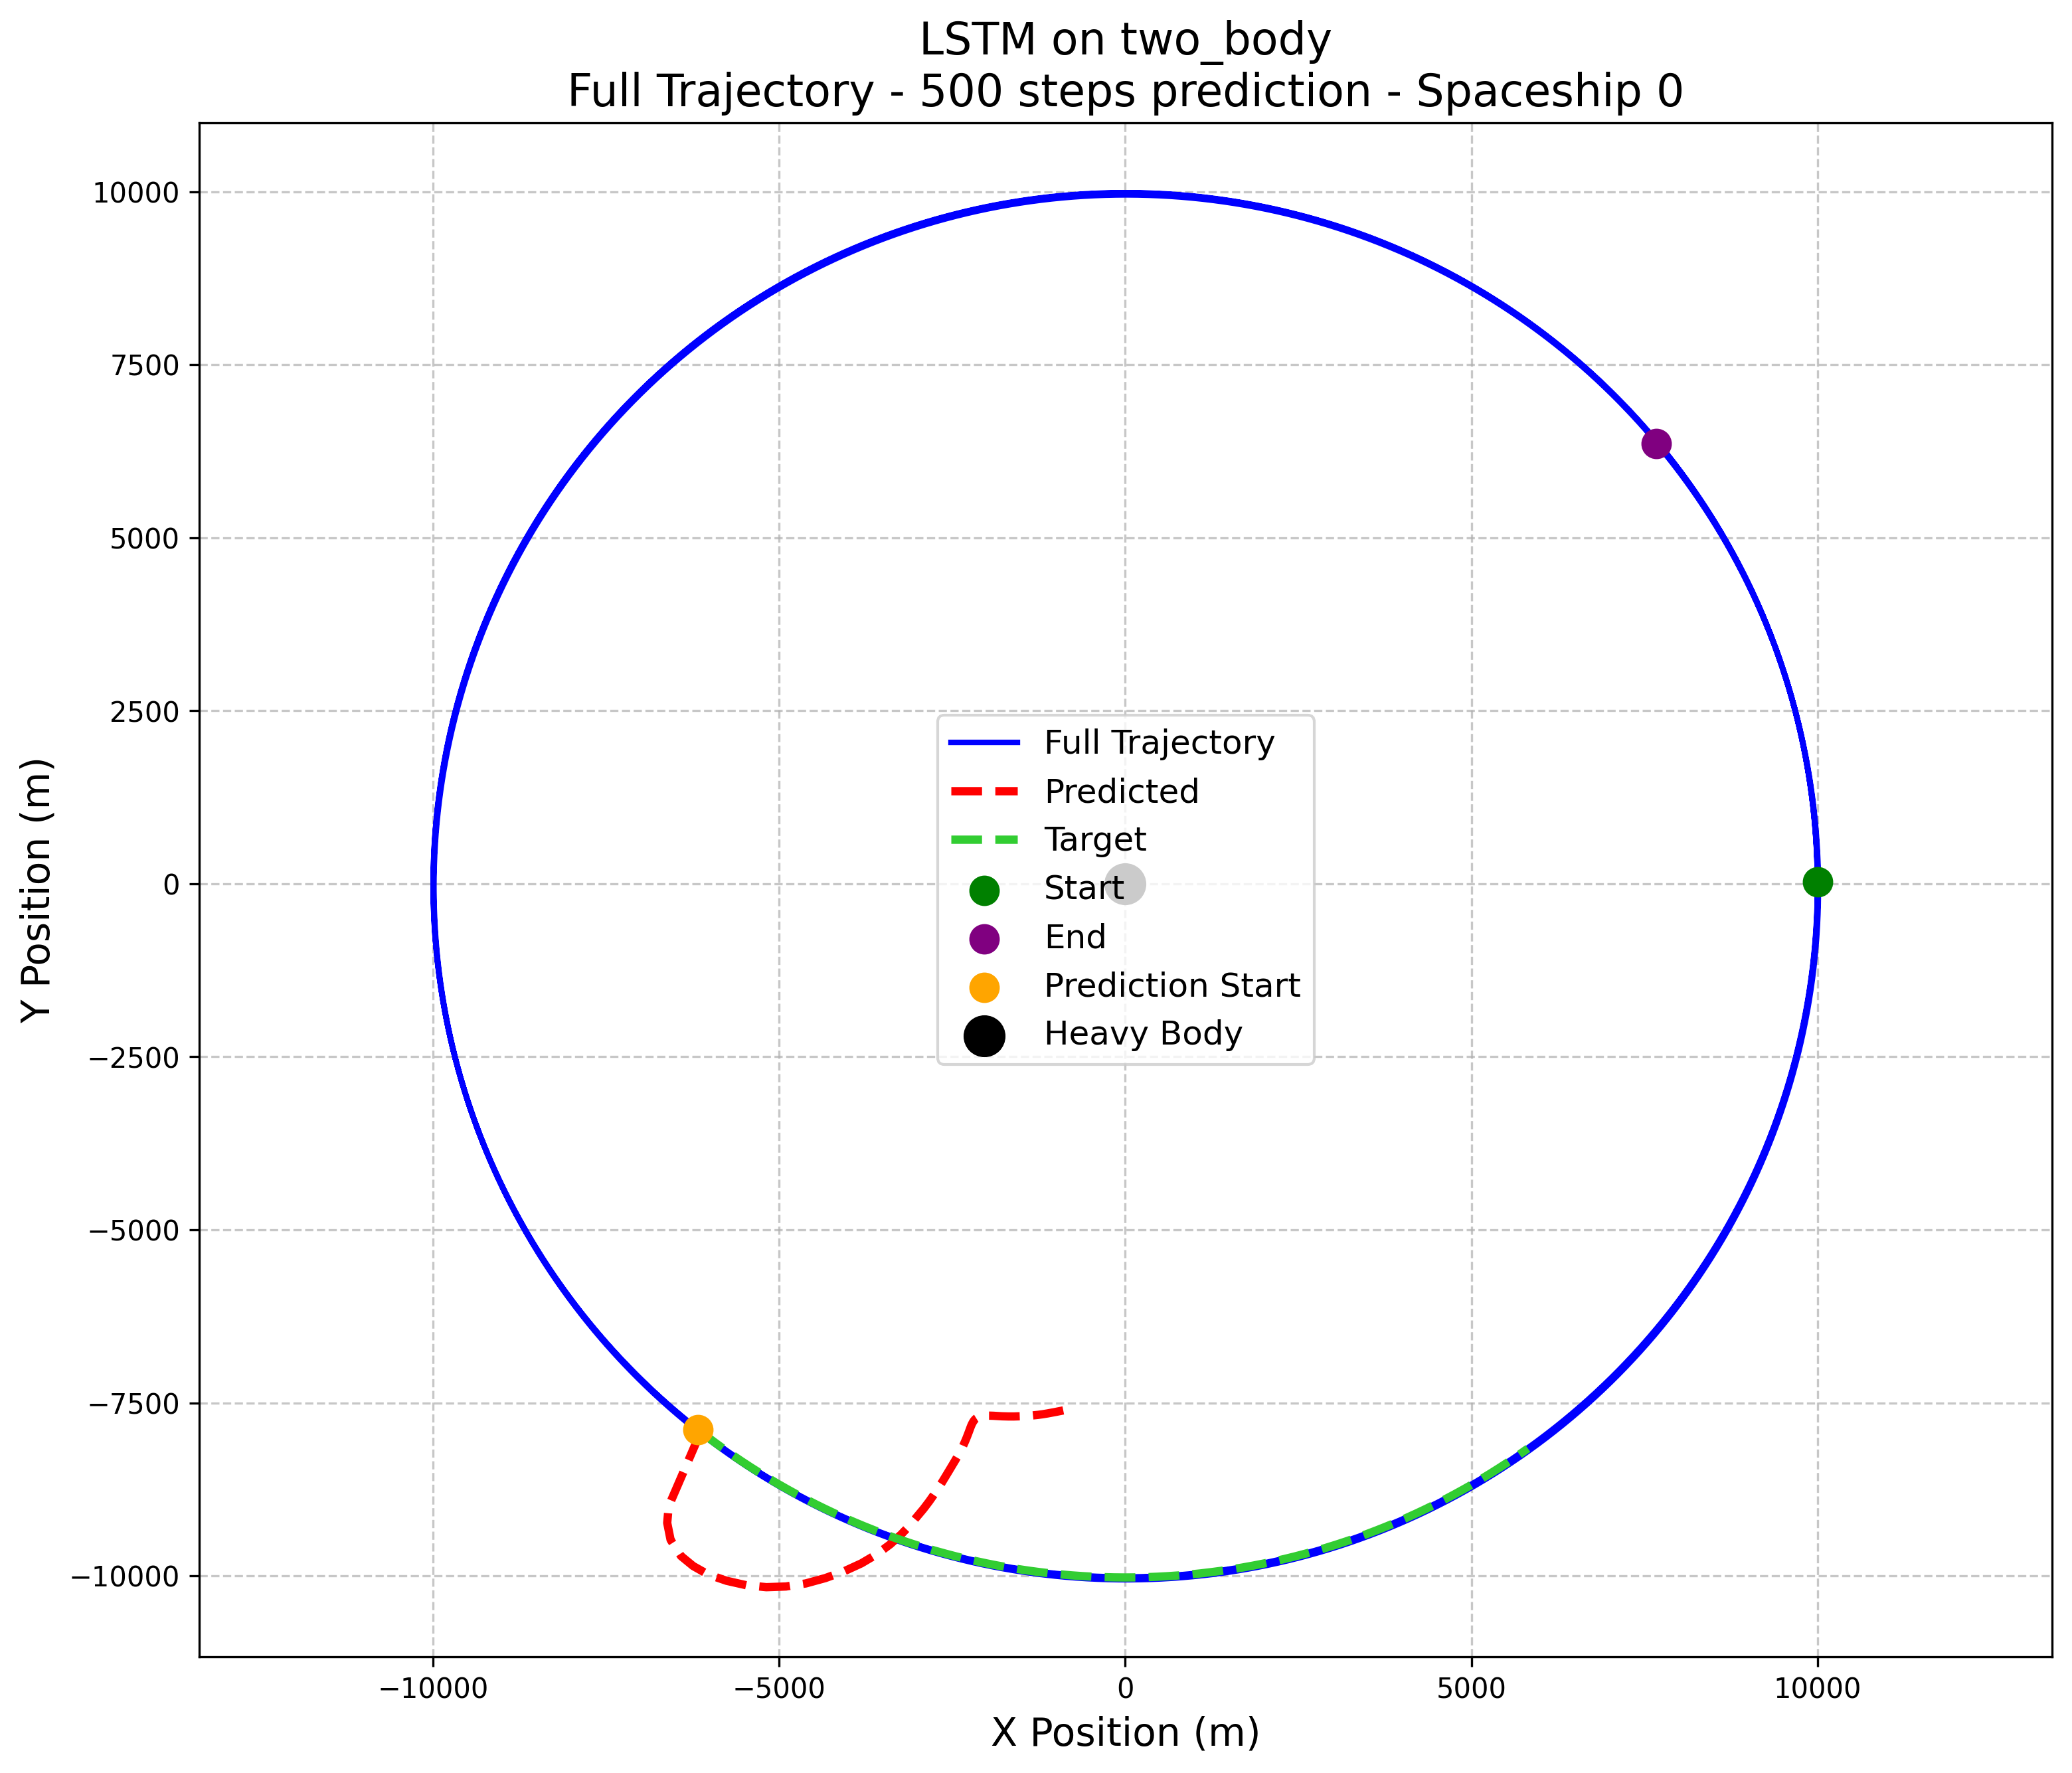
\includegraphics[width=0.27\textwidth]{../inference_results/val/LSTM/two_body/500/full_trajectory_spaceship_0.png} &
      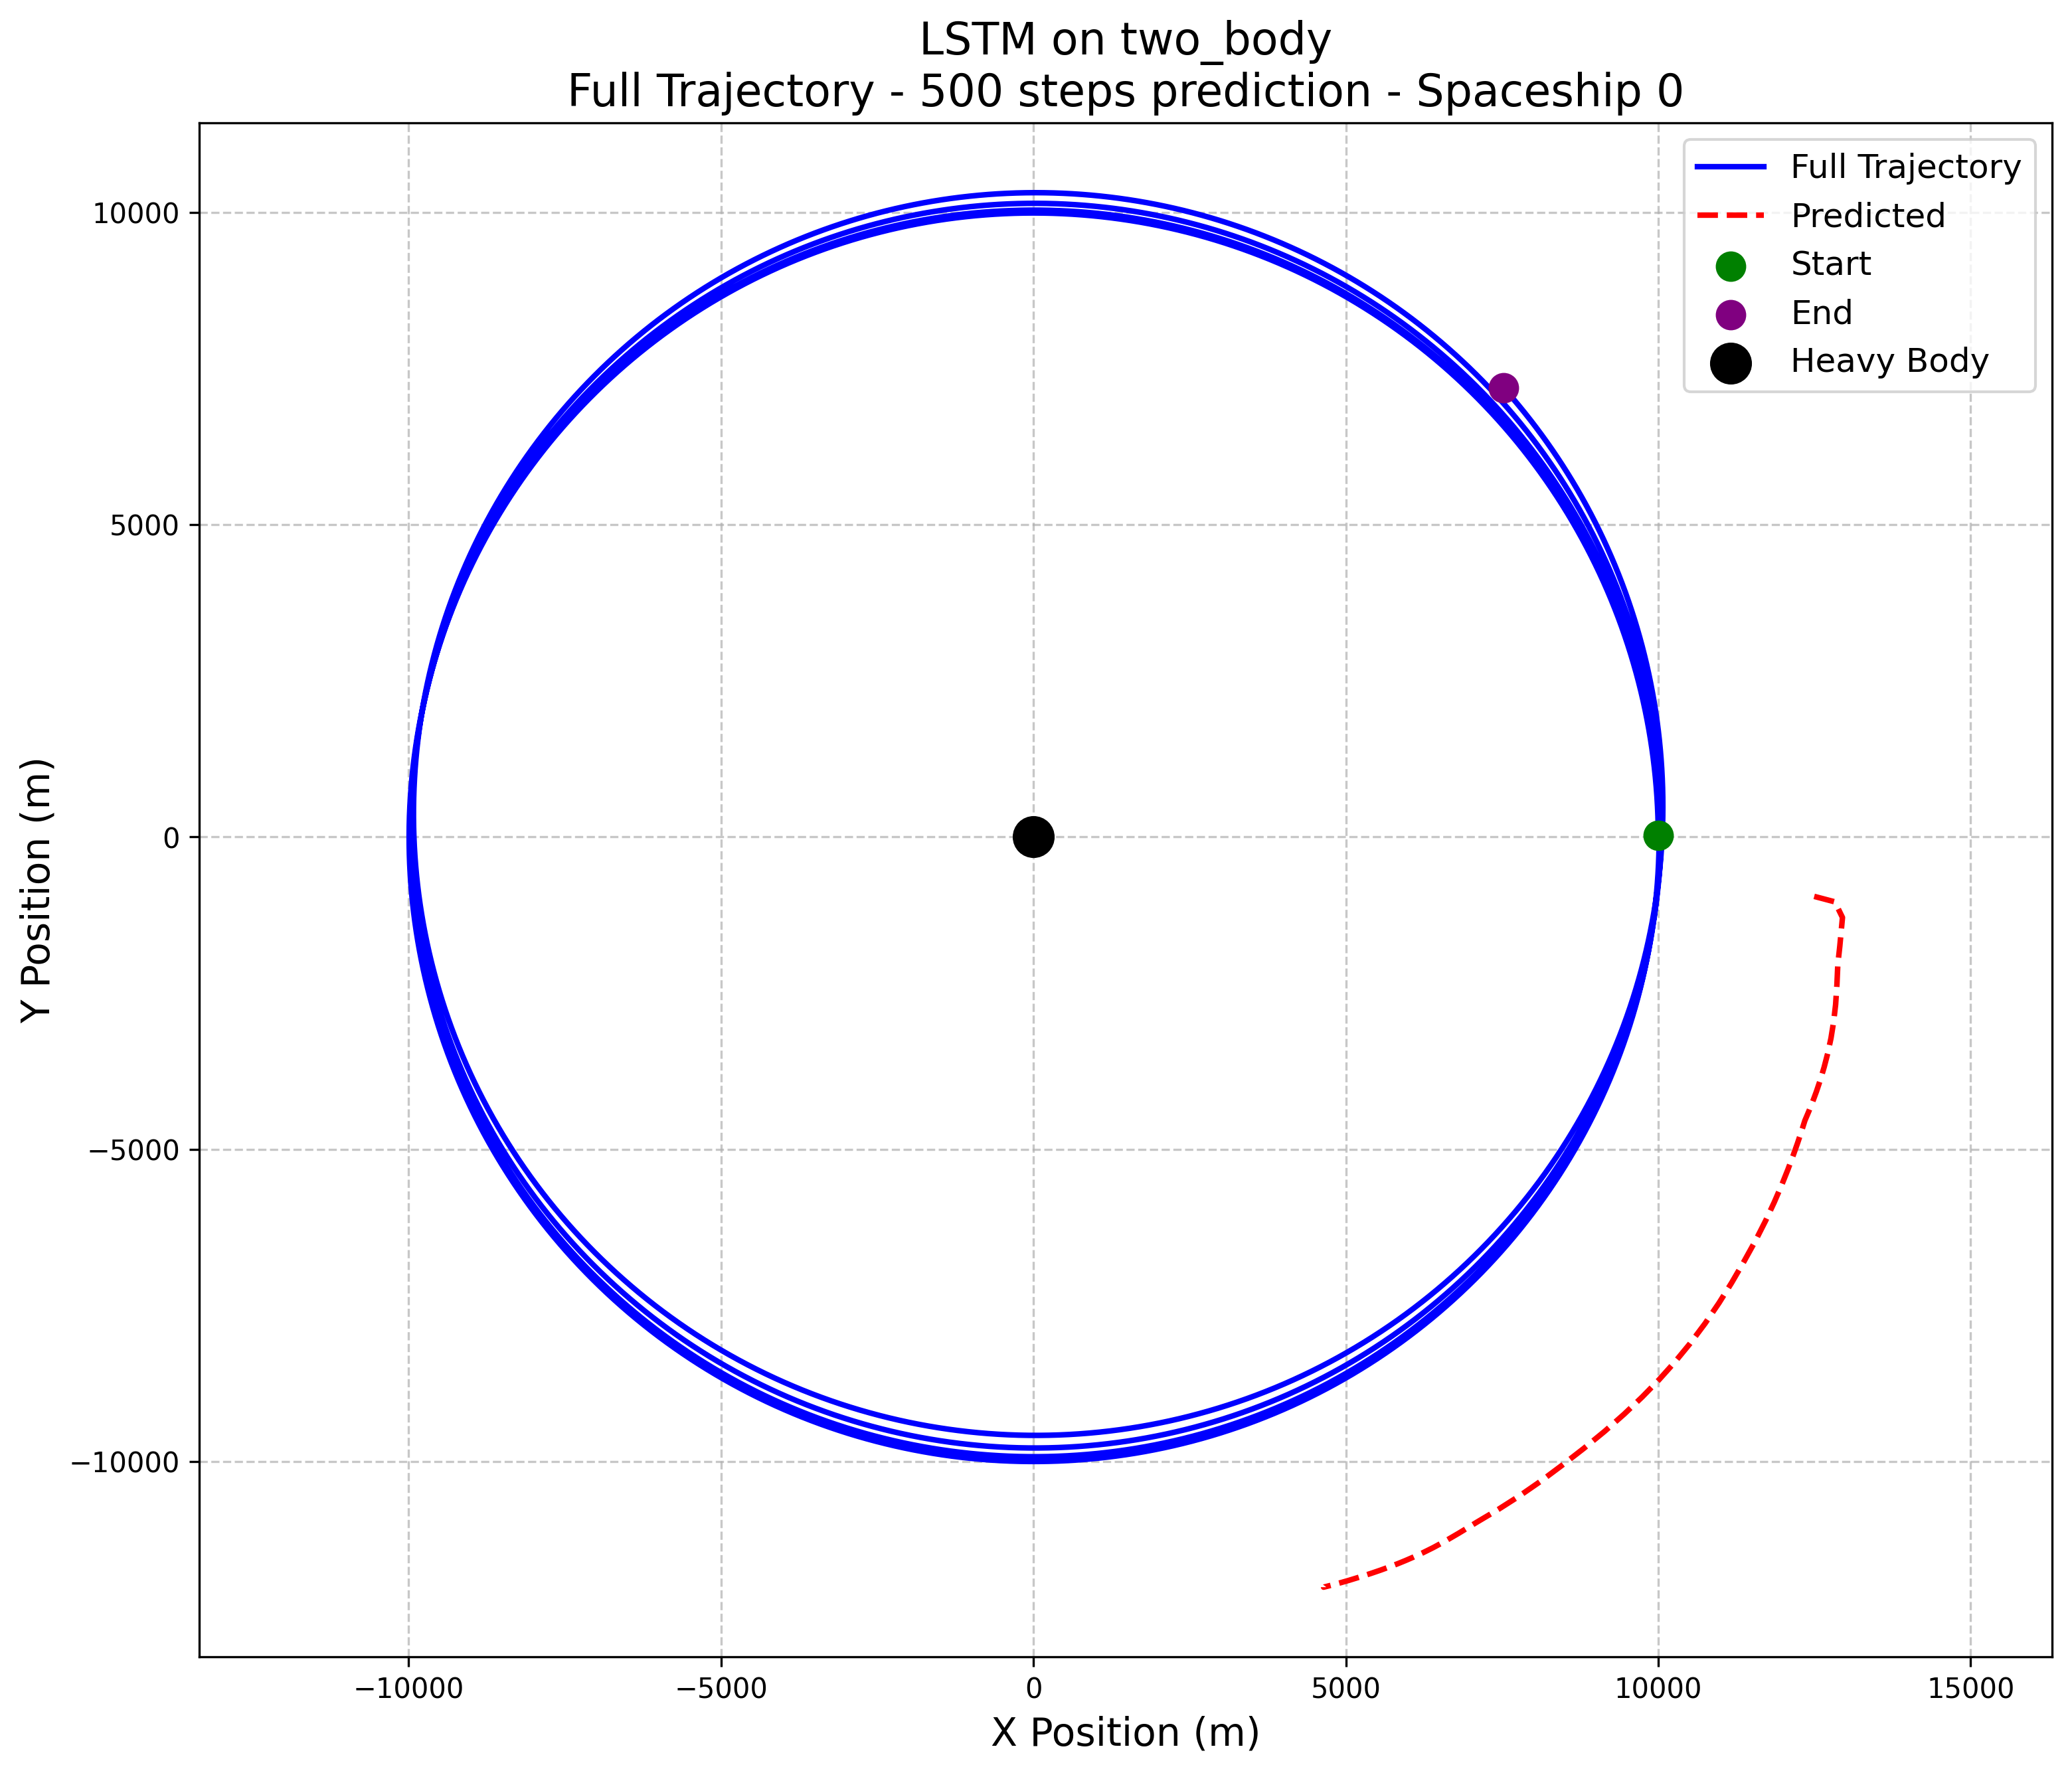
\includegraphics[width=0.27\textwidth]{../inference_results/test/LSTM/two_body/500/full_trajectory_spaceship_0.png} \\
      PINN &
      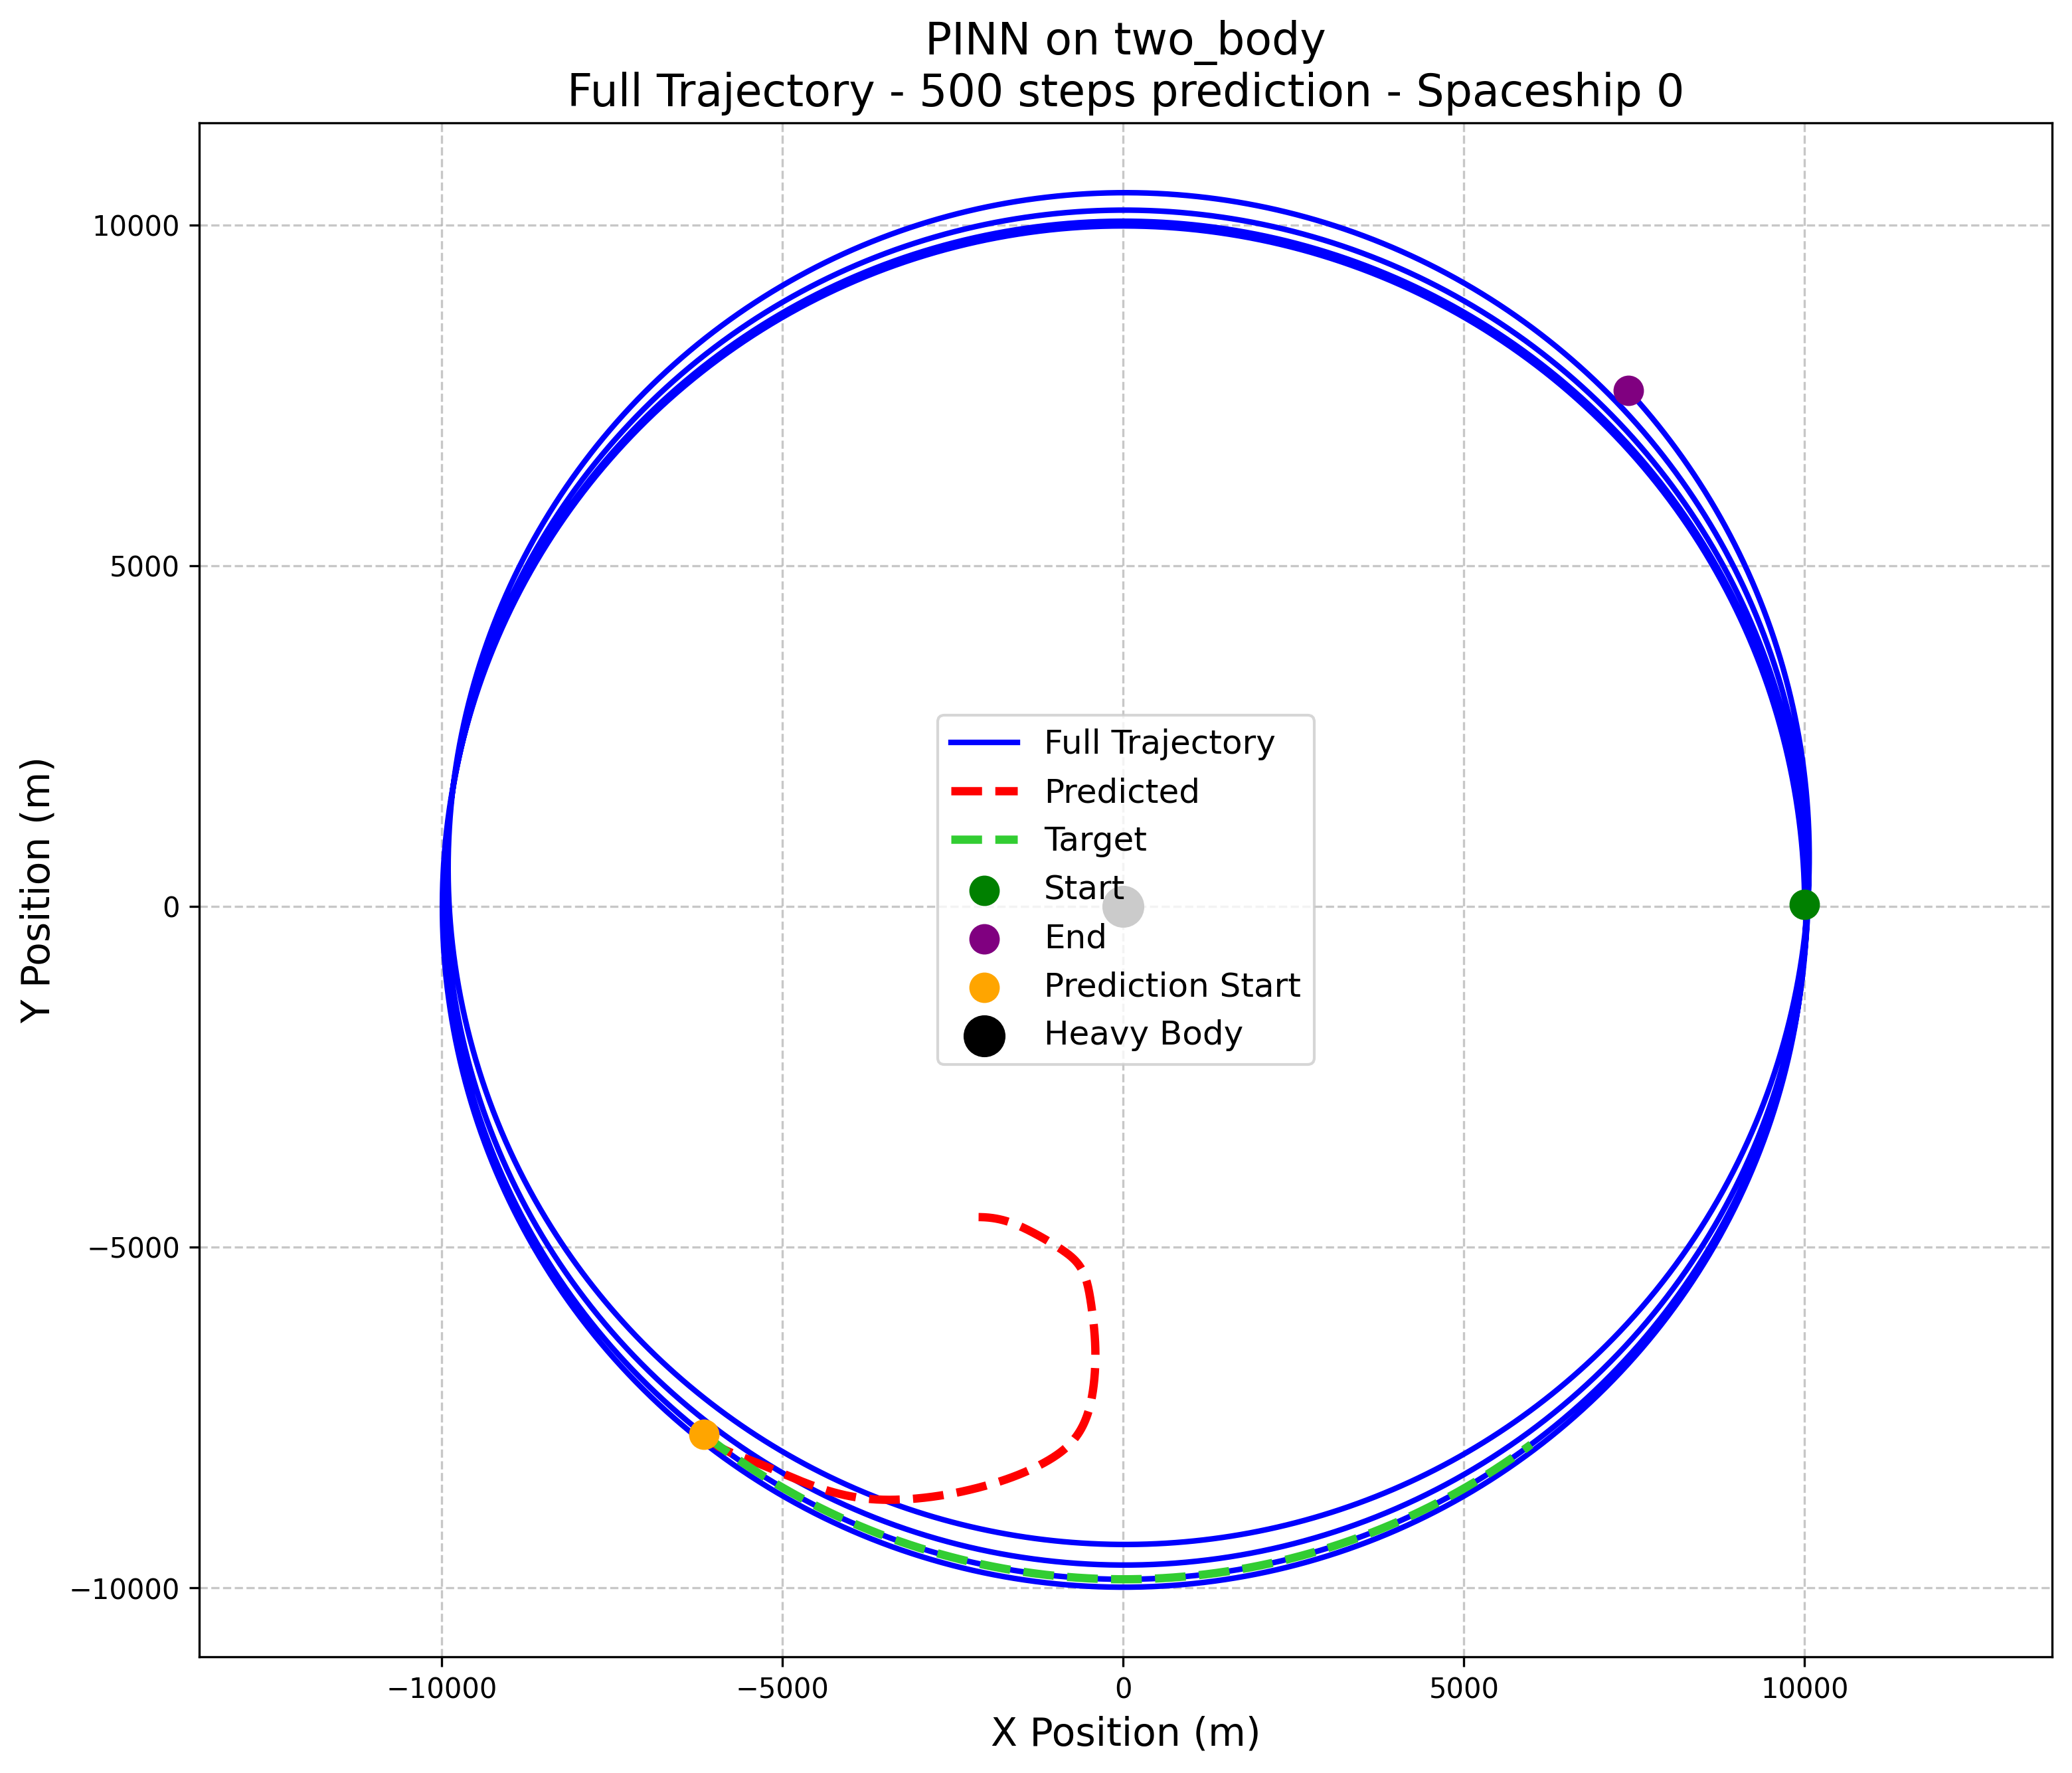
\includegraphics[width=0.27\textwidth]{../inference_results/train/PINN/two_body/500/full_trajectory_spaceship_0.png} &
      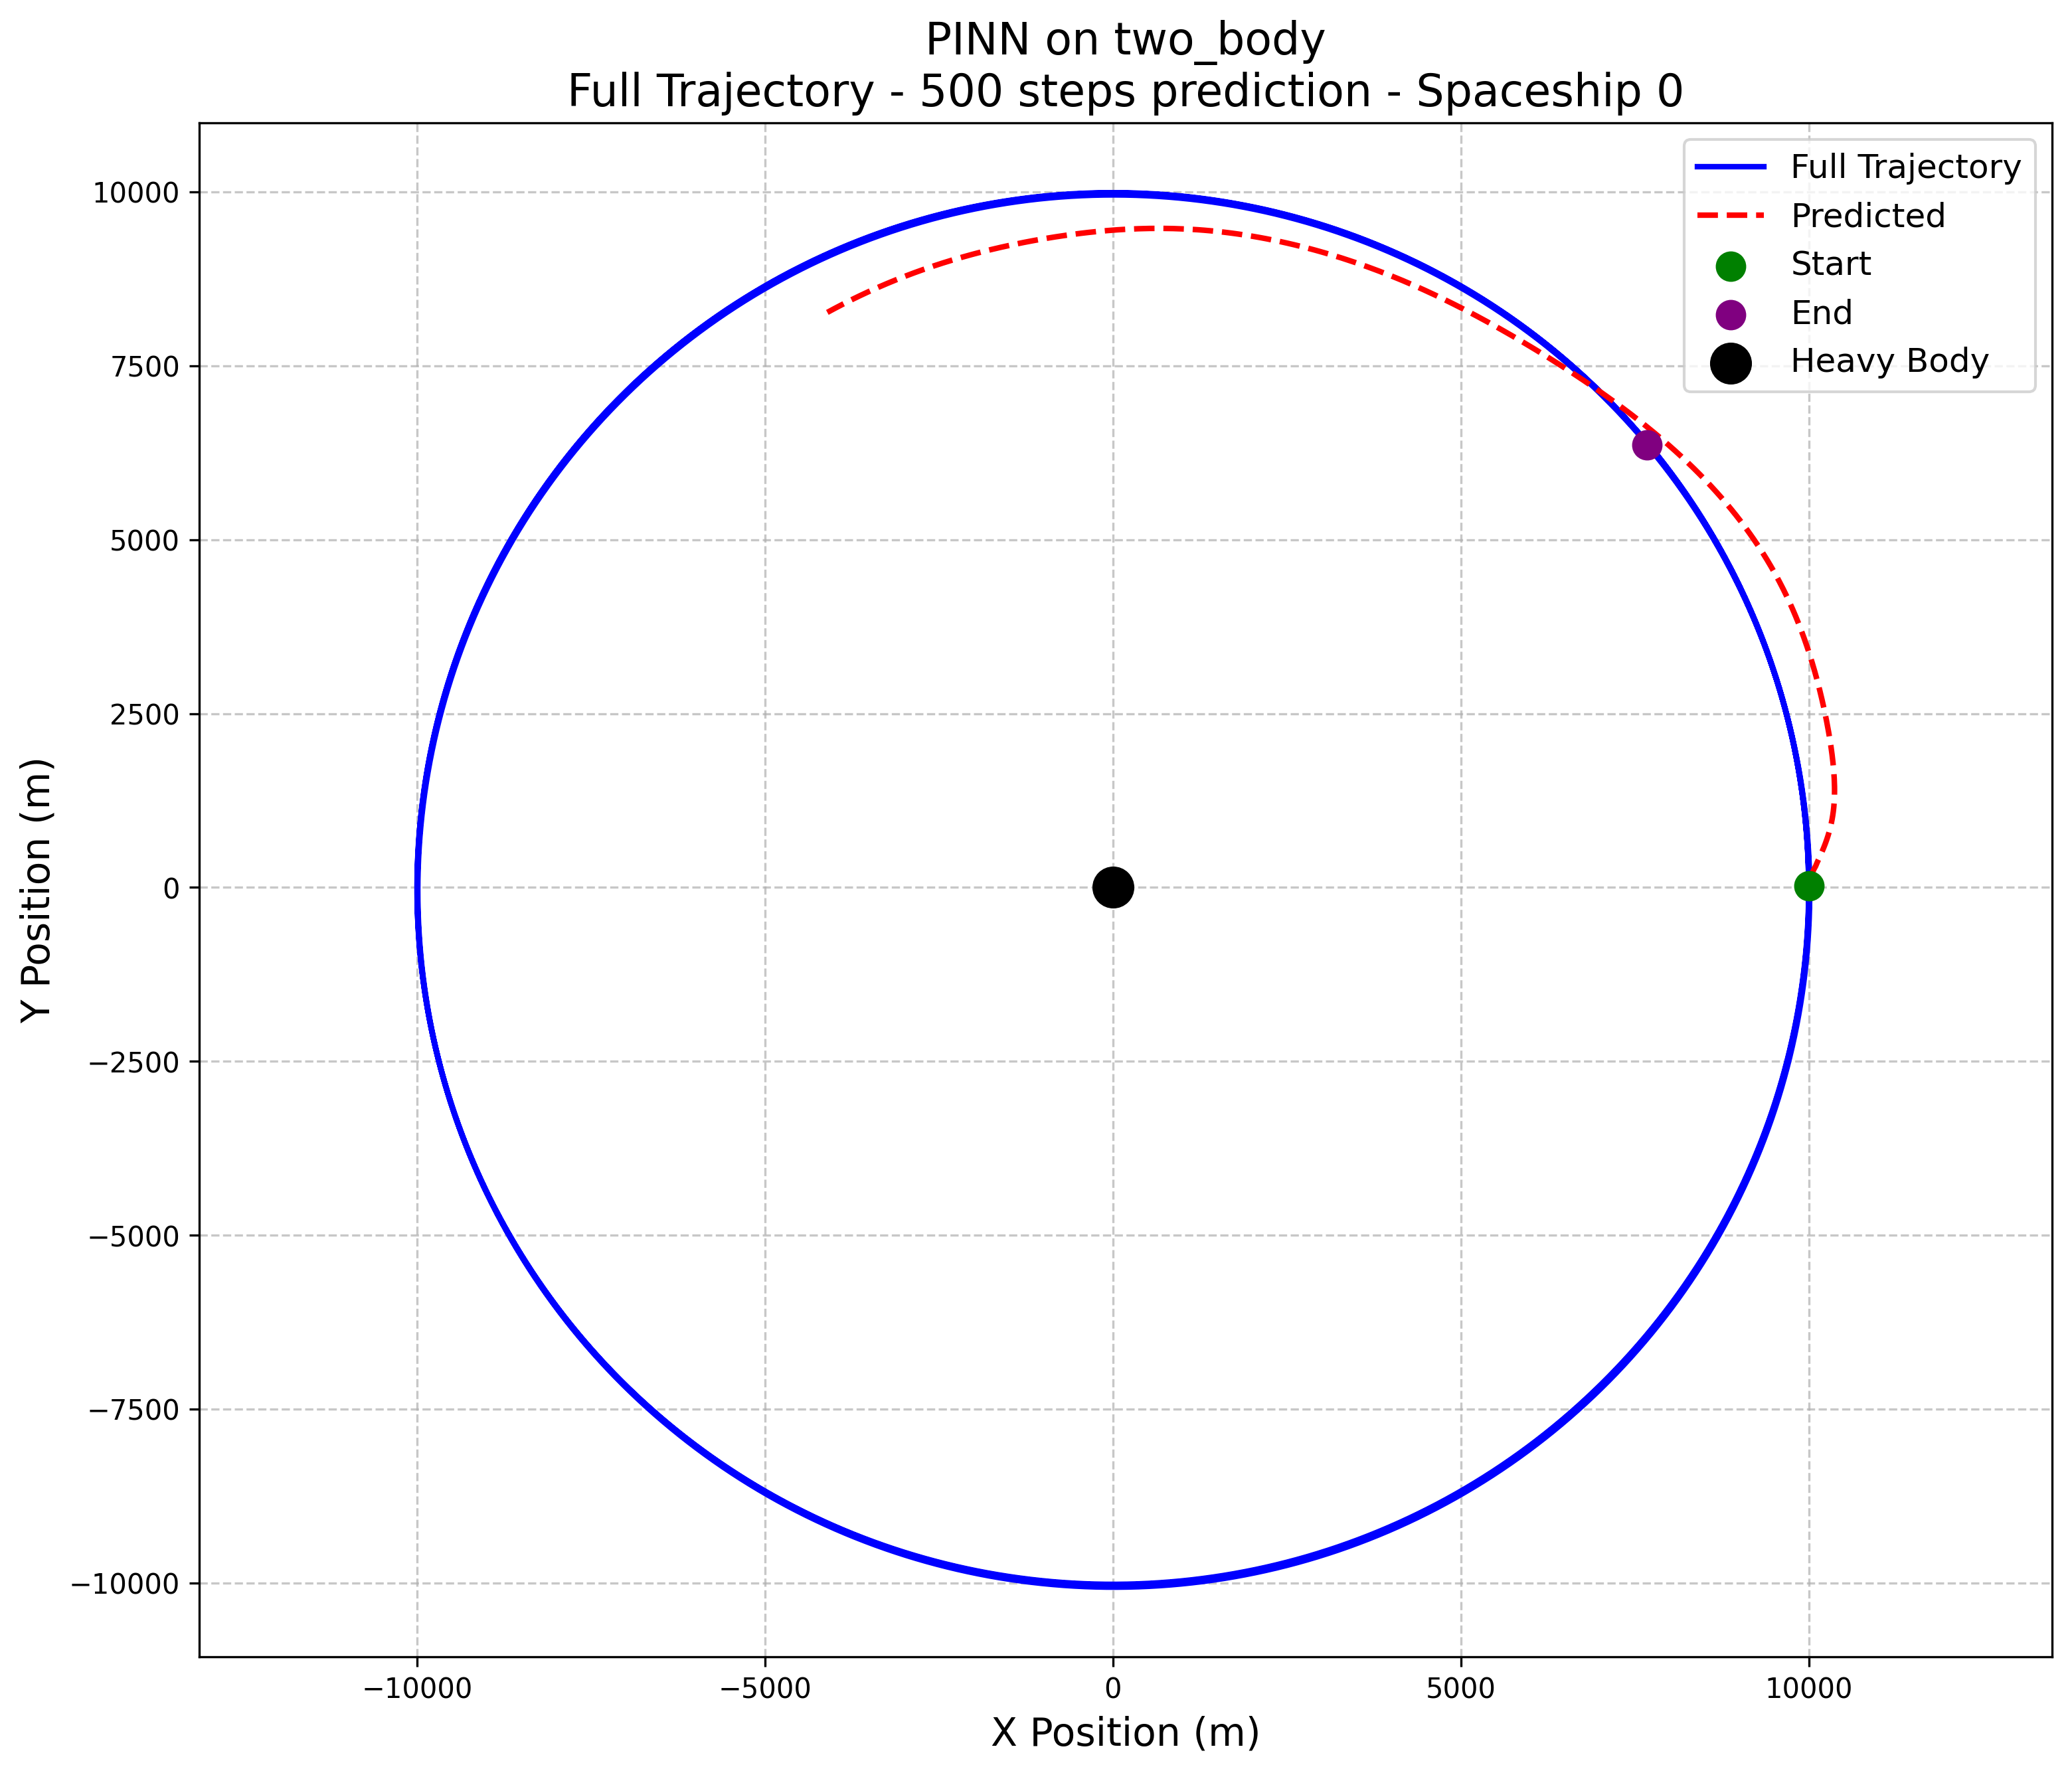
\includegraphics[width=0.27\textwidth]{../inference_results/val/PINN/two_body/500/full_trajectory_spaceship_0.png} &
      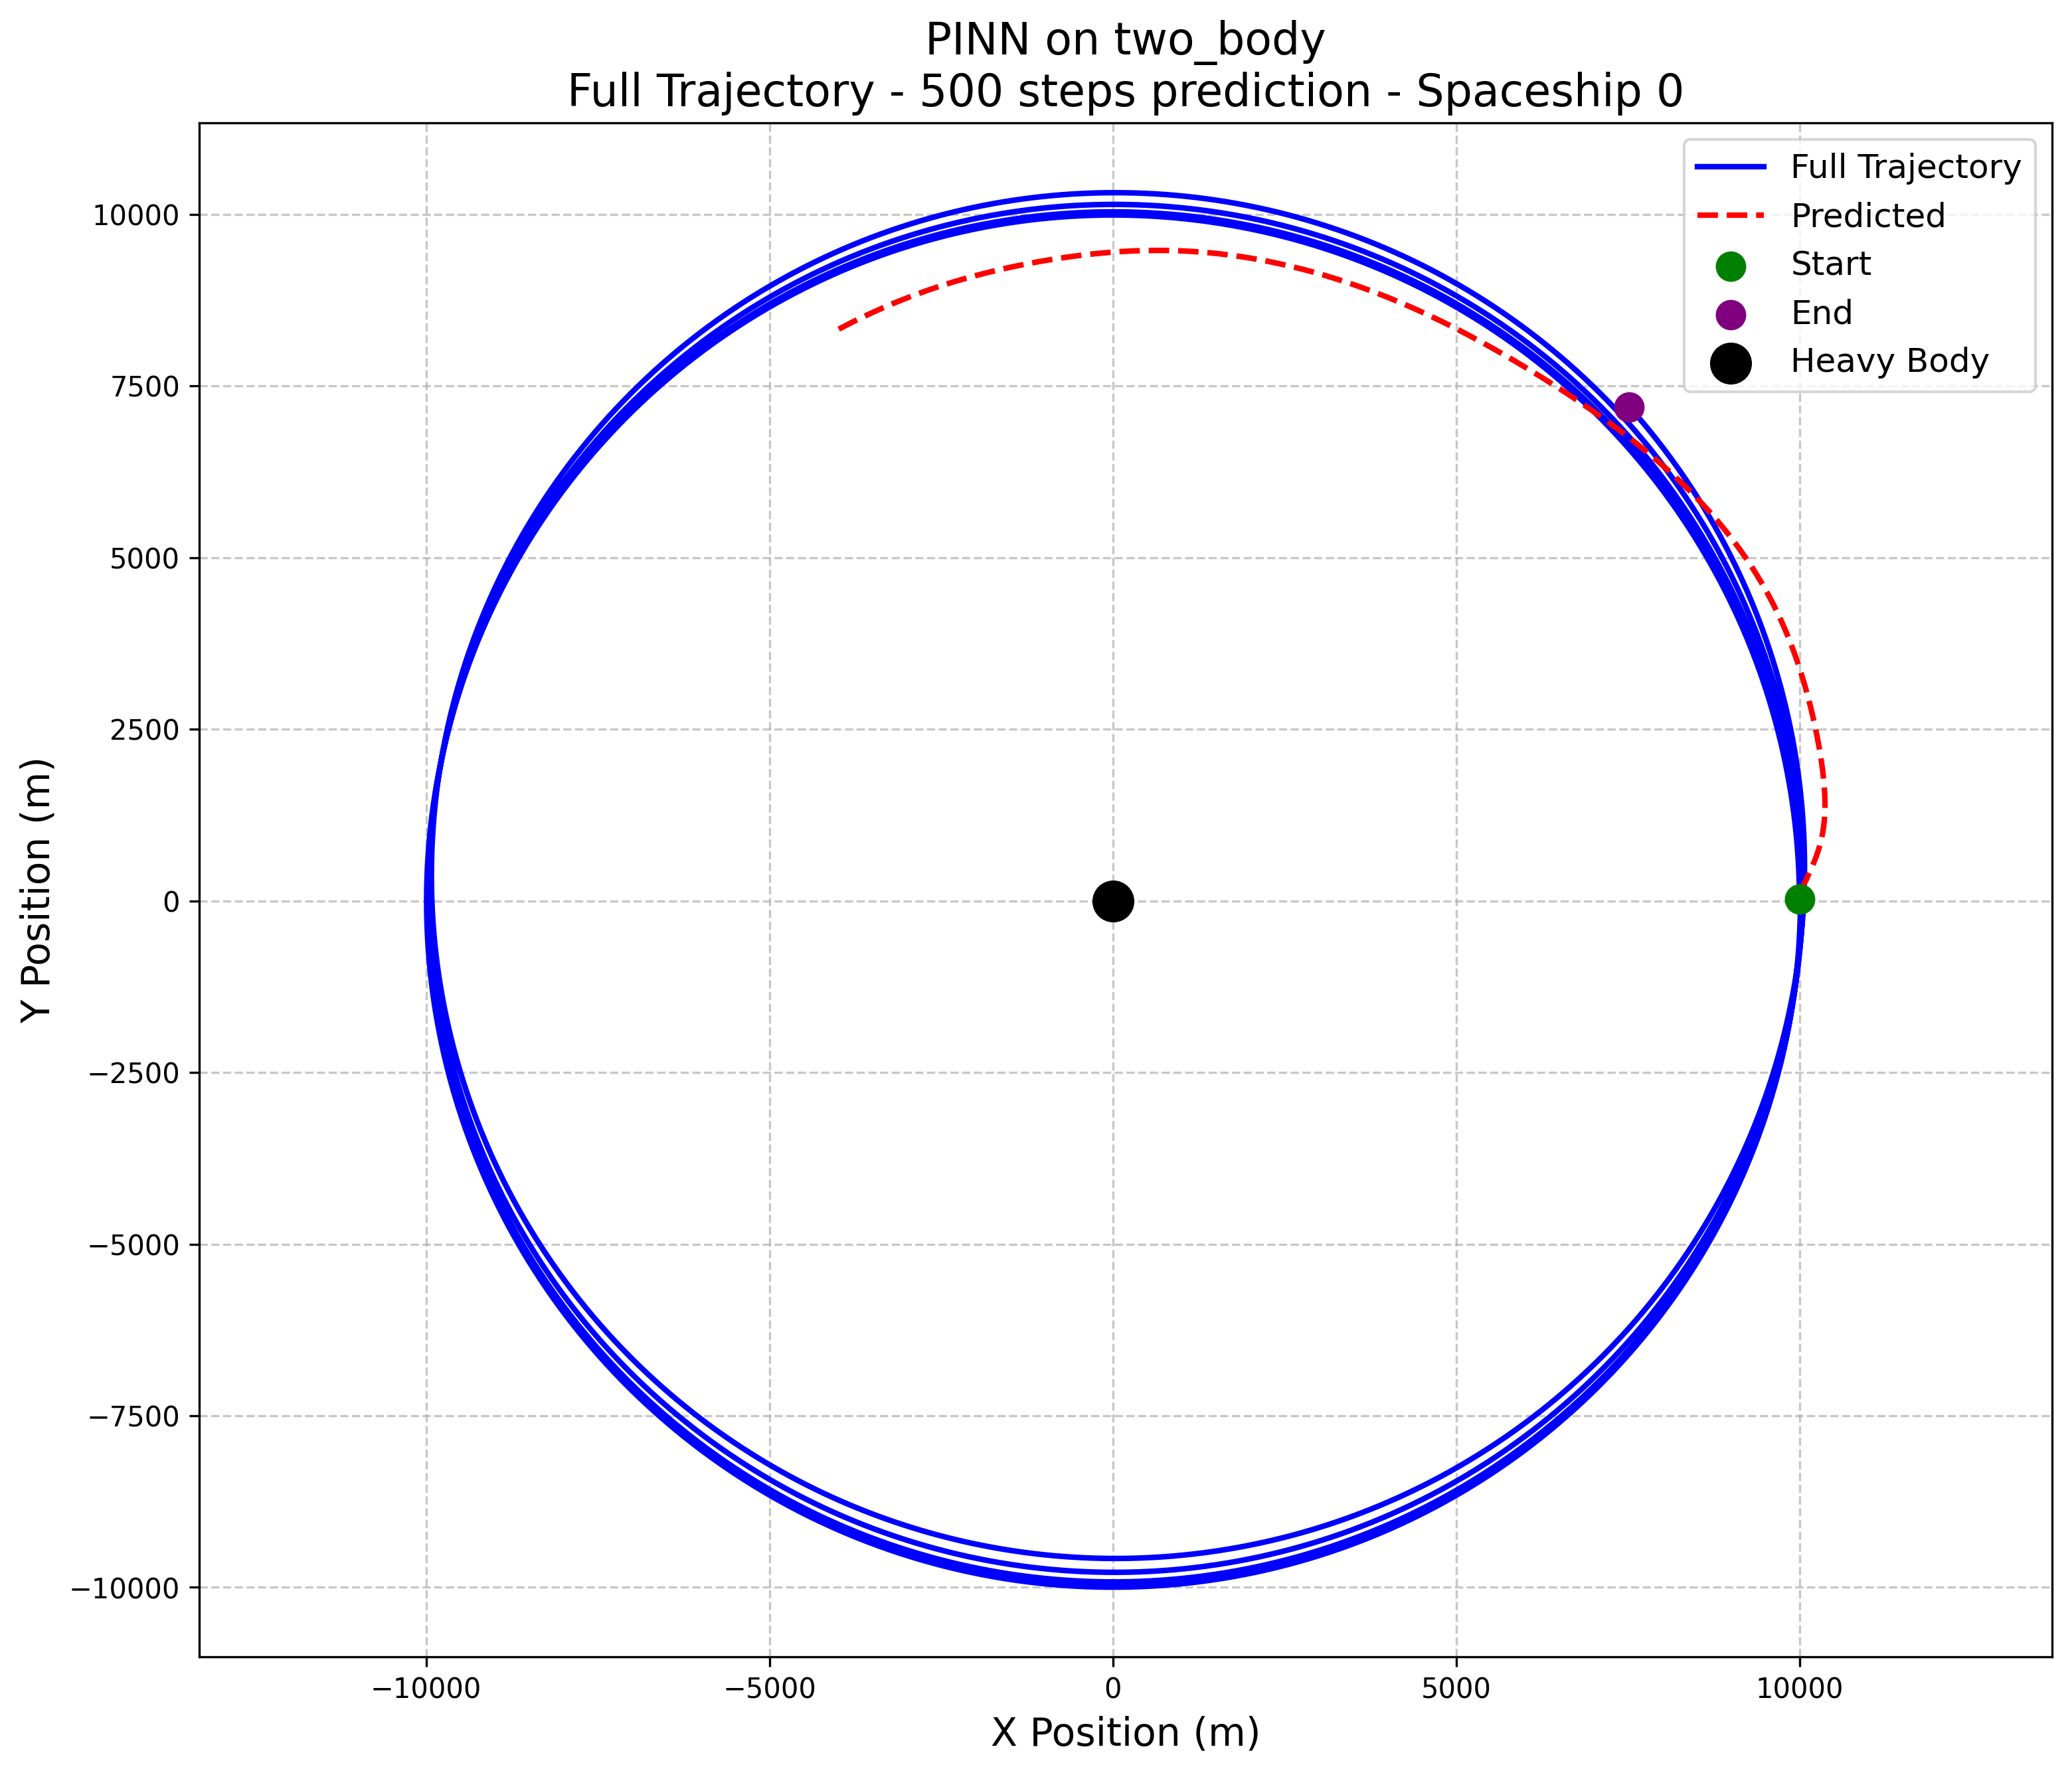
\includegraphics[width=0.27\textwidth]{../inference_results/test/PINN/two_body/500/full_trajectory_spaceship_0.png}
  \end{tabular}
\end{figure}

\section{Two-Body Problem with Increased Acceleration Trajectory Predictions}
\label{sec:two_body_acc_predictions}
\begin{figure}[H]
  \centering
  \caption{Two-Body Problem with Increased Acceleration: Model Predictions vs. Actual Trajectories for first spaceship}
  \label{fig:two_body_acc_predictions}
  \begin{tabular}{cccc}
      & Train & Validation & Test \\
      MLP &
      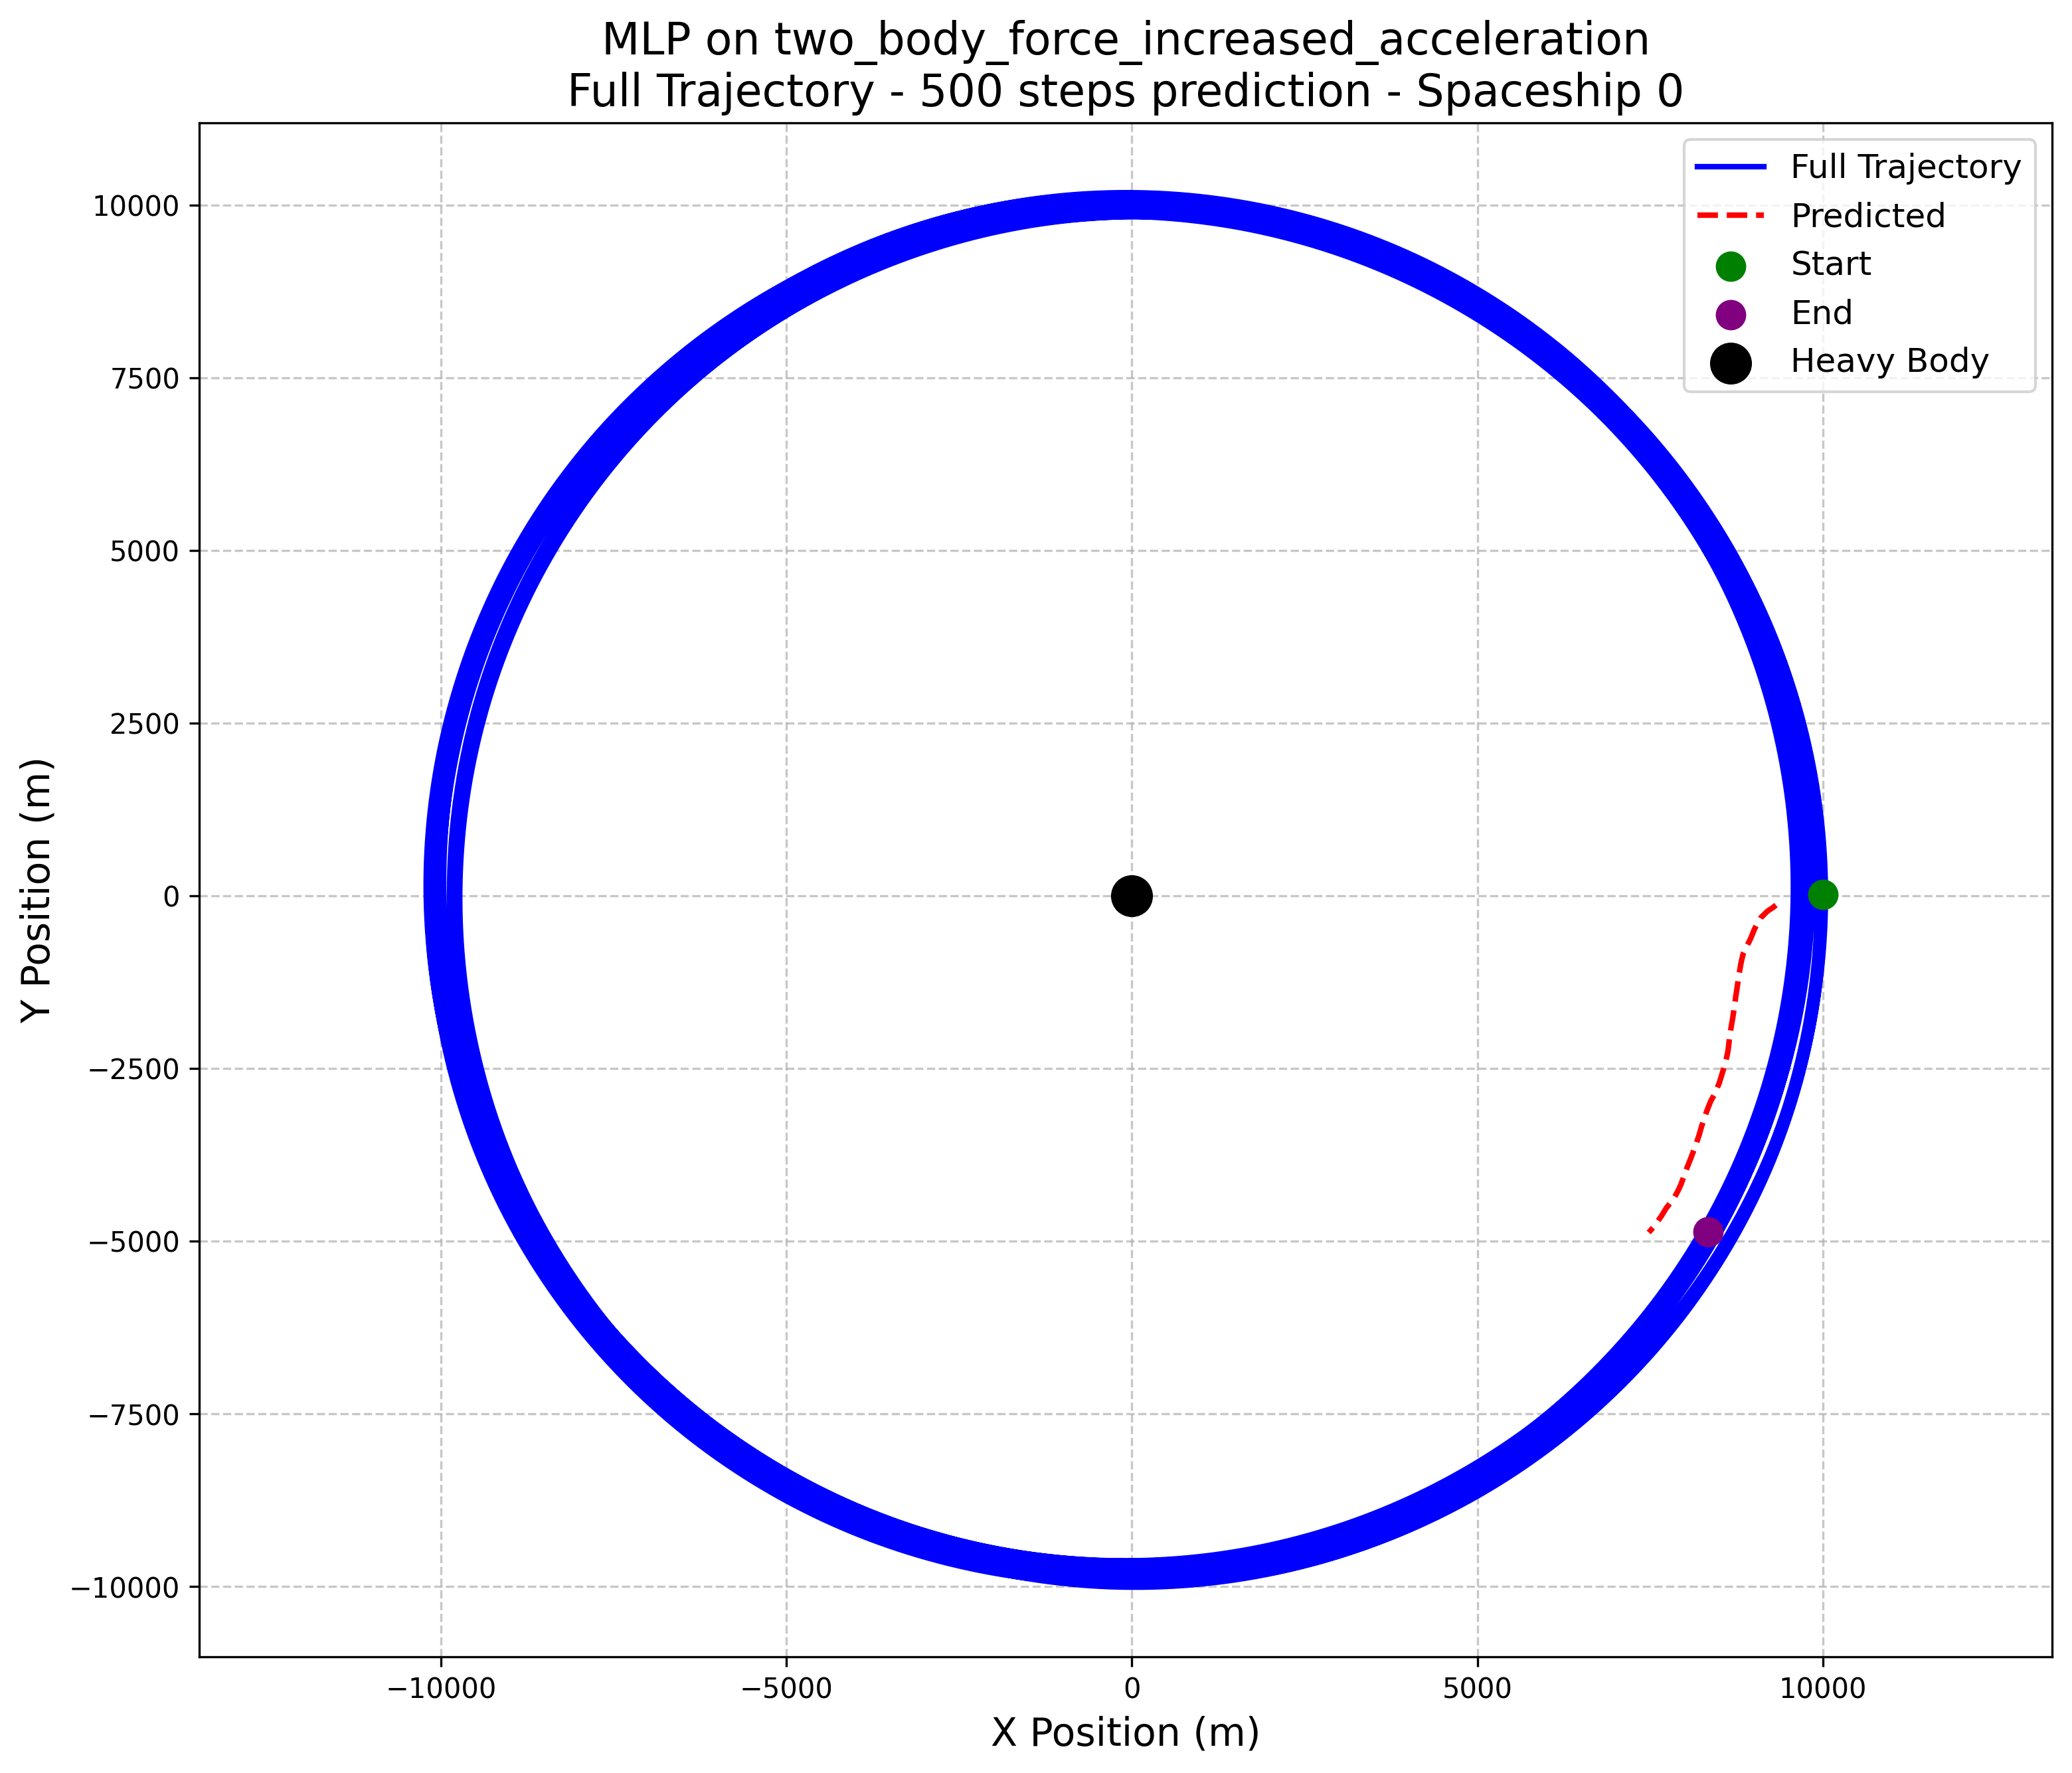
\includegraphics[width=0.27\textwidth]{../inference_results/train/MLP/two_body_force_increased_acceleration/500/full_trajectory_spaceship_0.png} &
      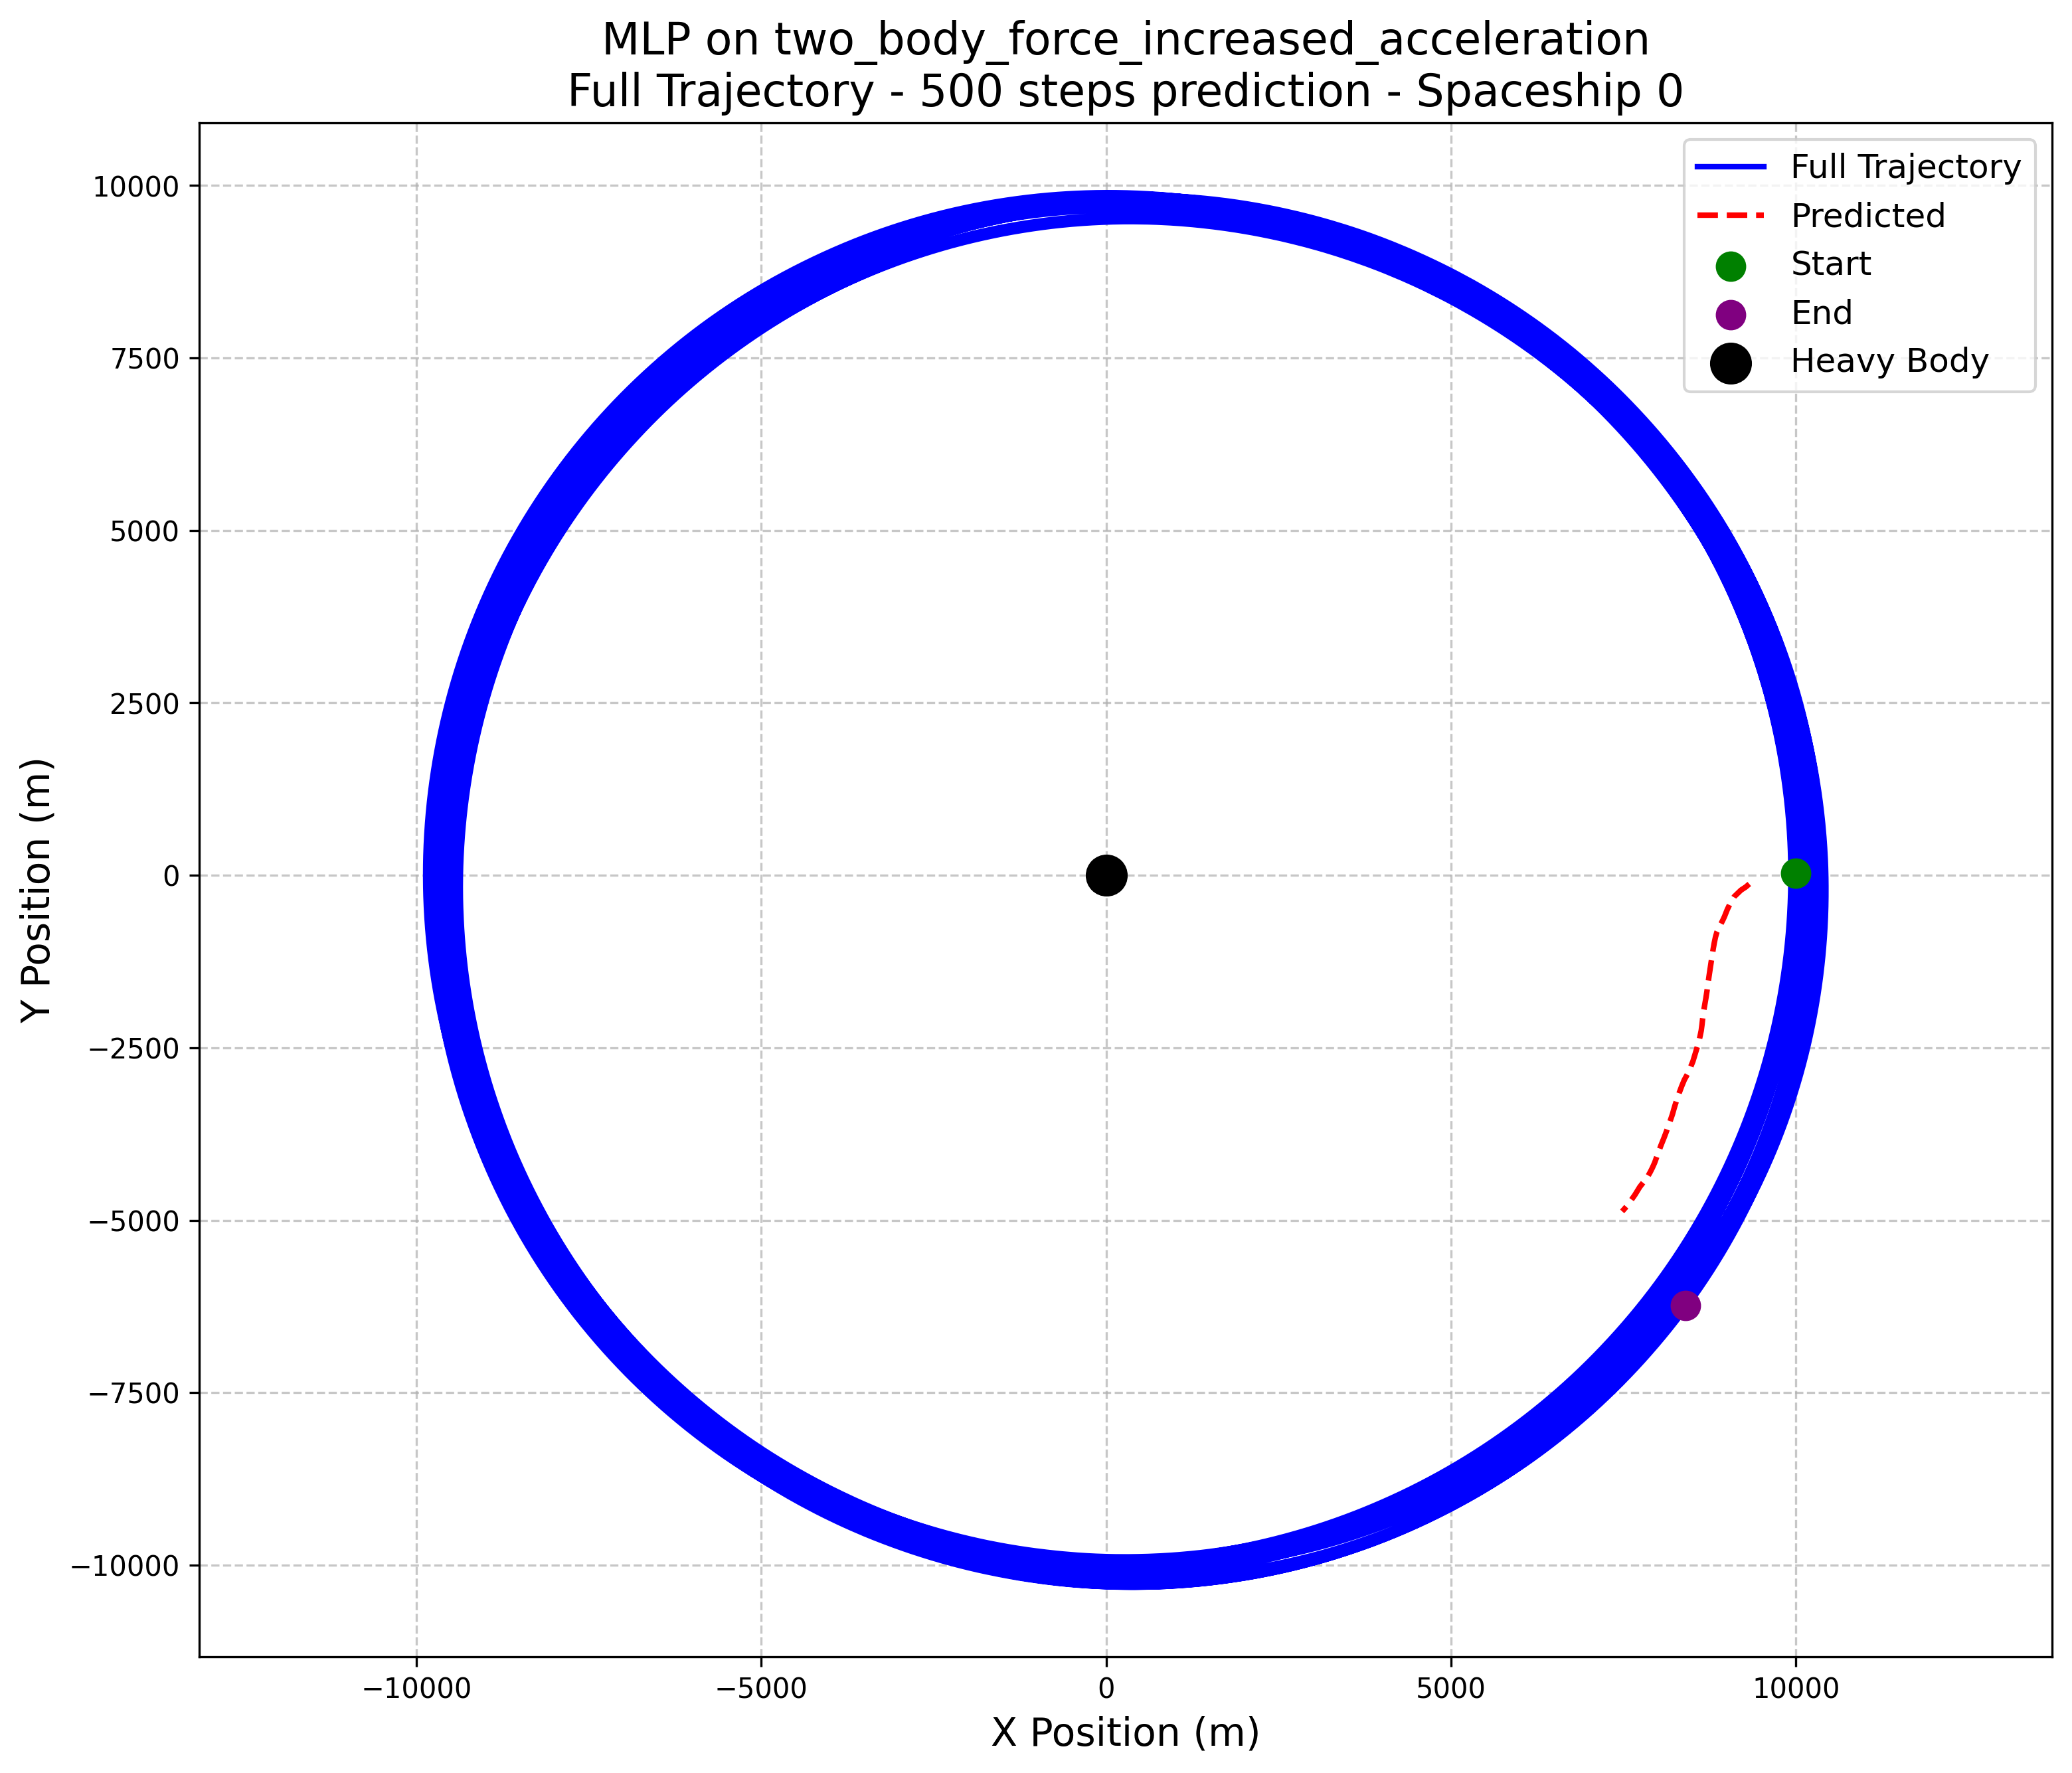
\includegraphics[width=0.27\textwidth]{../inference_results/val/MLP/two_body_force_increased_acceleration/500/full_trajectory_spaceship_0.png} &
      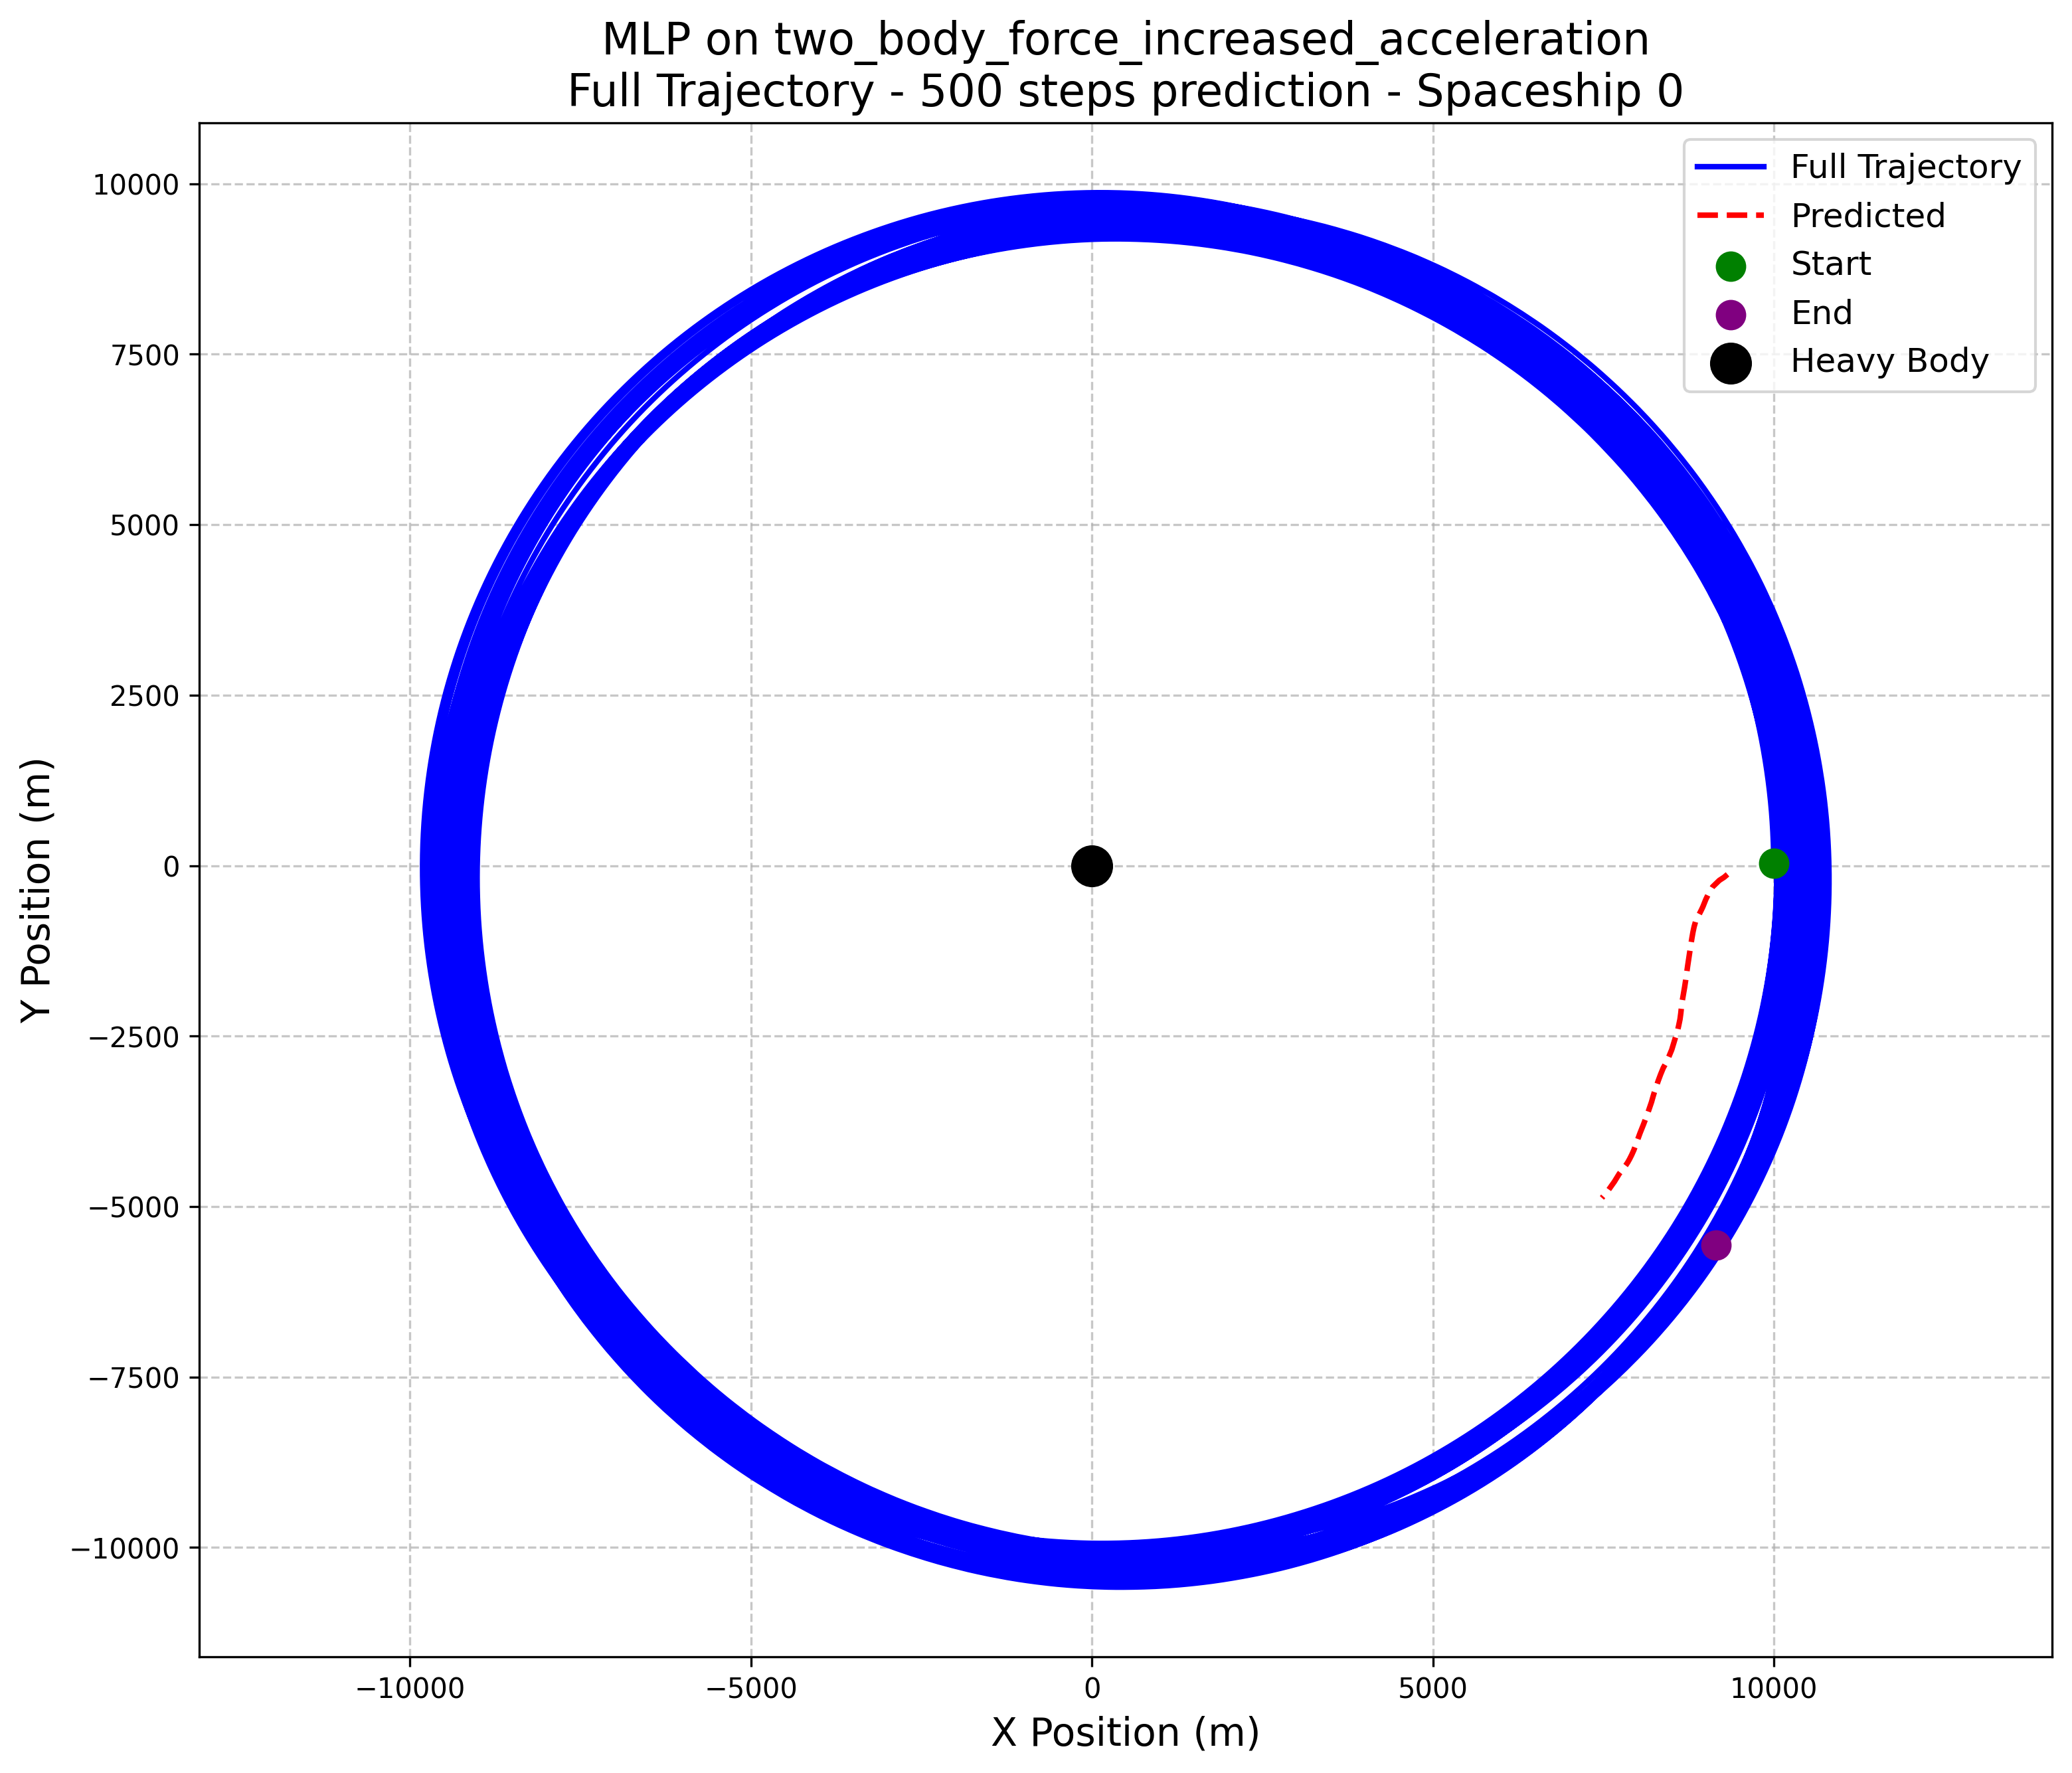
\includegraphics[width=0.27\textwidth]{../inference_results/test/MLP/two_body_force_increased_acceleration/500/full_trajectory_spaceship_0.png} \\
      LSTM &
      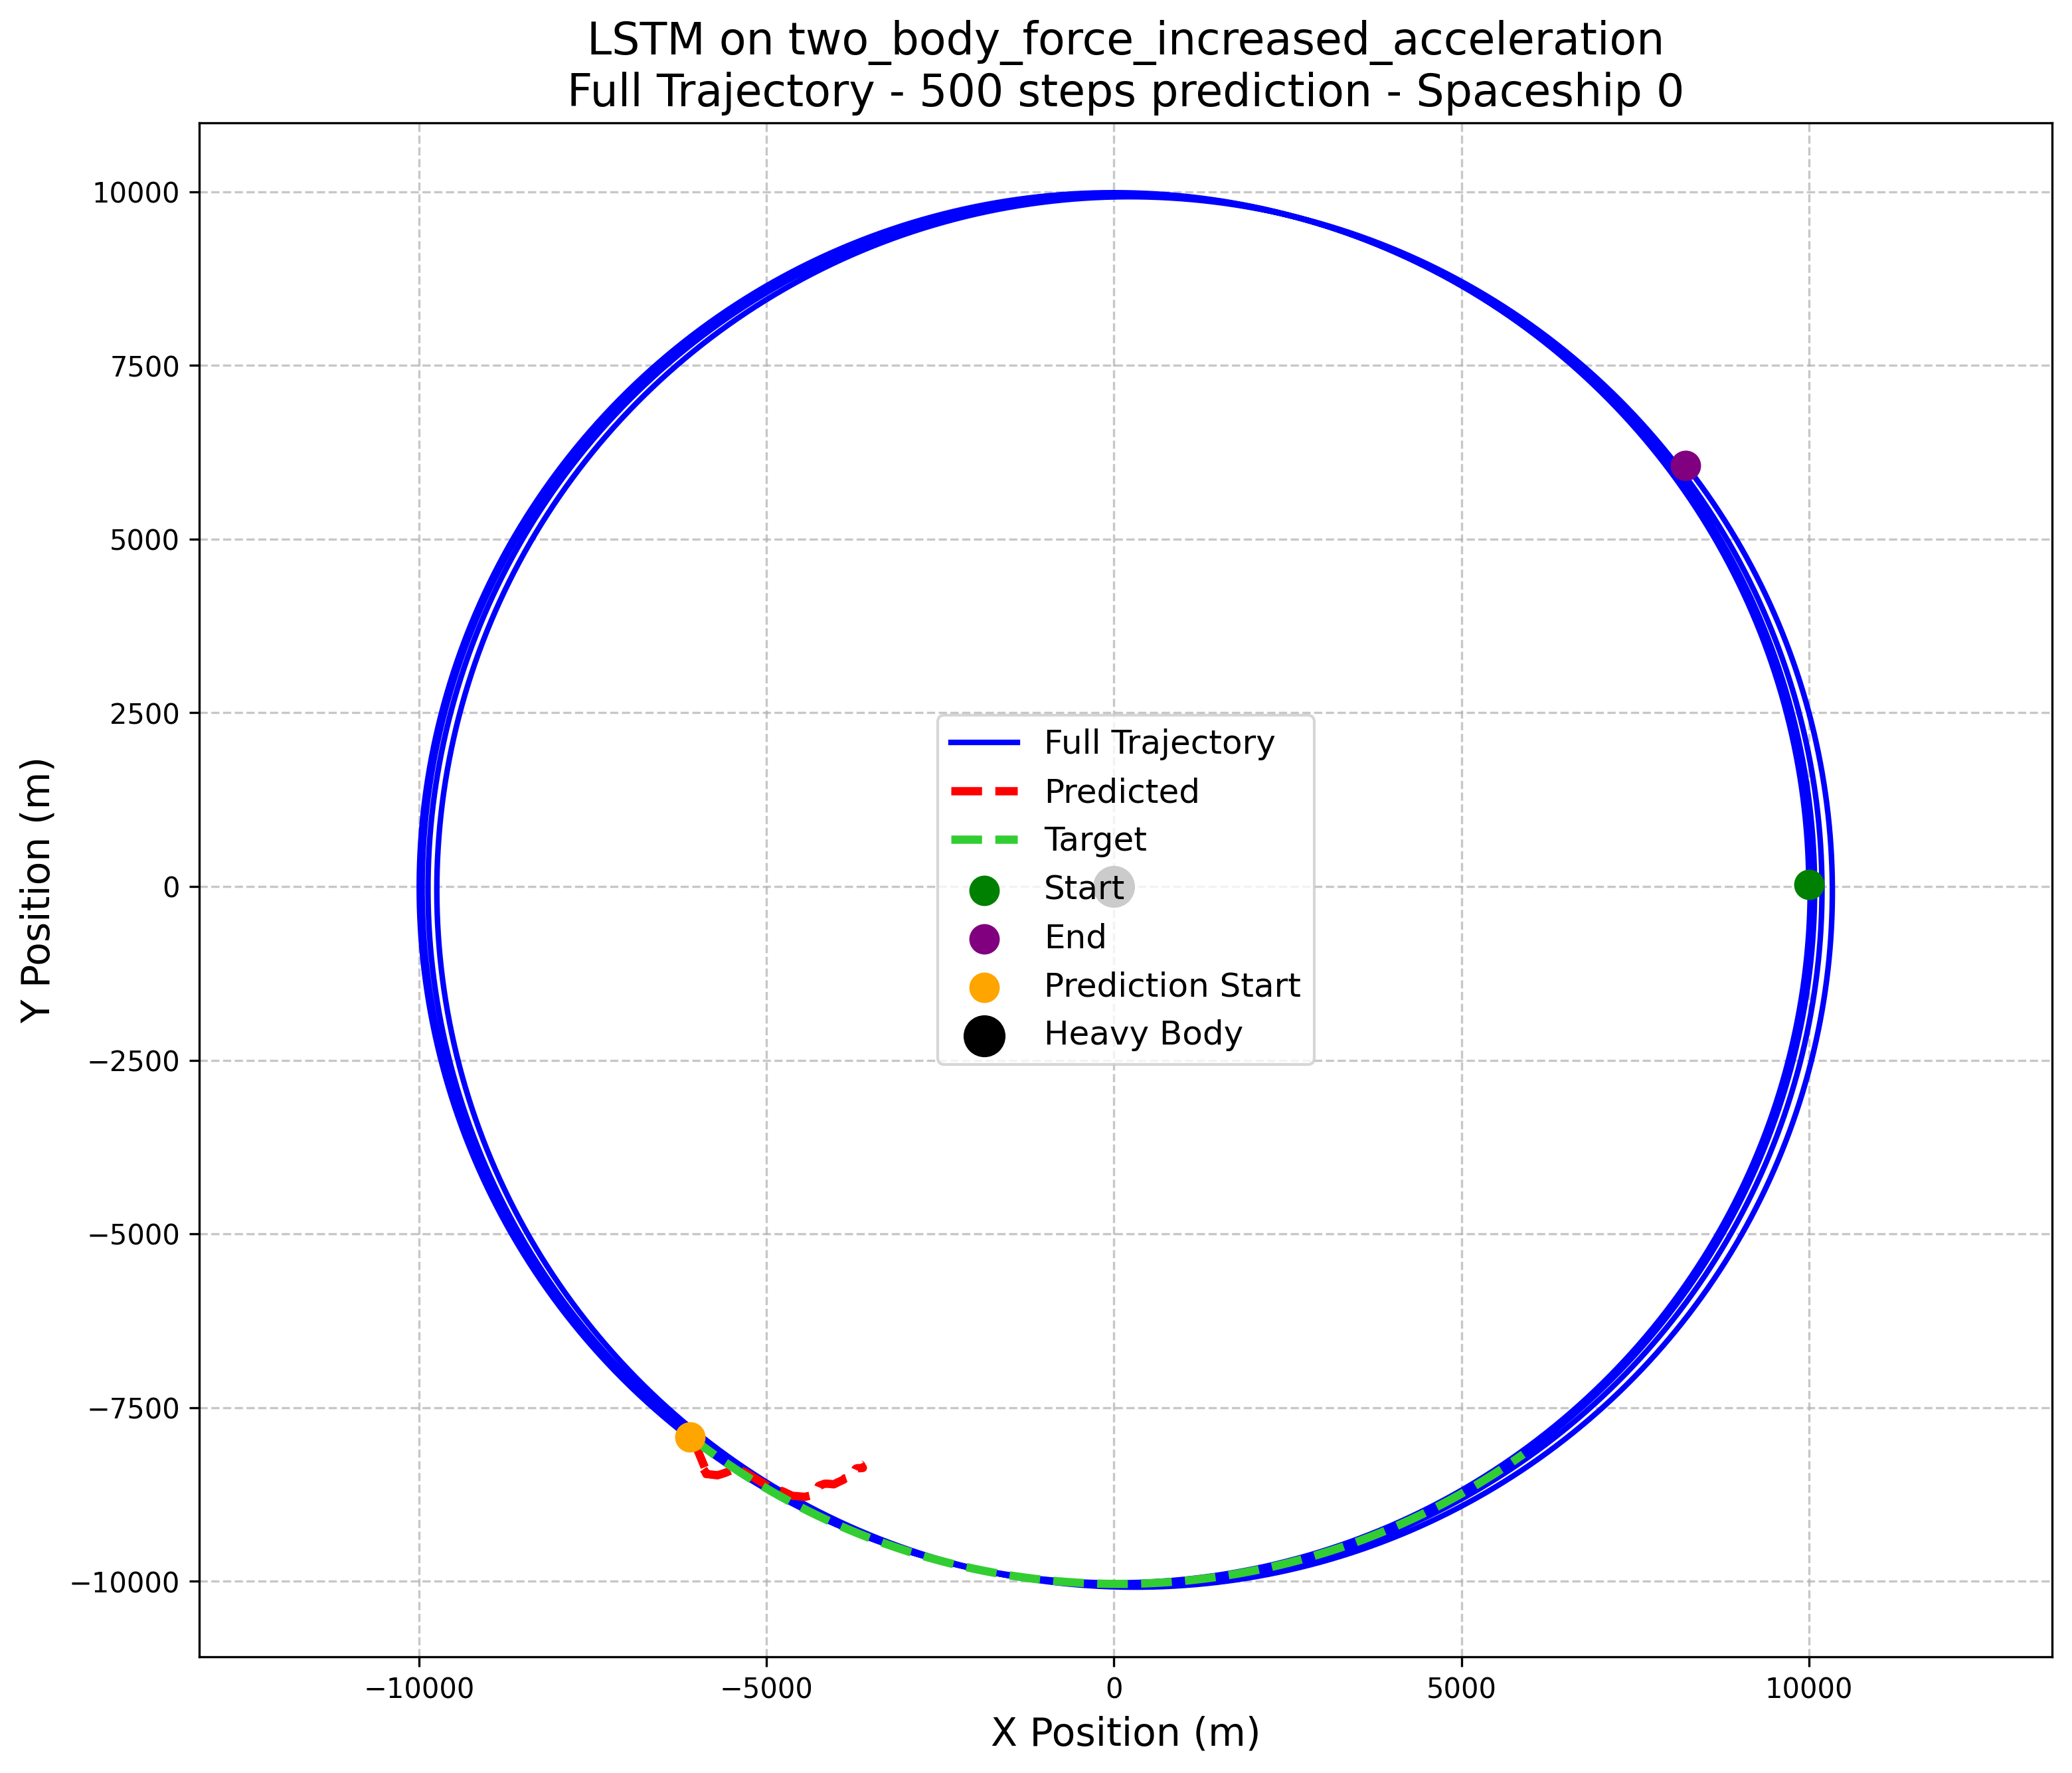
\includegraphics[width=0.27\textwidth]{../inference_results/train/LSTM/two_body_force_increased_acceleration/500/full_trajectory_spaceship_0.png} &
      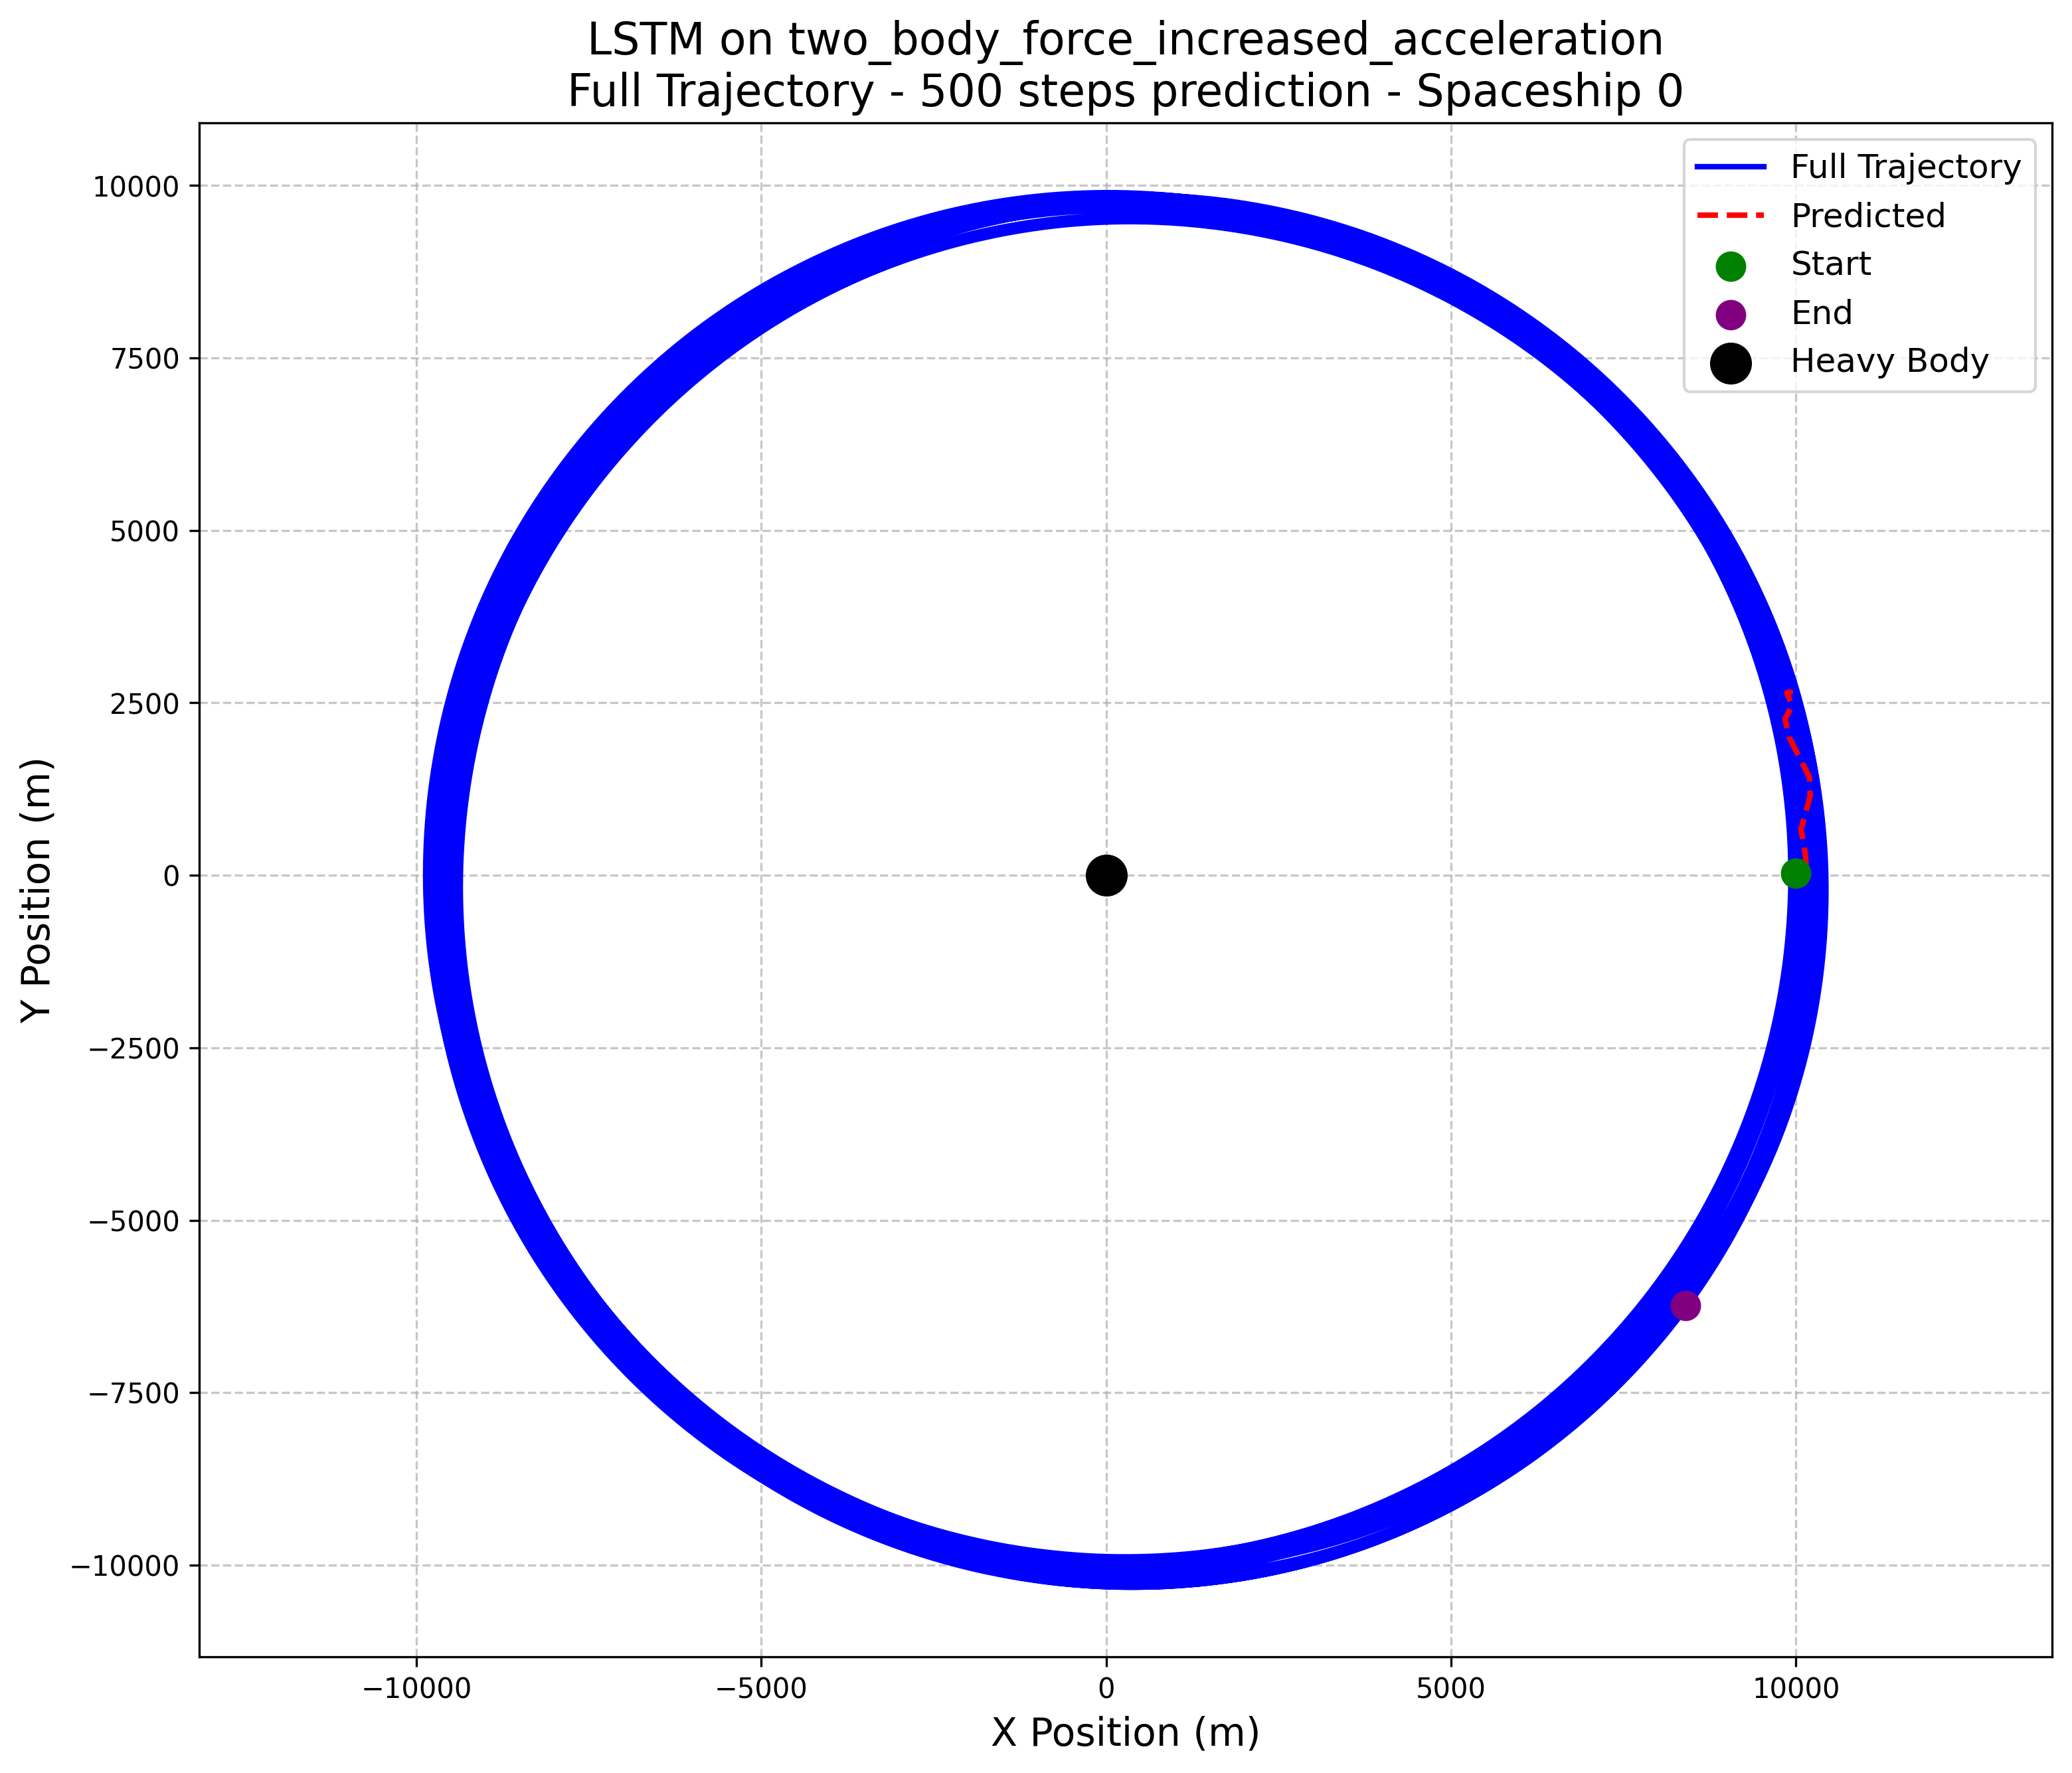
\includegraphics[width=0.27\textwidth]{../inference_results/val/LSTM/two_body_force_increased_acceleration/500/full_trajectory_spaceship_0.png} &
      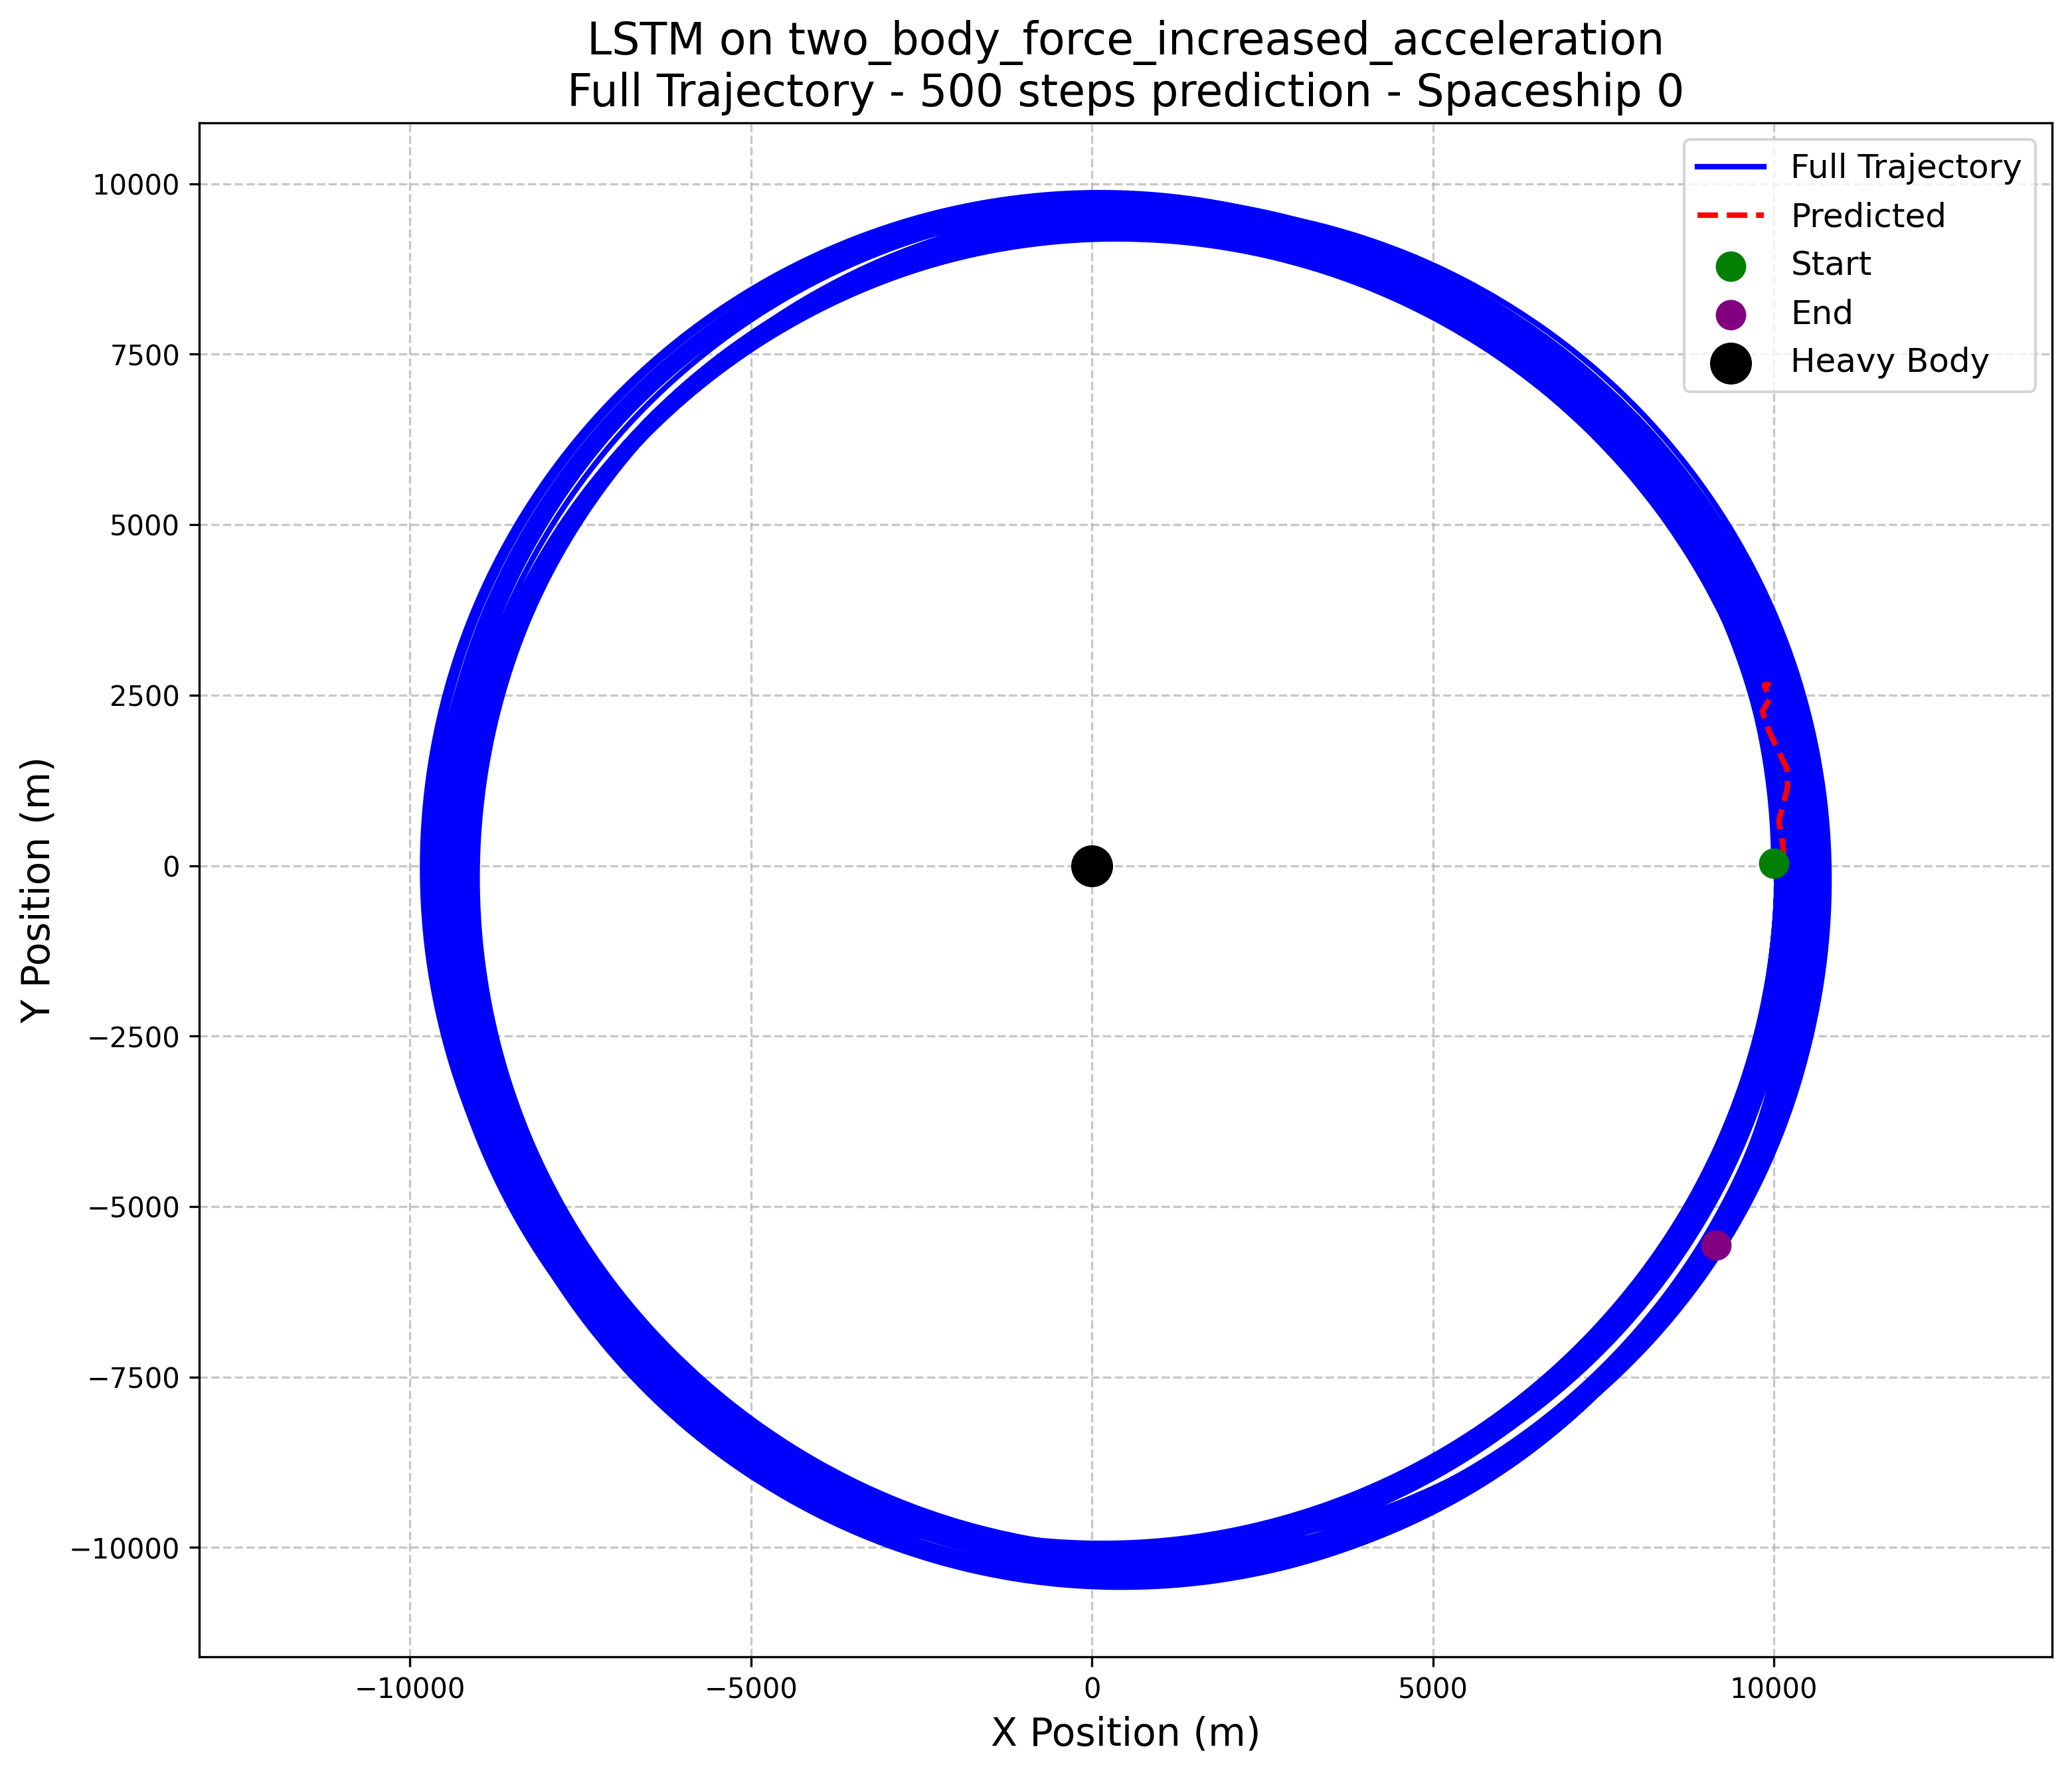
\includegraphics[width=0.27\textwidth]{../inference_results/test/LSTM/two_body_force_increased_acceleration/500/full_trajectory_spaceship_0.png} \\
      PINN &
      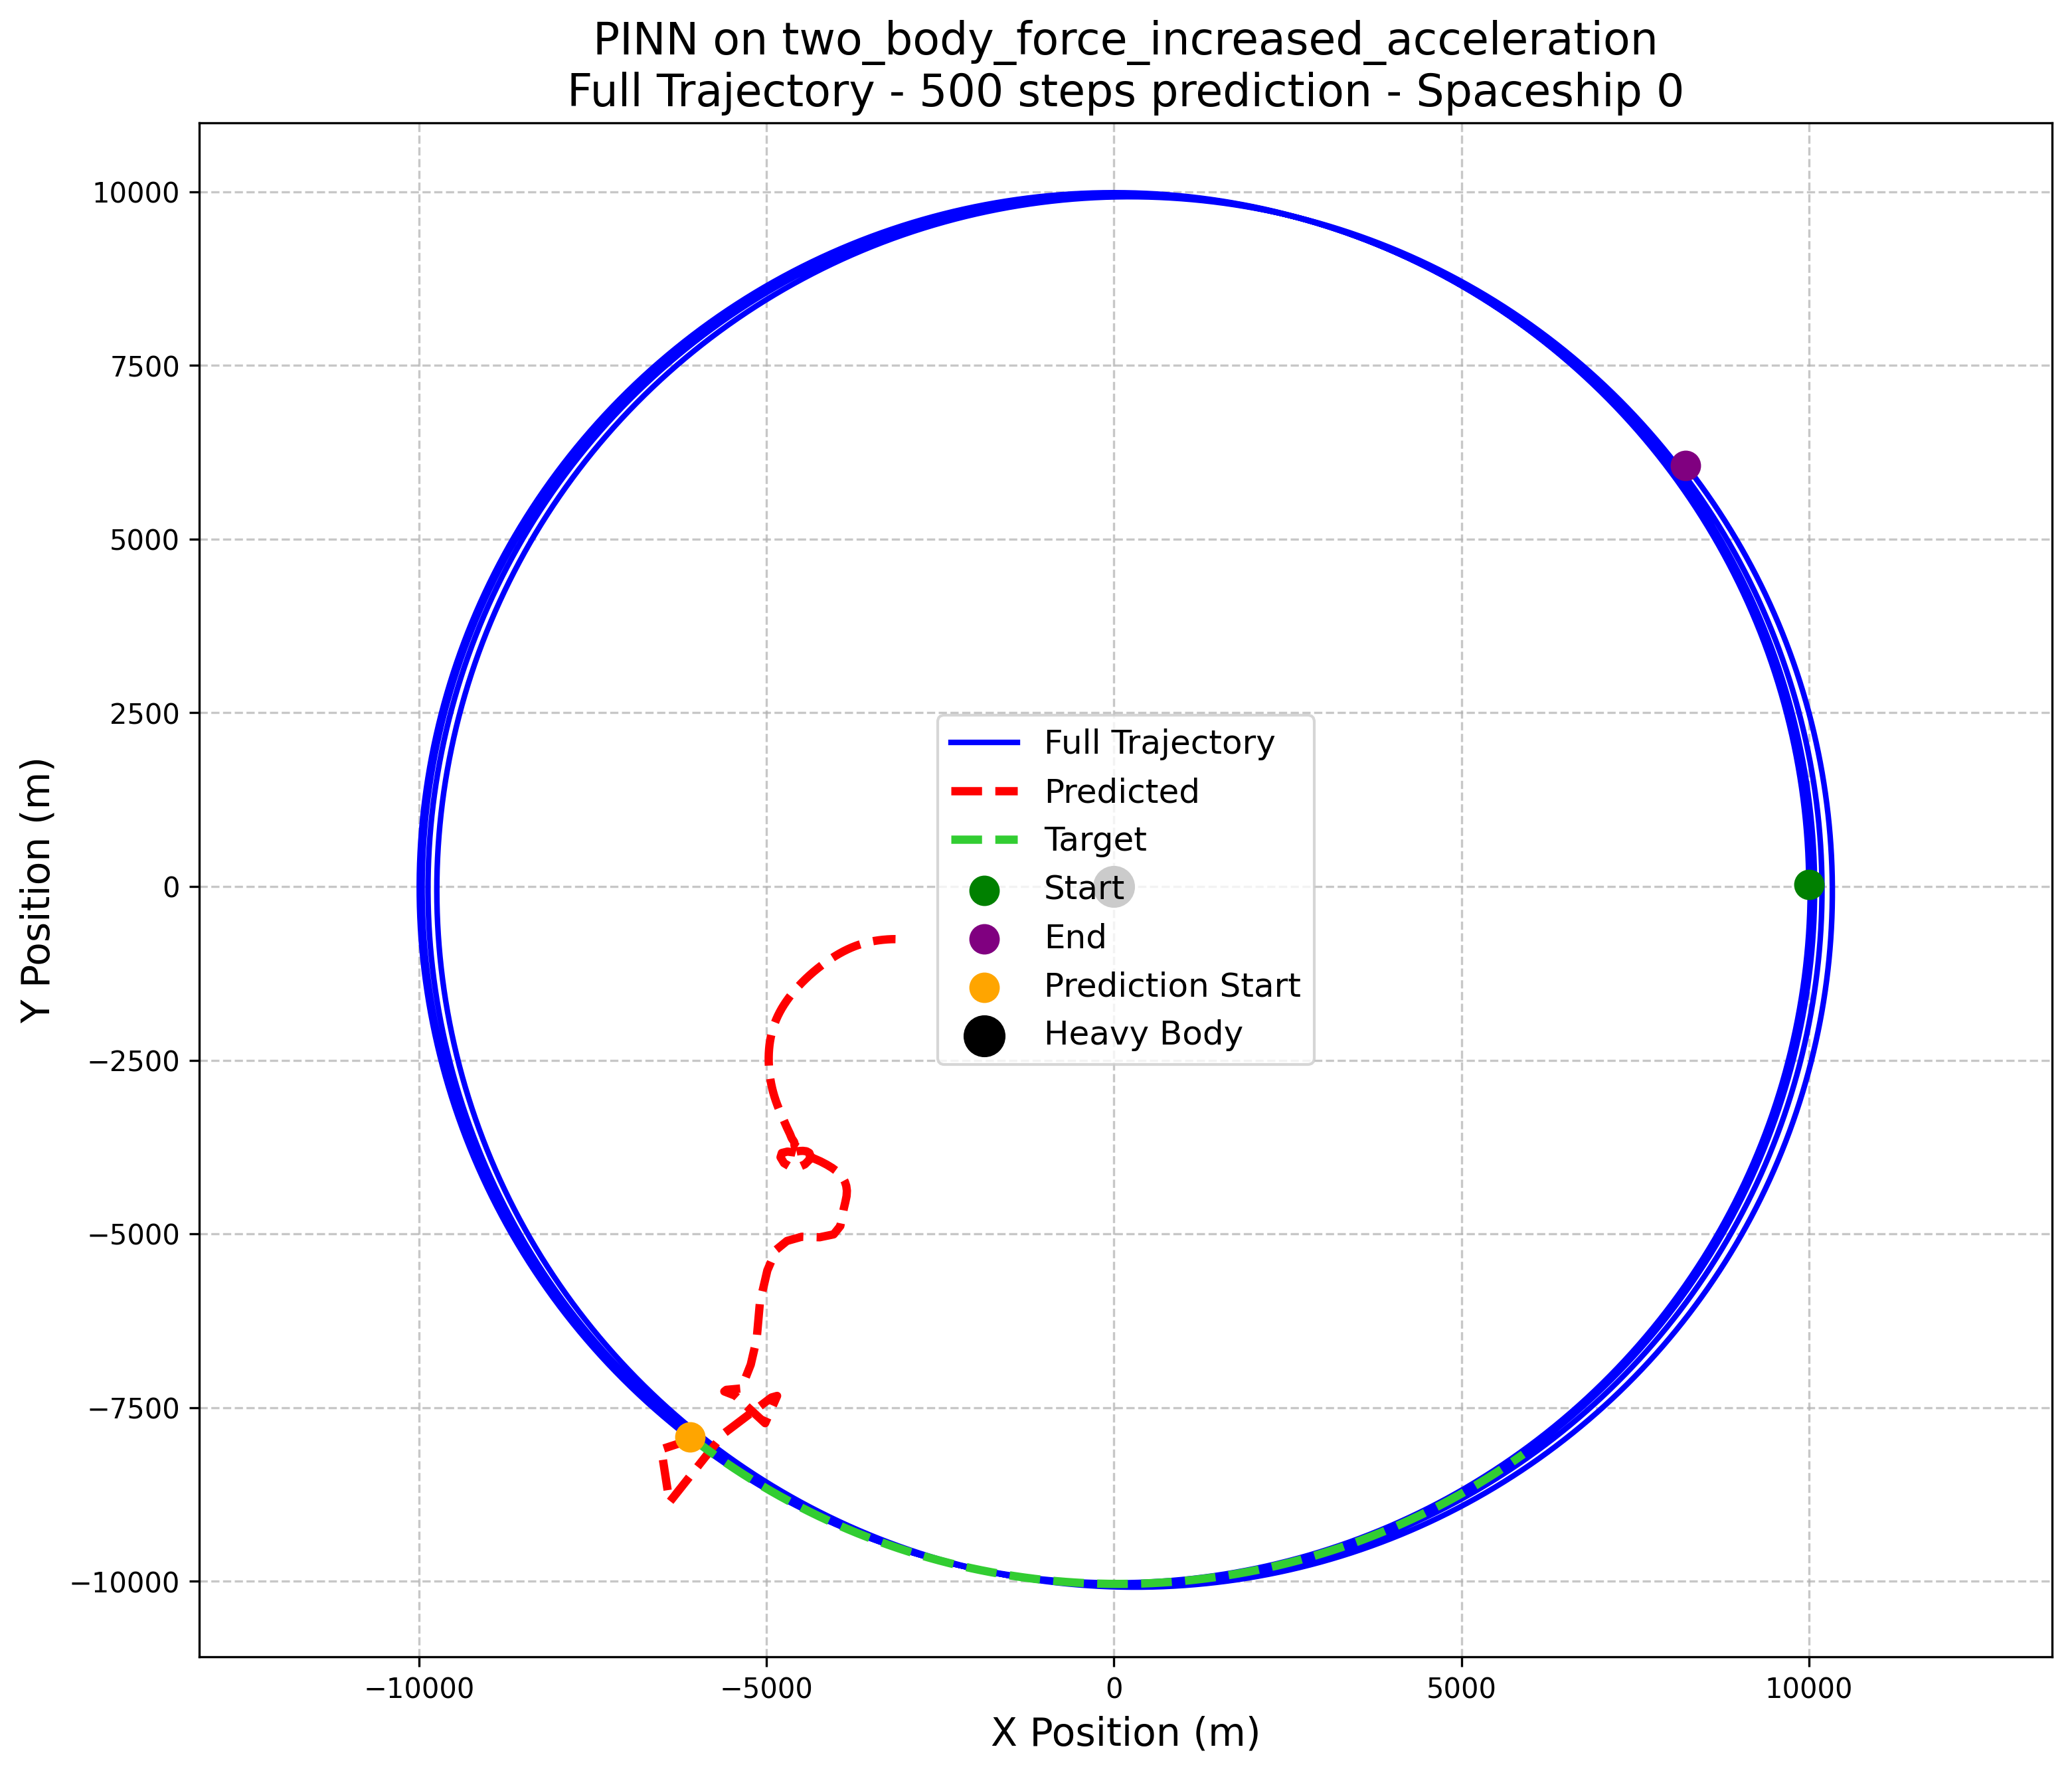
\includegraphics[width=0.27\textwidth]{../inference_results/train/PINN/two_body_force_increased_acceleration/500/full_trajectory_spaceship_0.png} &
      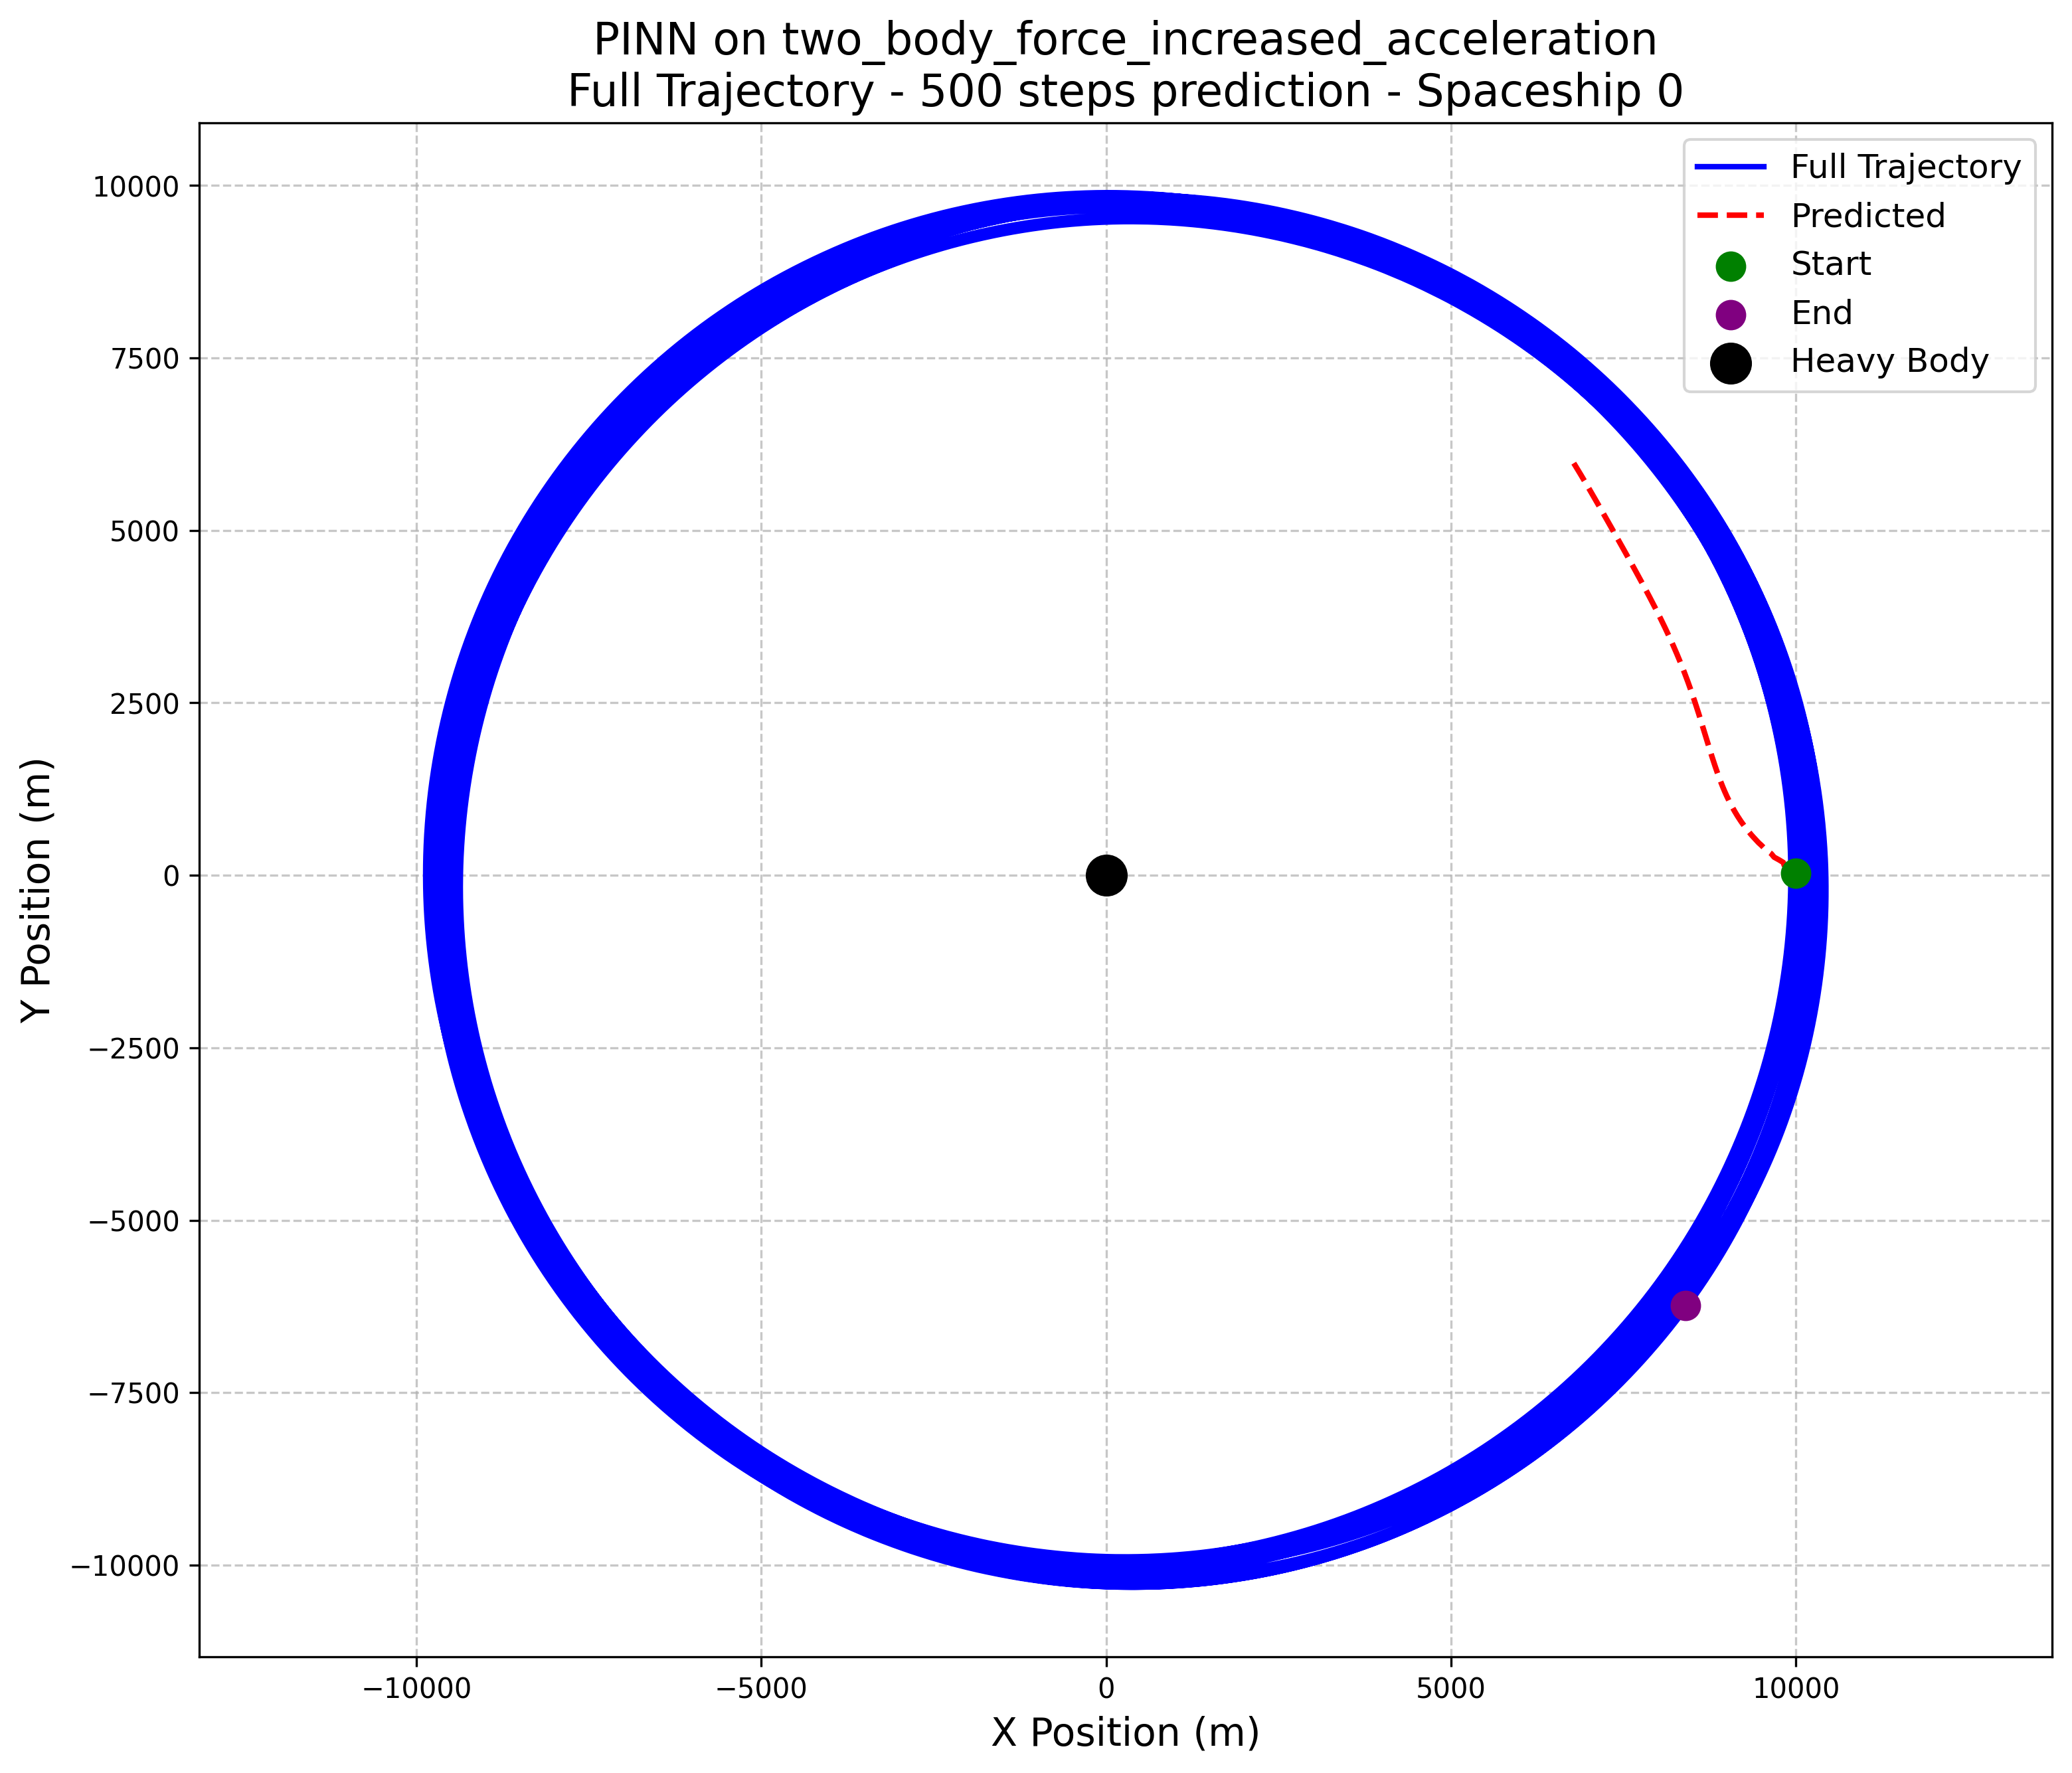
\includegraphics[width=0.27\textwidth]{../inference_results/val/PINN/two_body_force_increased_acceleration/500/full_trajectory_spaceship_0.png} &
      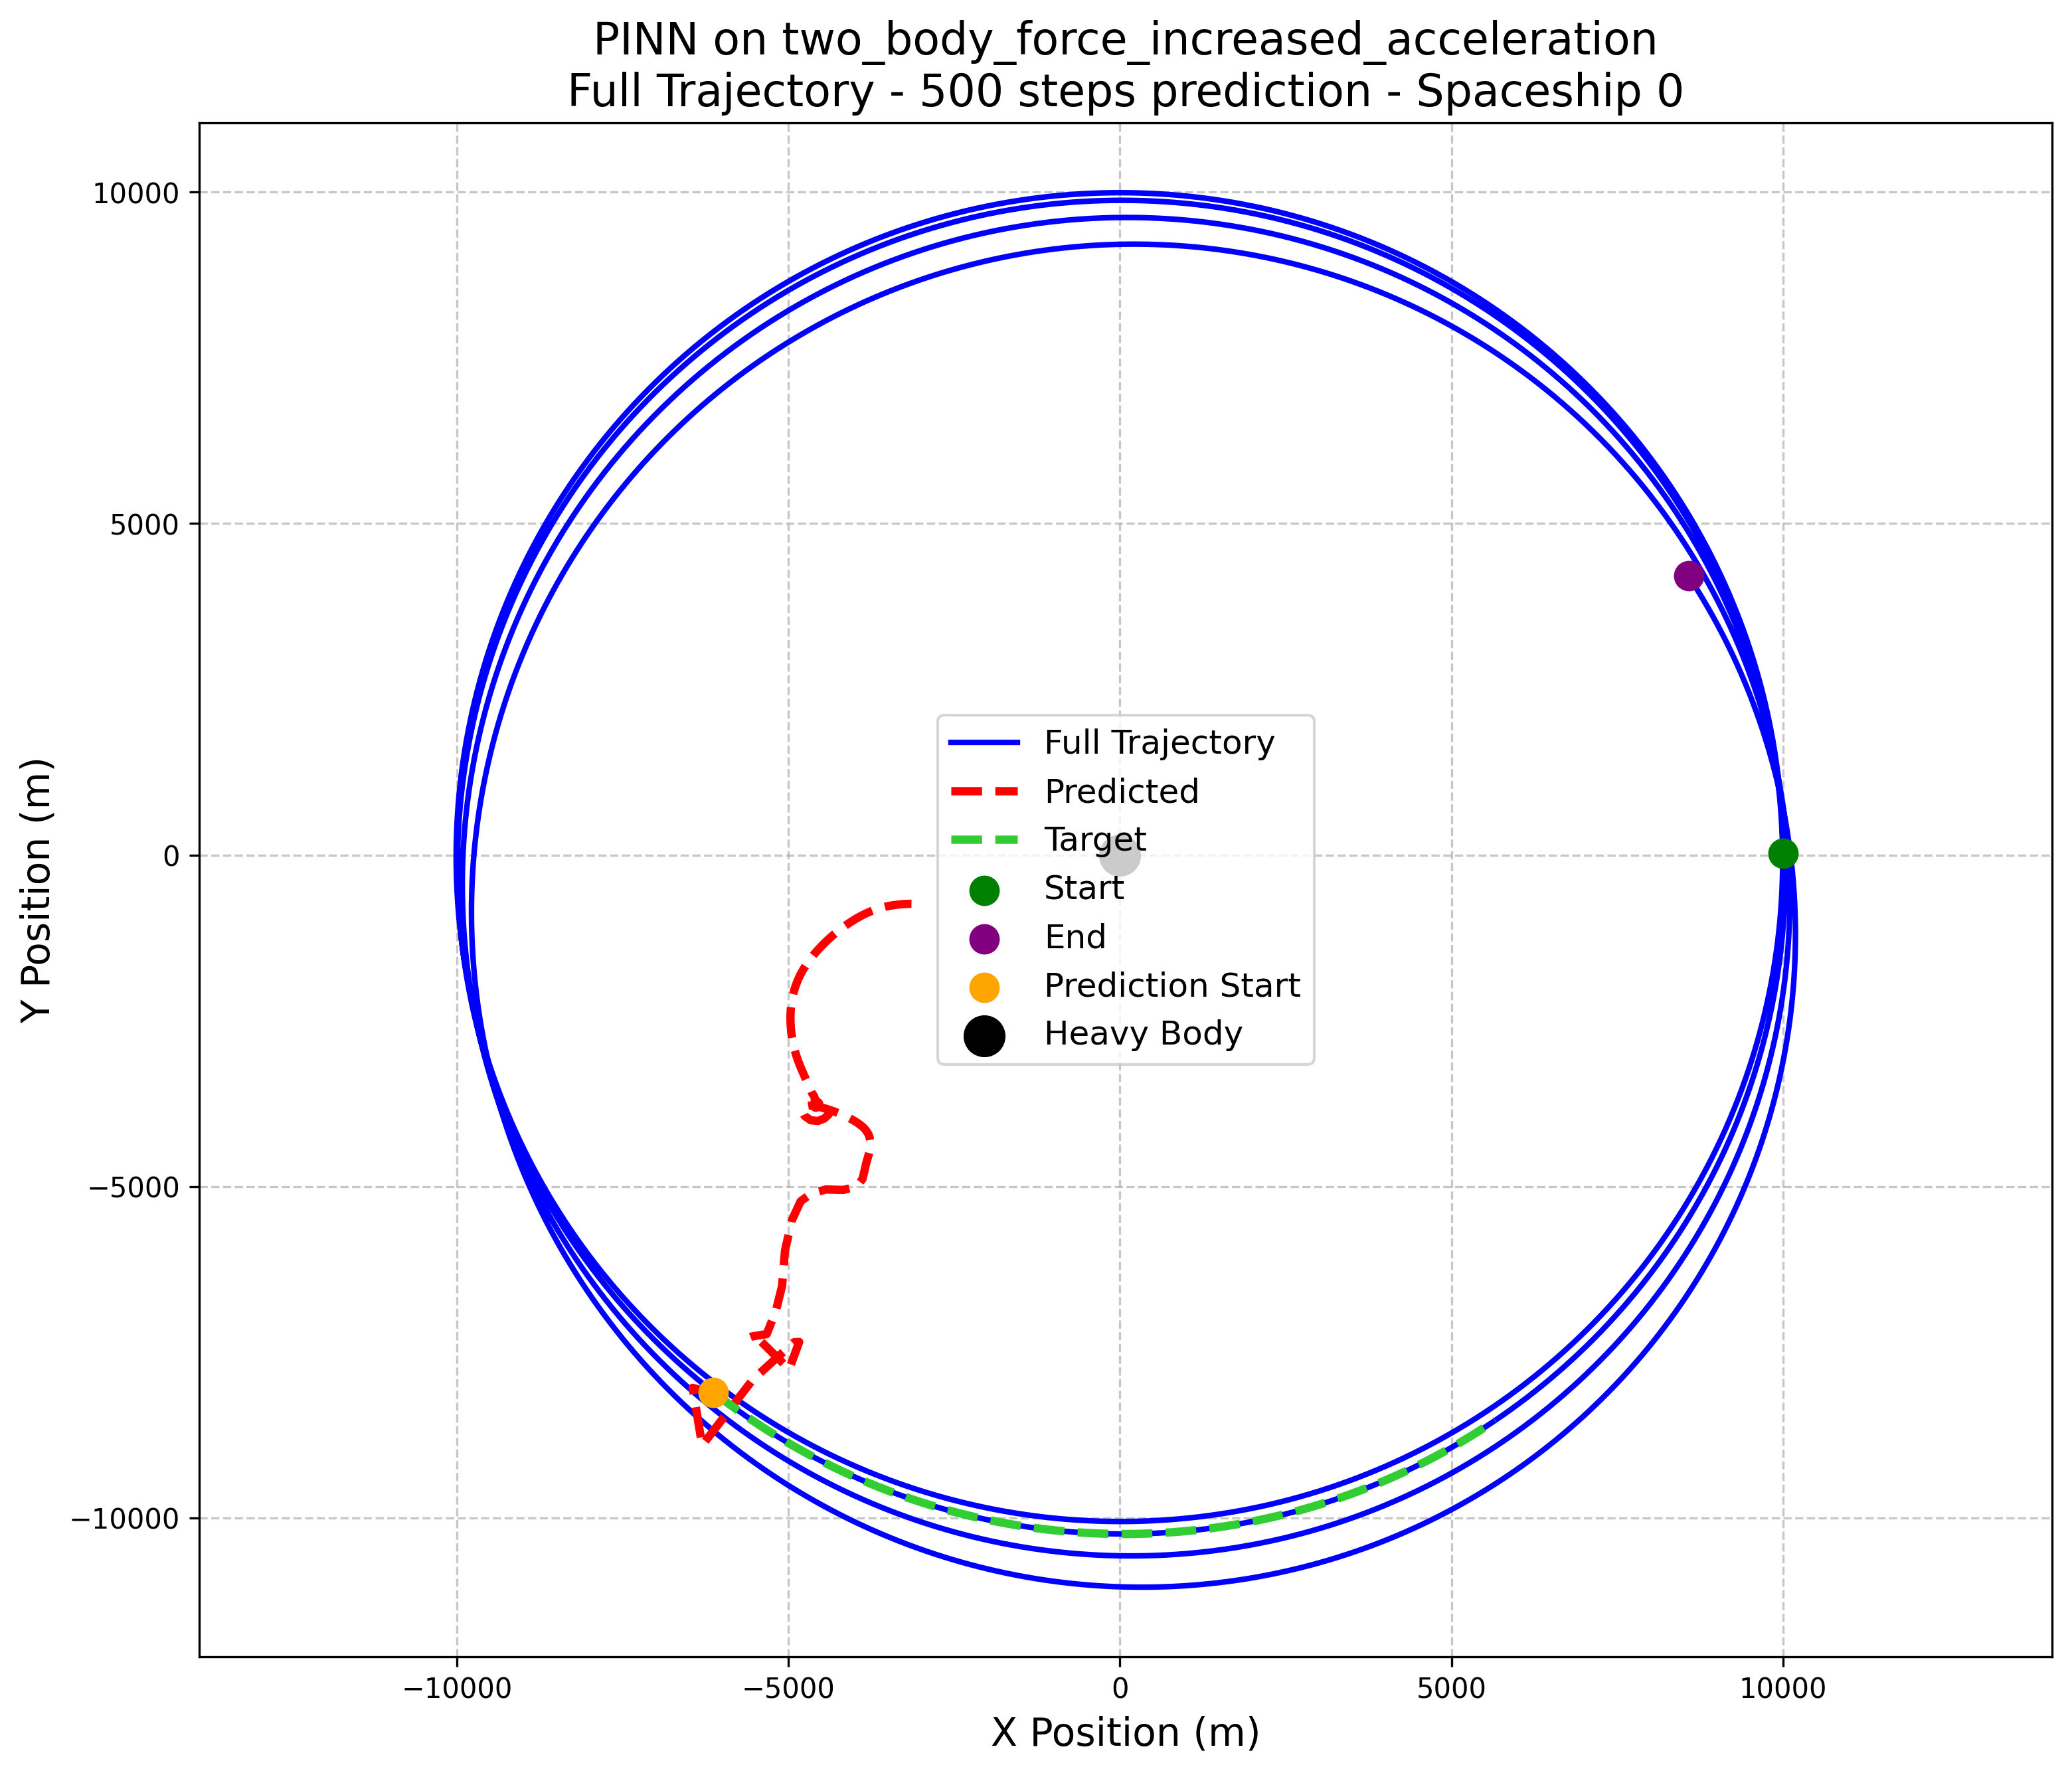
\includegraphics[width=0.27\textwidth]{../inference_results/test/PINN/two_body_force_increased_acceleration/500/full_trajectory_spaceship_0.png}
  \end{tabular}
\end{figure}


\section{Three-Body Problem Trajectory Predictions}
\label{sec:three_body_predictions}
\begin{figure}[H]
  \centering
  \caption{Three-Body Problem: Model Predictions vs. Actual Trajectories for first spaceship}
  \label{fig:three_body_predictions}
  \begin{tabular}{cccc}
      & Train & Validation & Test \\
      MLP &
      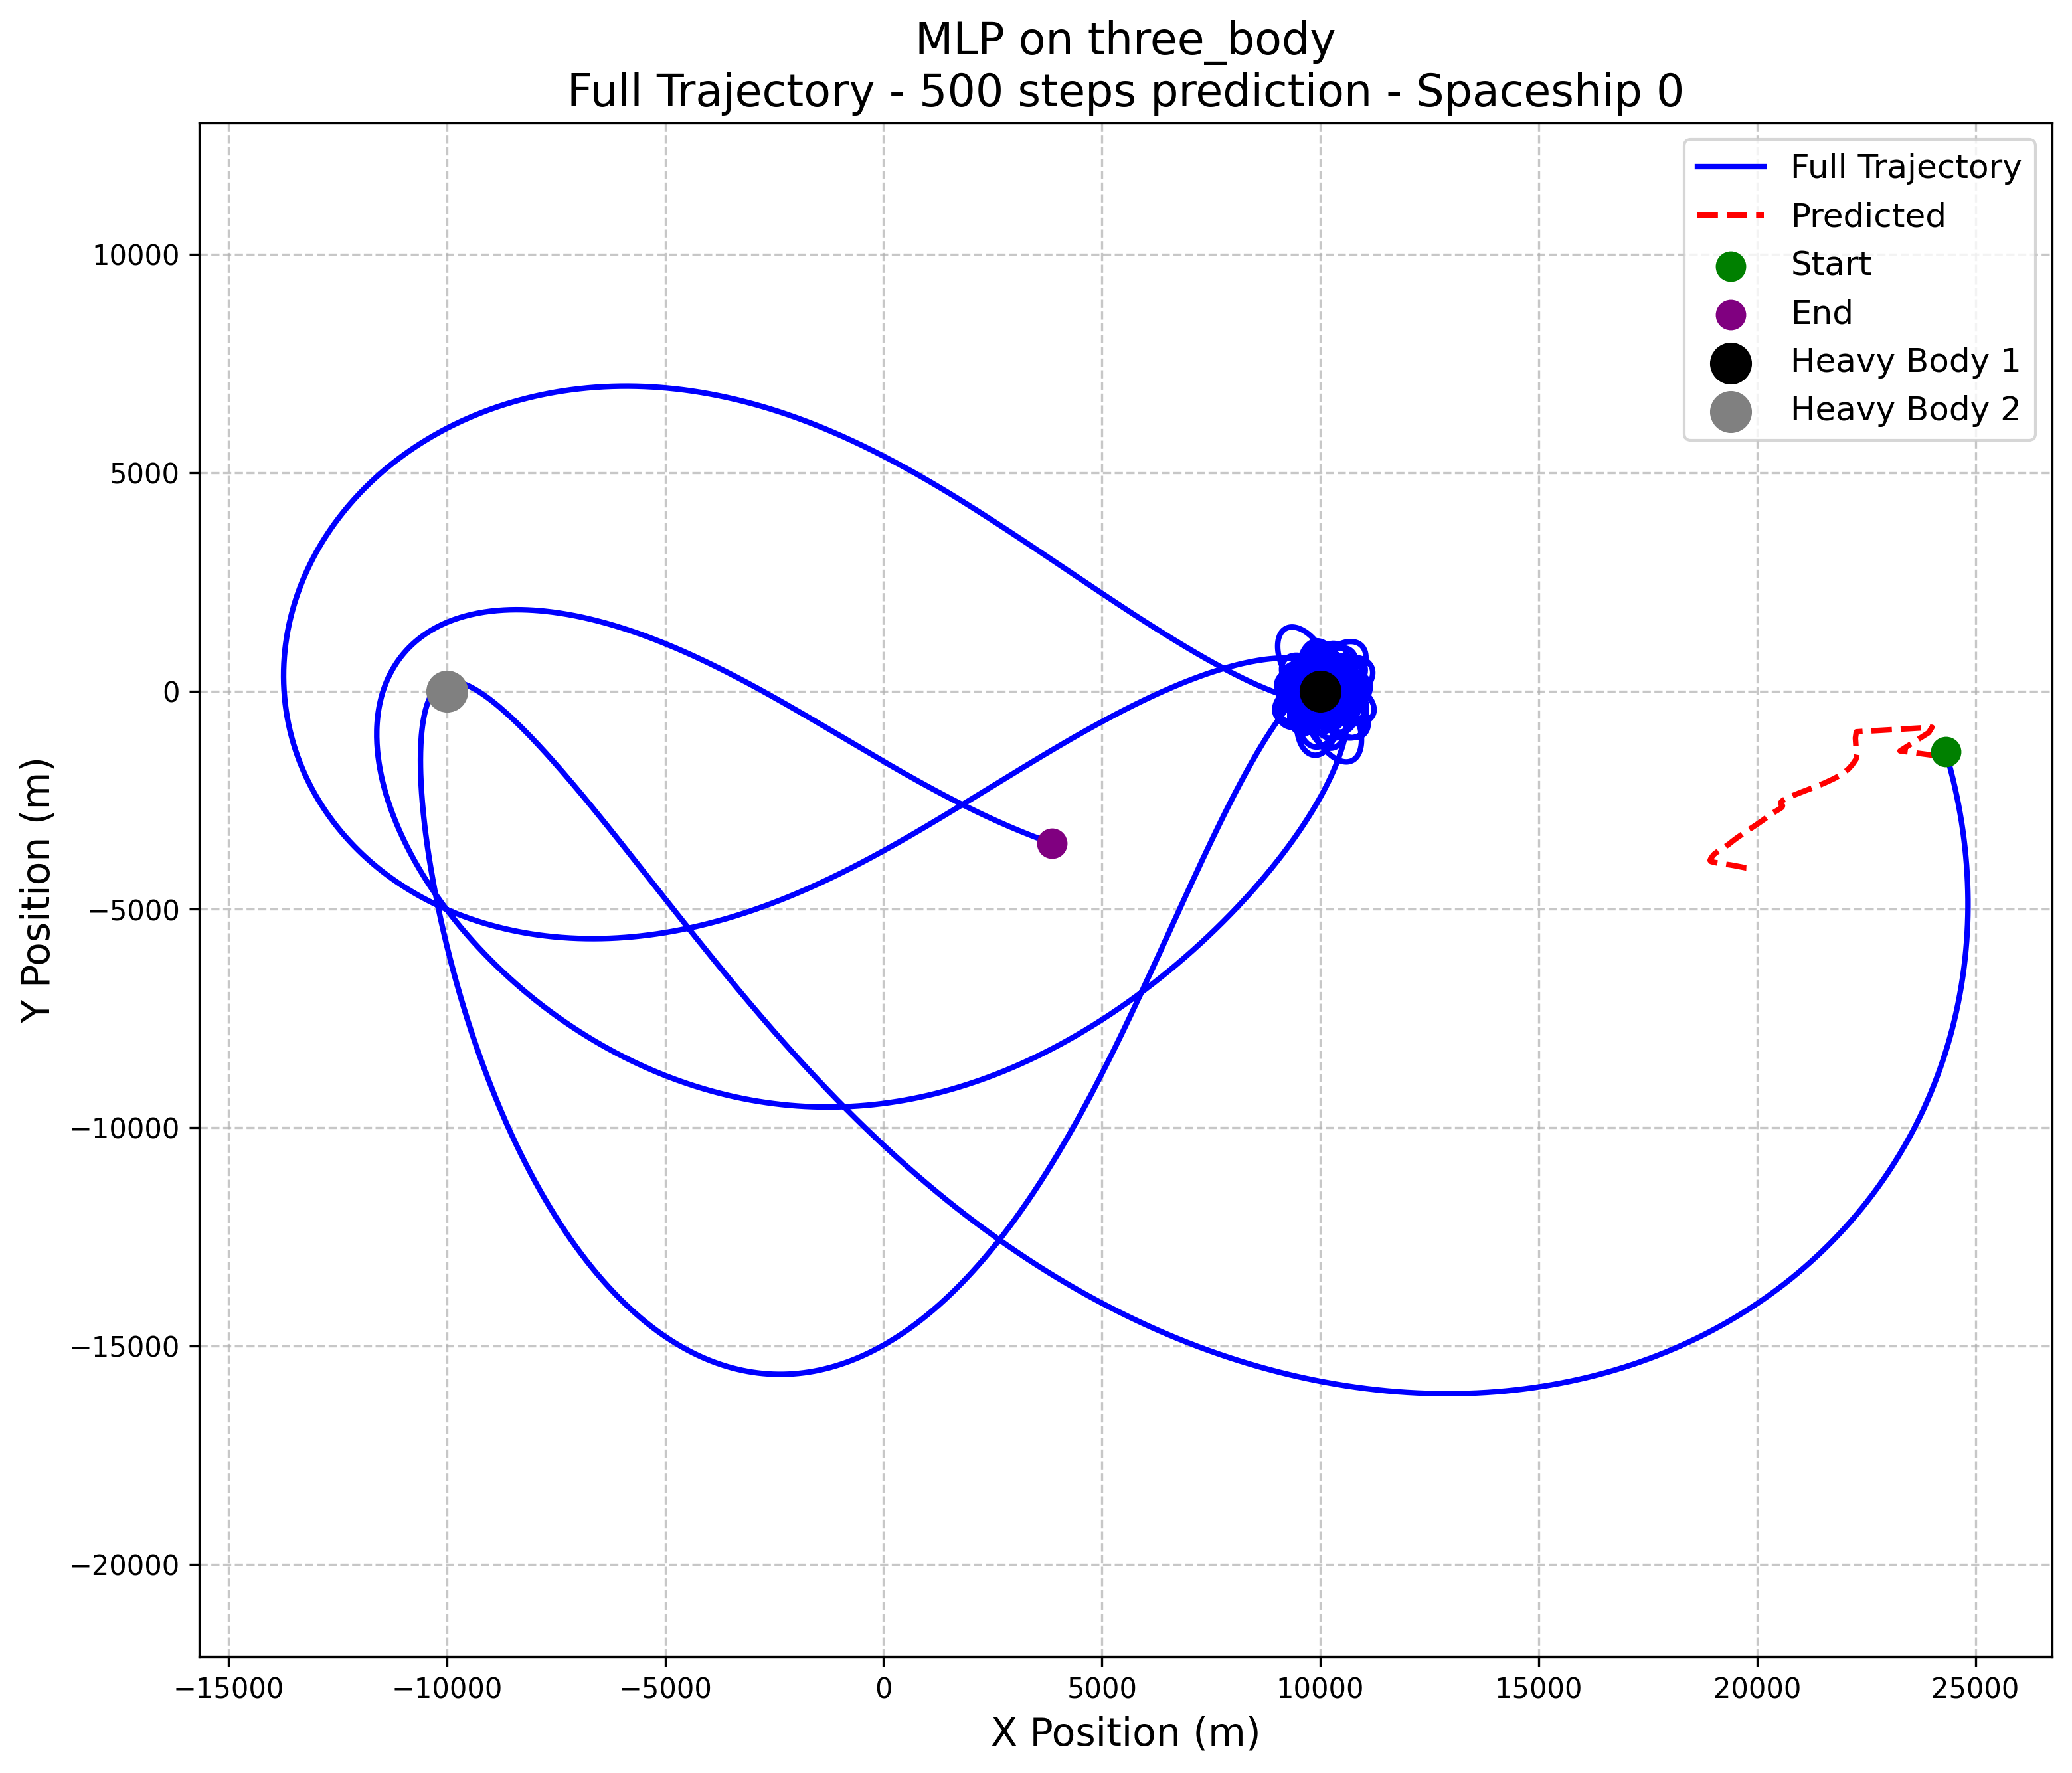
\includegraphics[width=0.27\textwidth]{../inference_results/train/MLP/three_body/500/full_trajectory_spaceship_0.png} &
      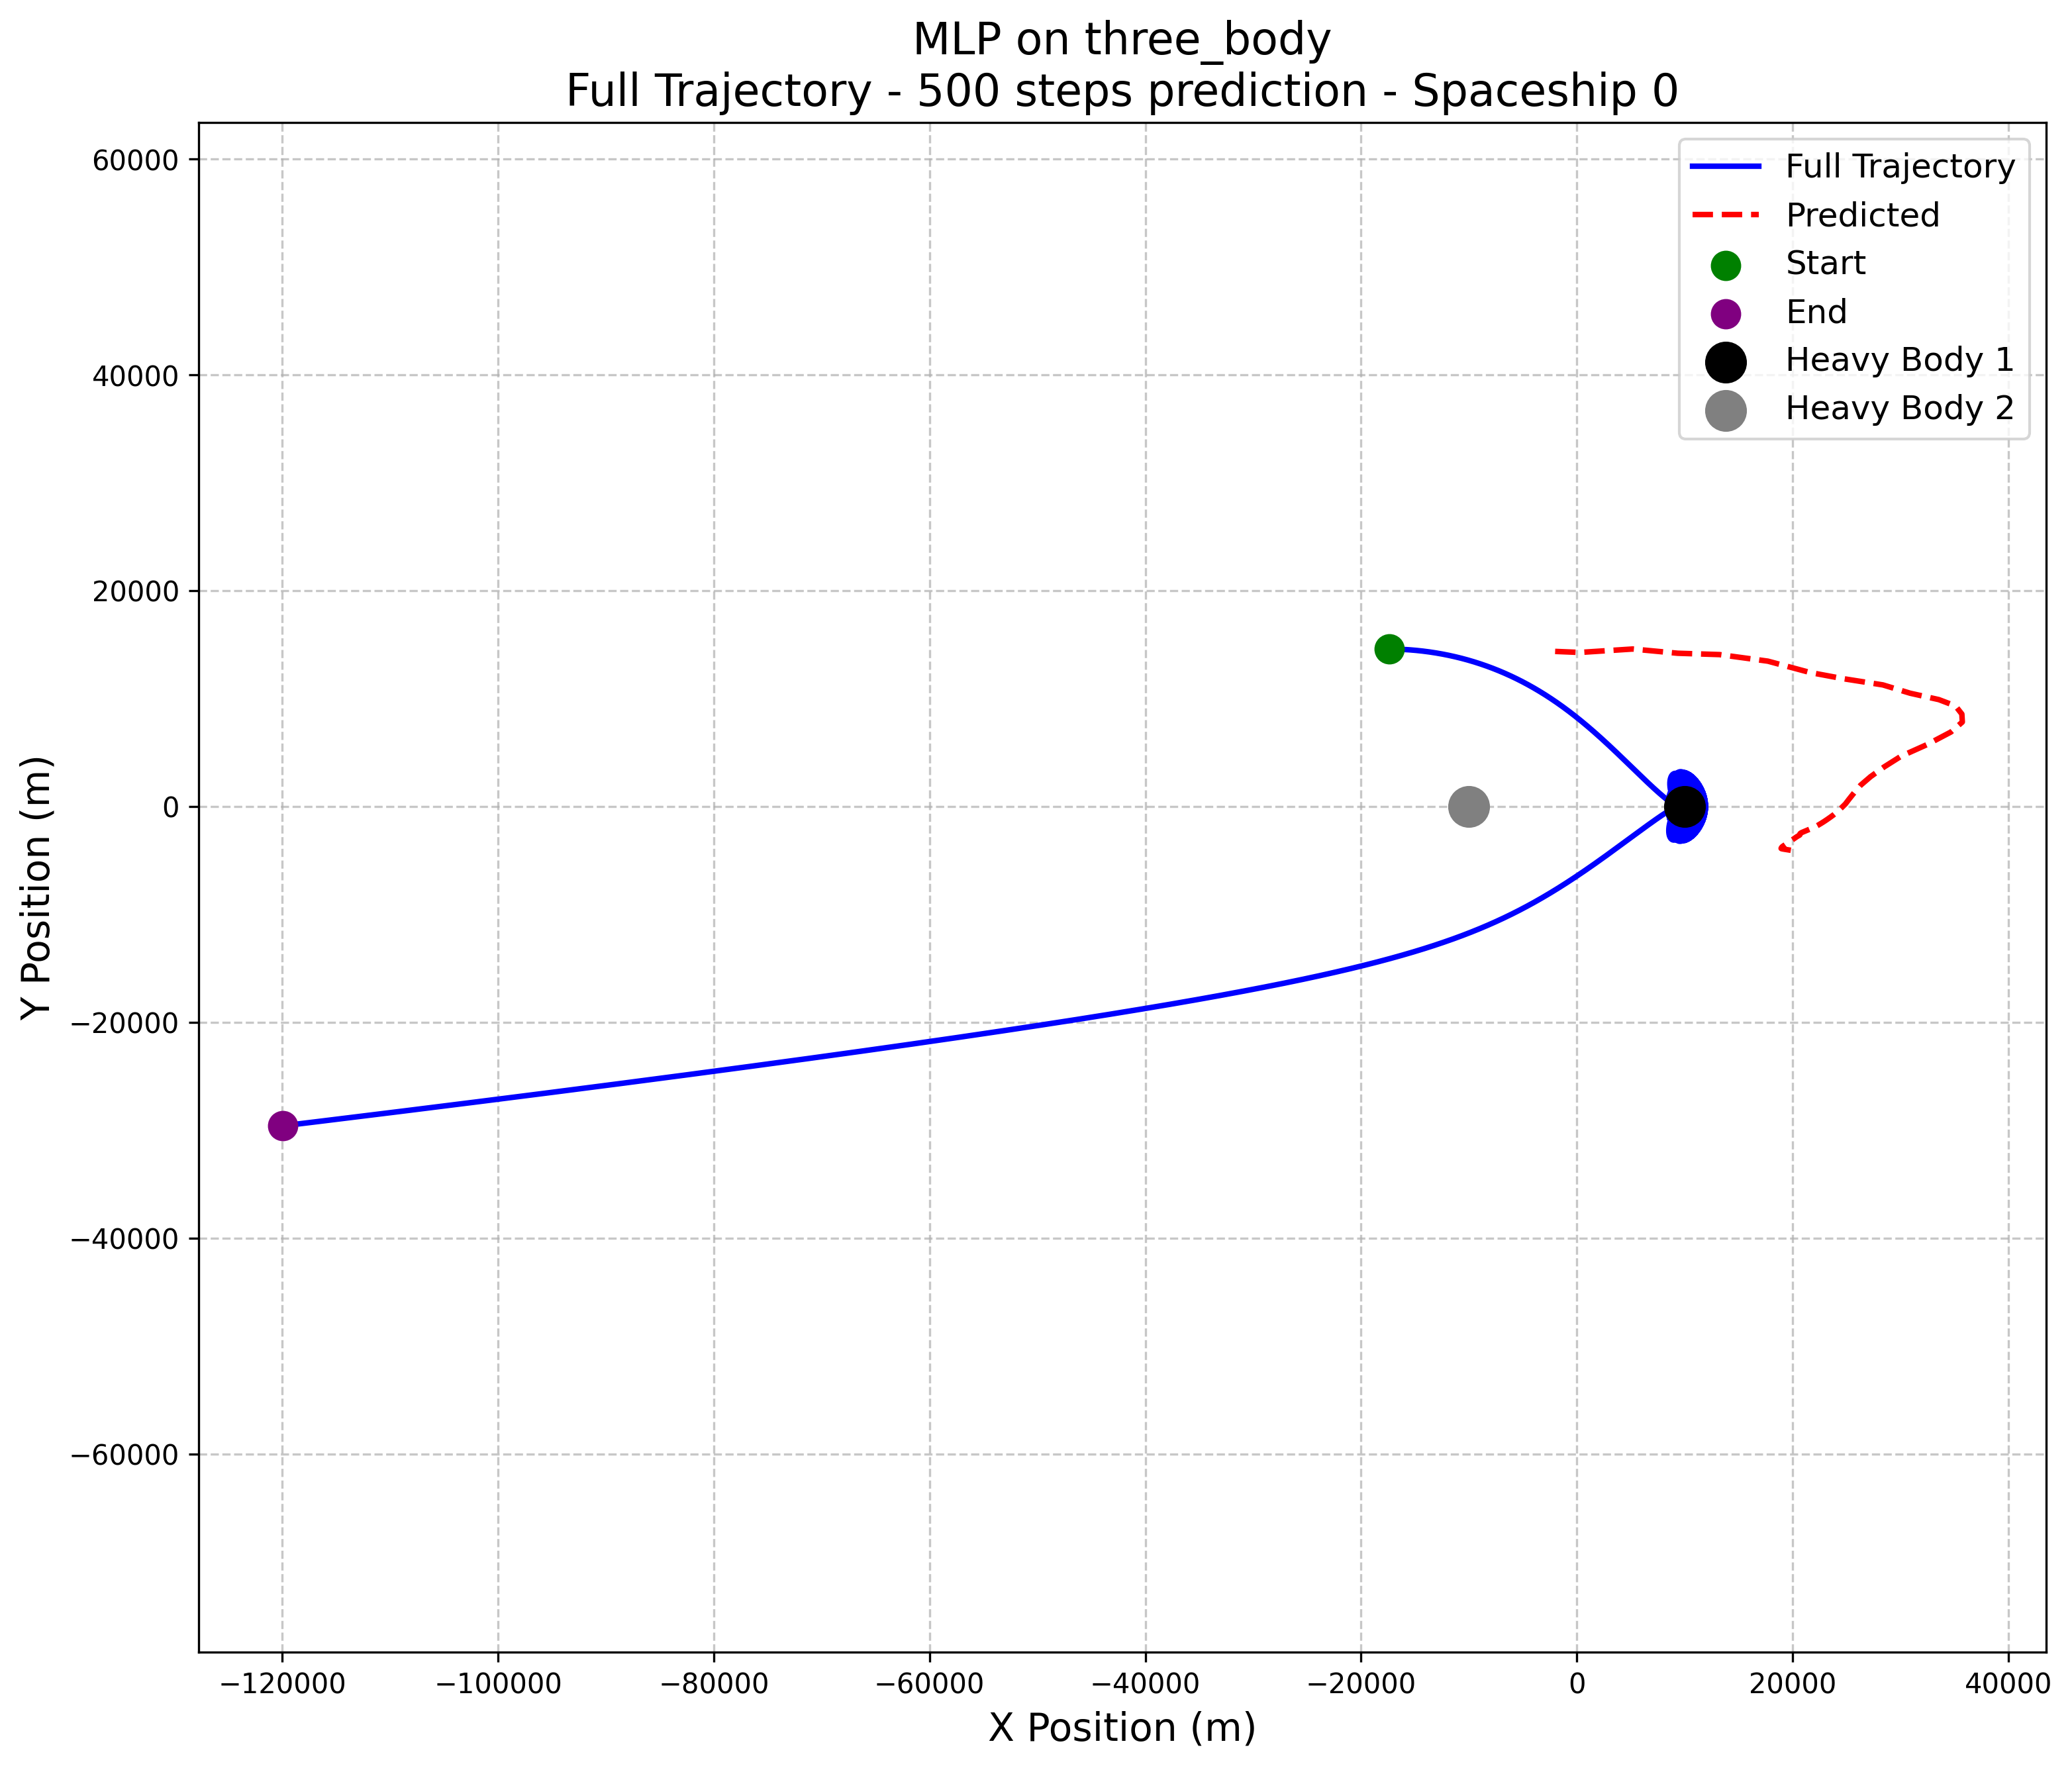
\includegraphics[width=0.27\textwidth]{../inference_results/val/MLP/three_body/500/full_trajectory_spaceship_0.png} &
      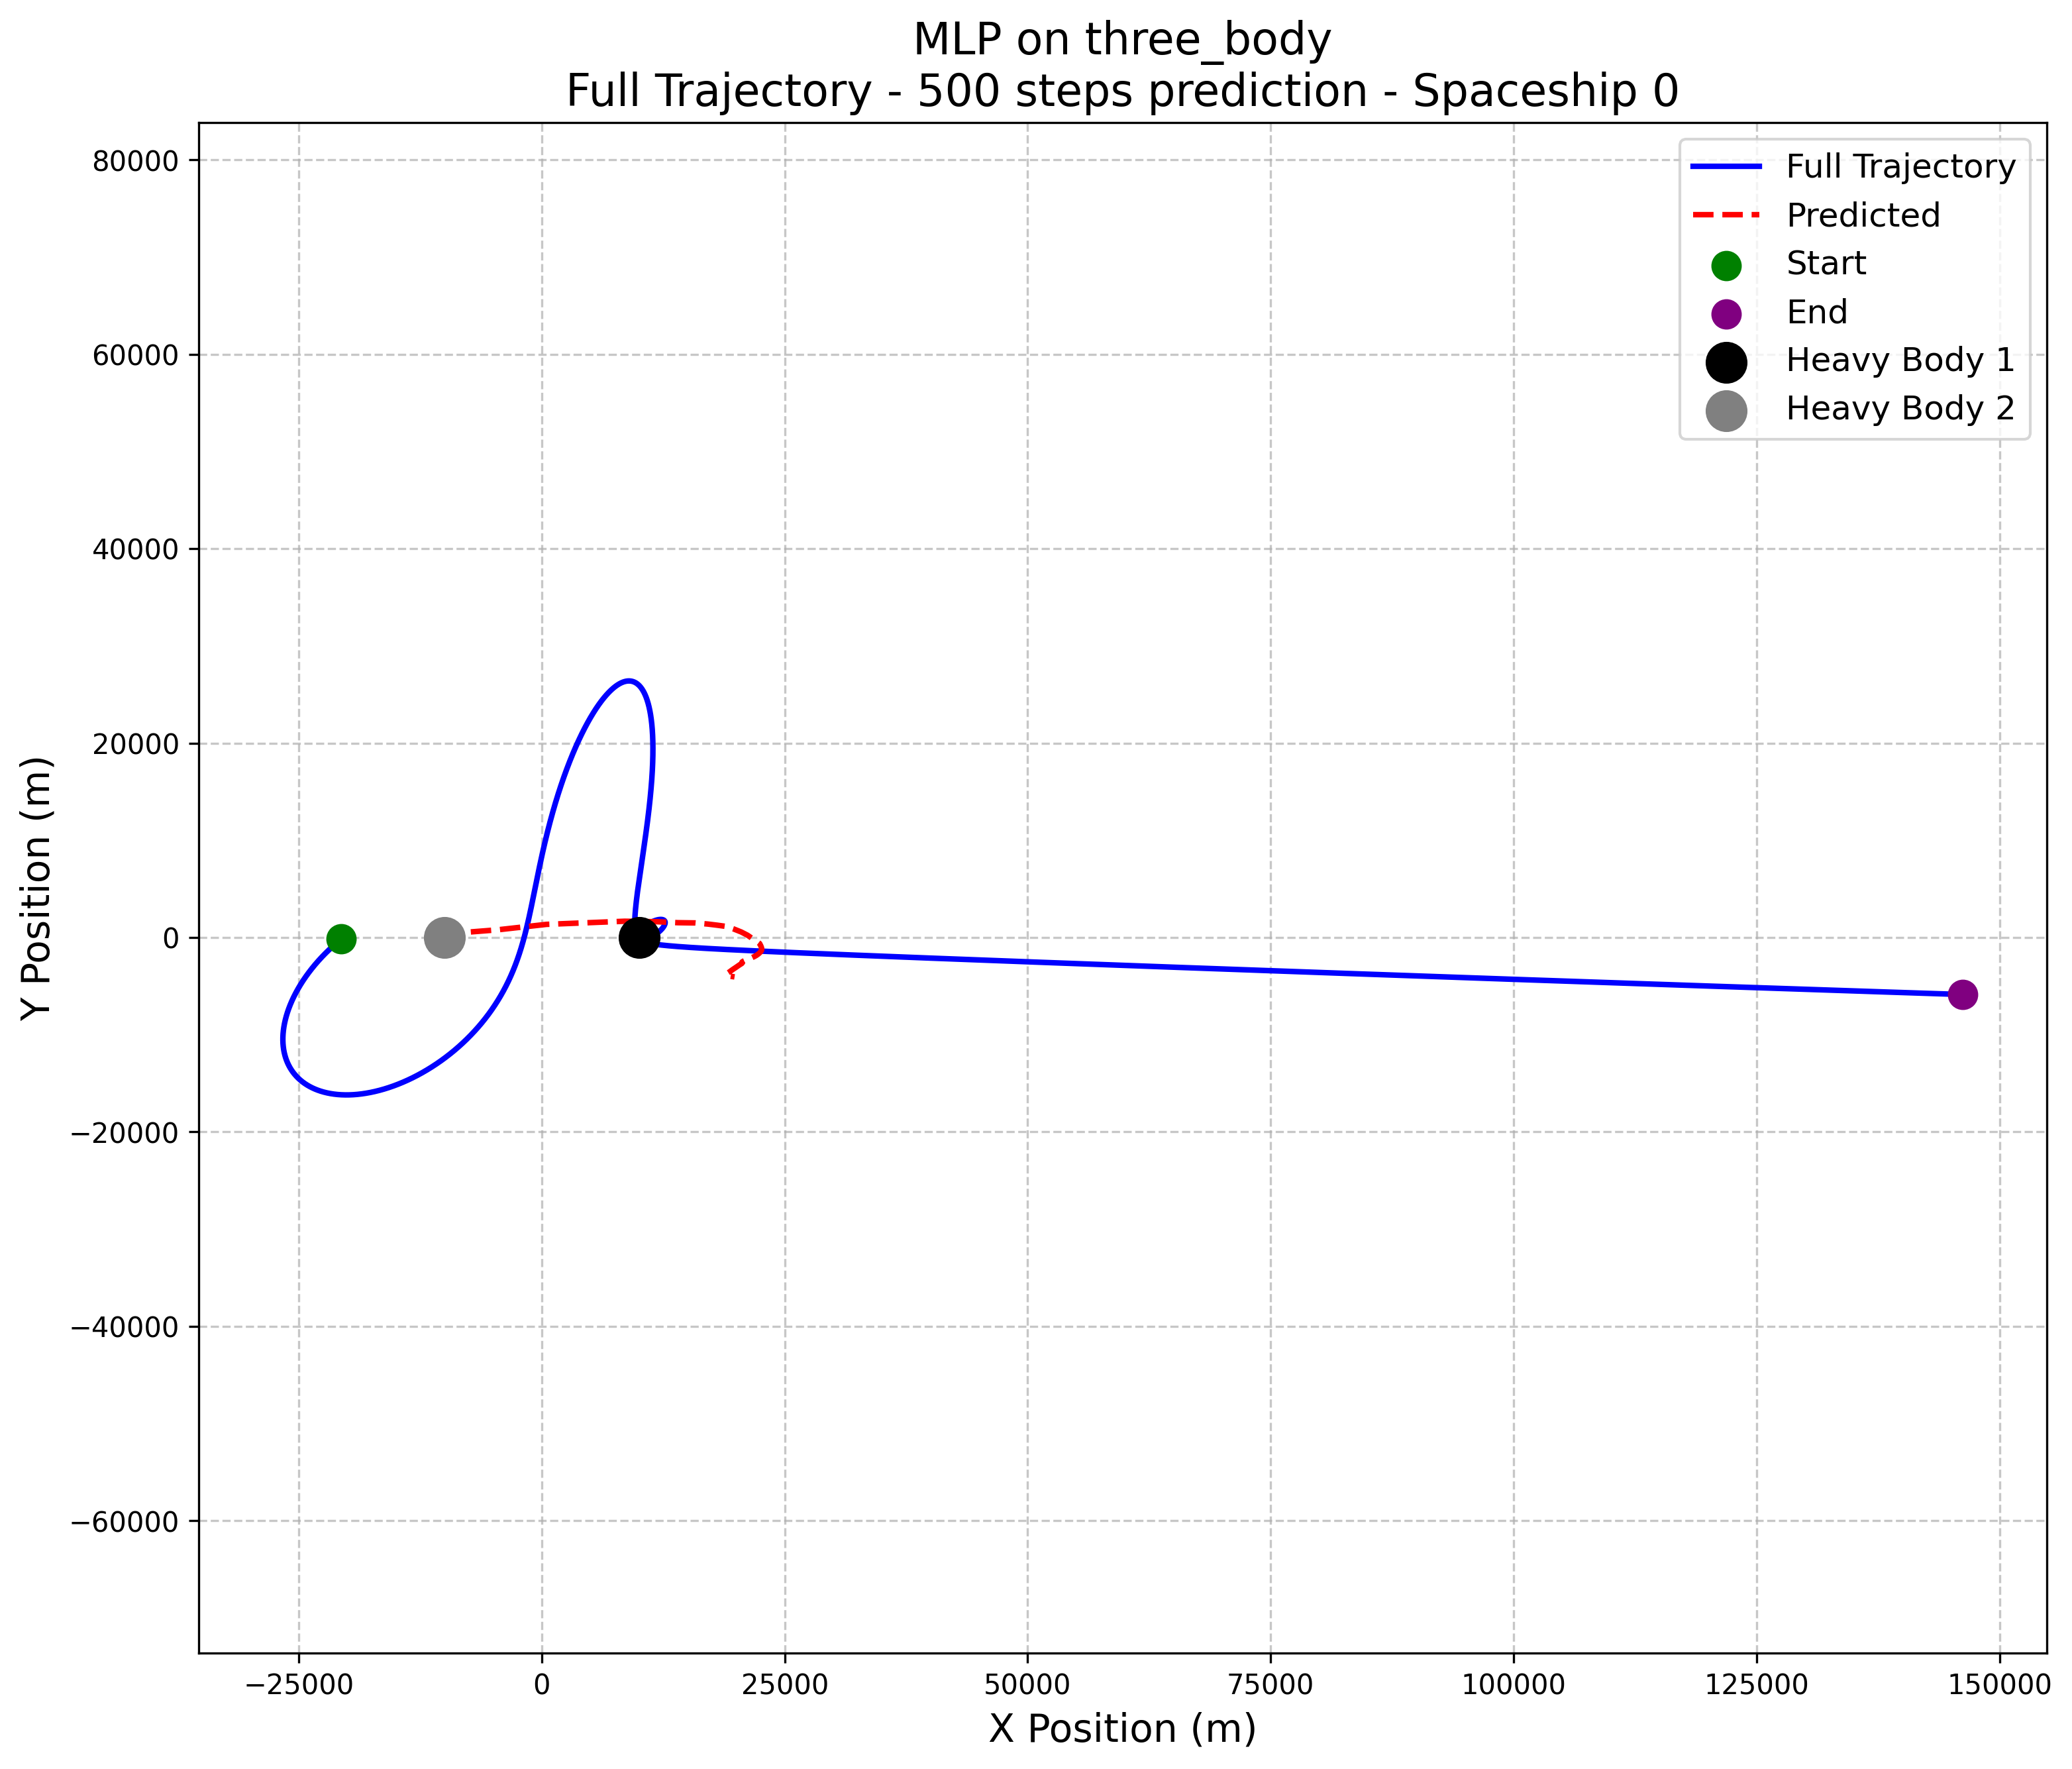
\includegraphics[width=0.27\textwidth]{../inference_results/test/MLP/three_body/500/full_trajectory_spaceship_0.png} \\
      LSTM &
      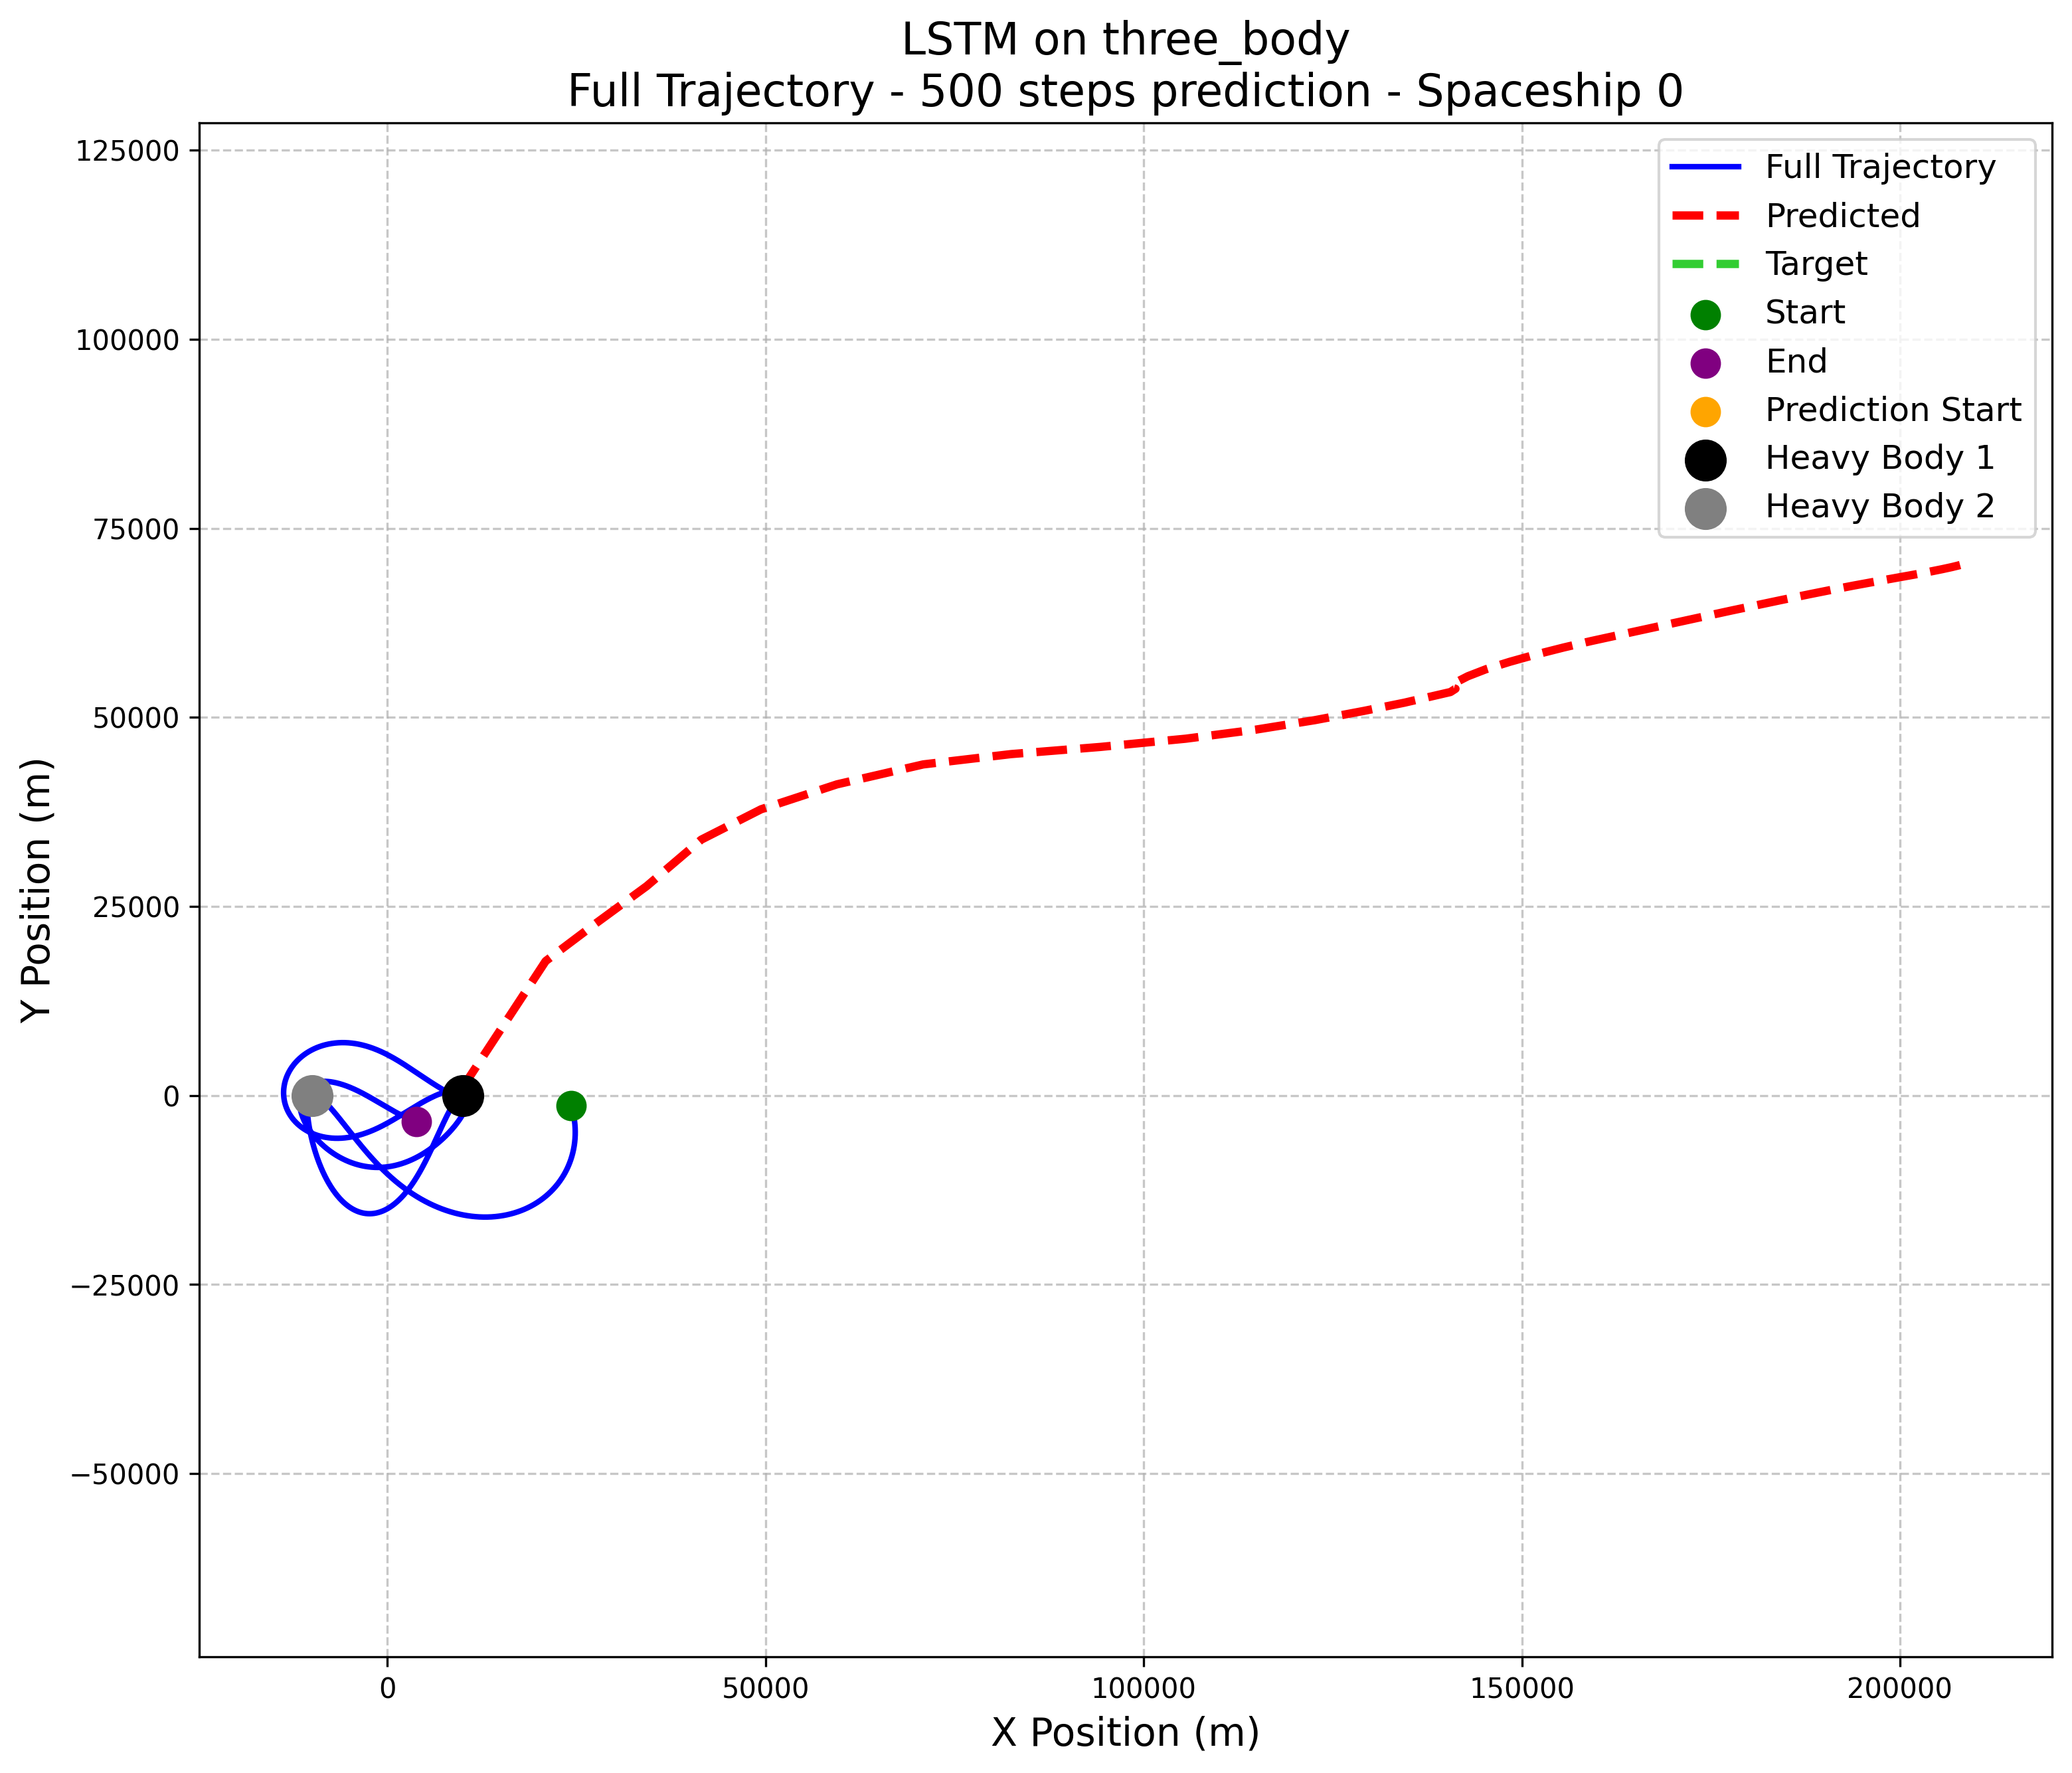
\includegraphics[width=0.27\textwidth]{../inference_results/train/LSTM/three_body/500/full_trajectory_spaceship_0.png} &
      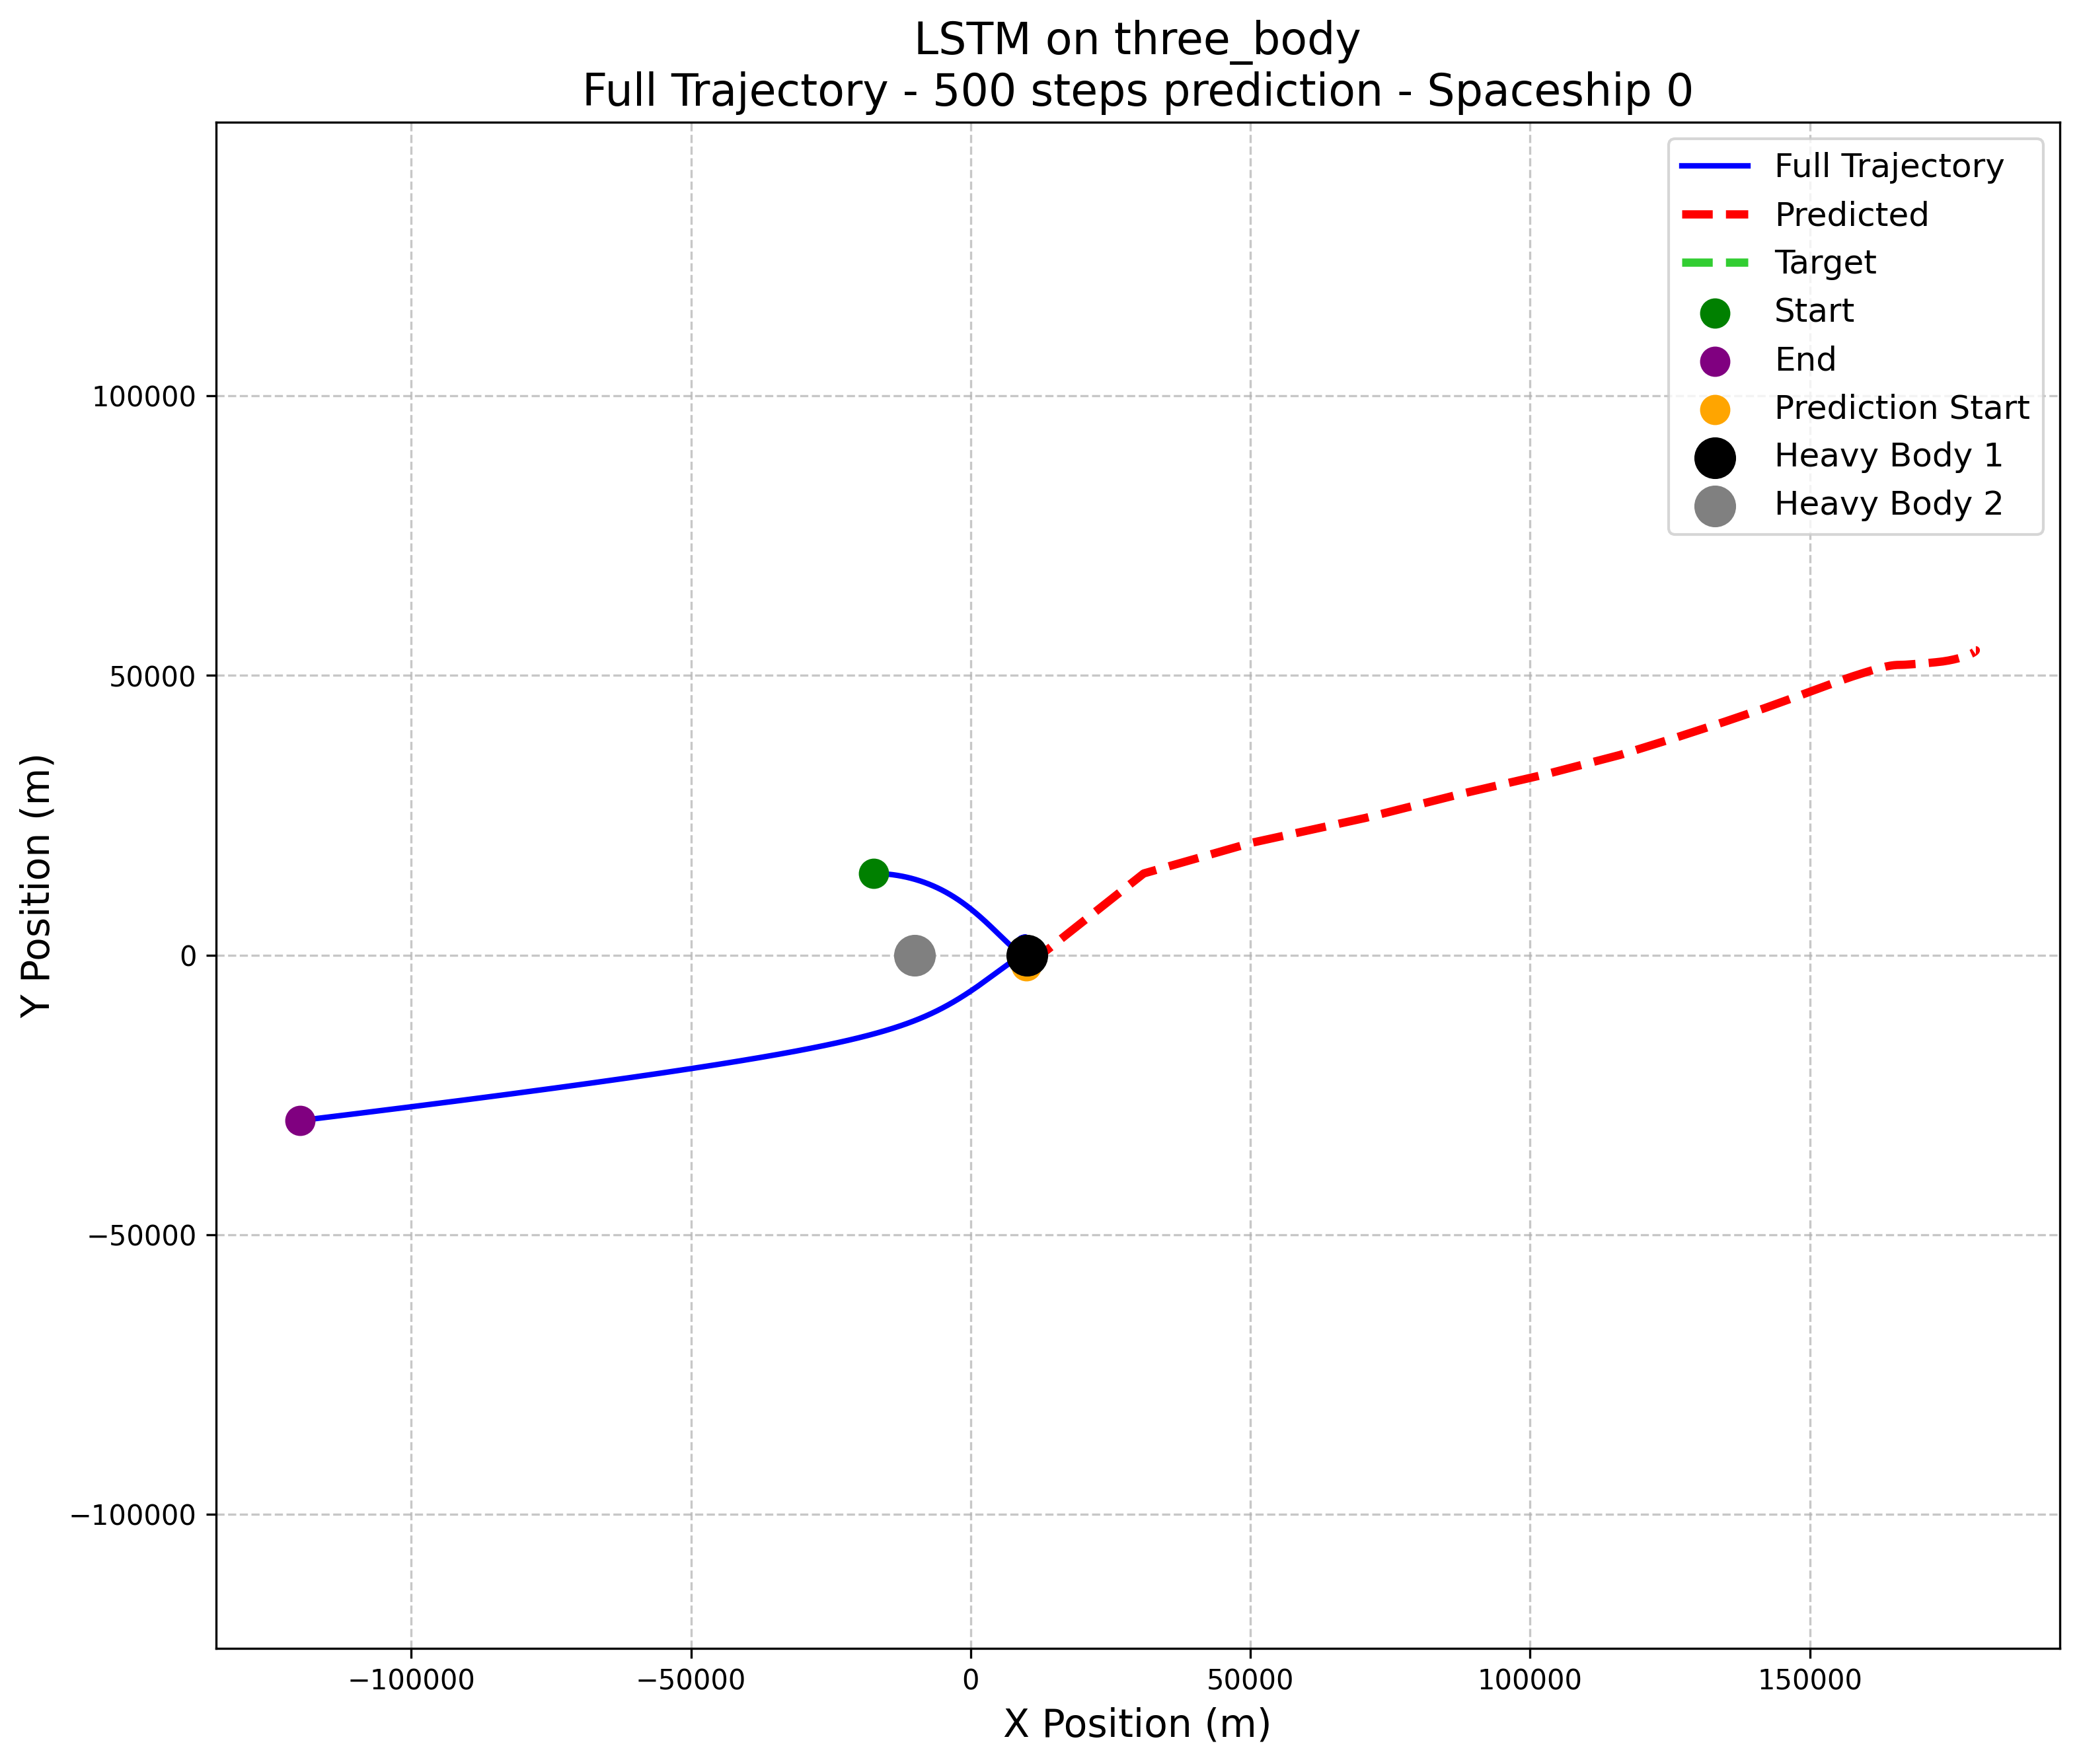
\includegraphics[width=0.27\textwidth]{../inference_results/val/LSTM/three_body/500/full_trajectory_spaceship_0.png} &
      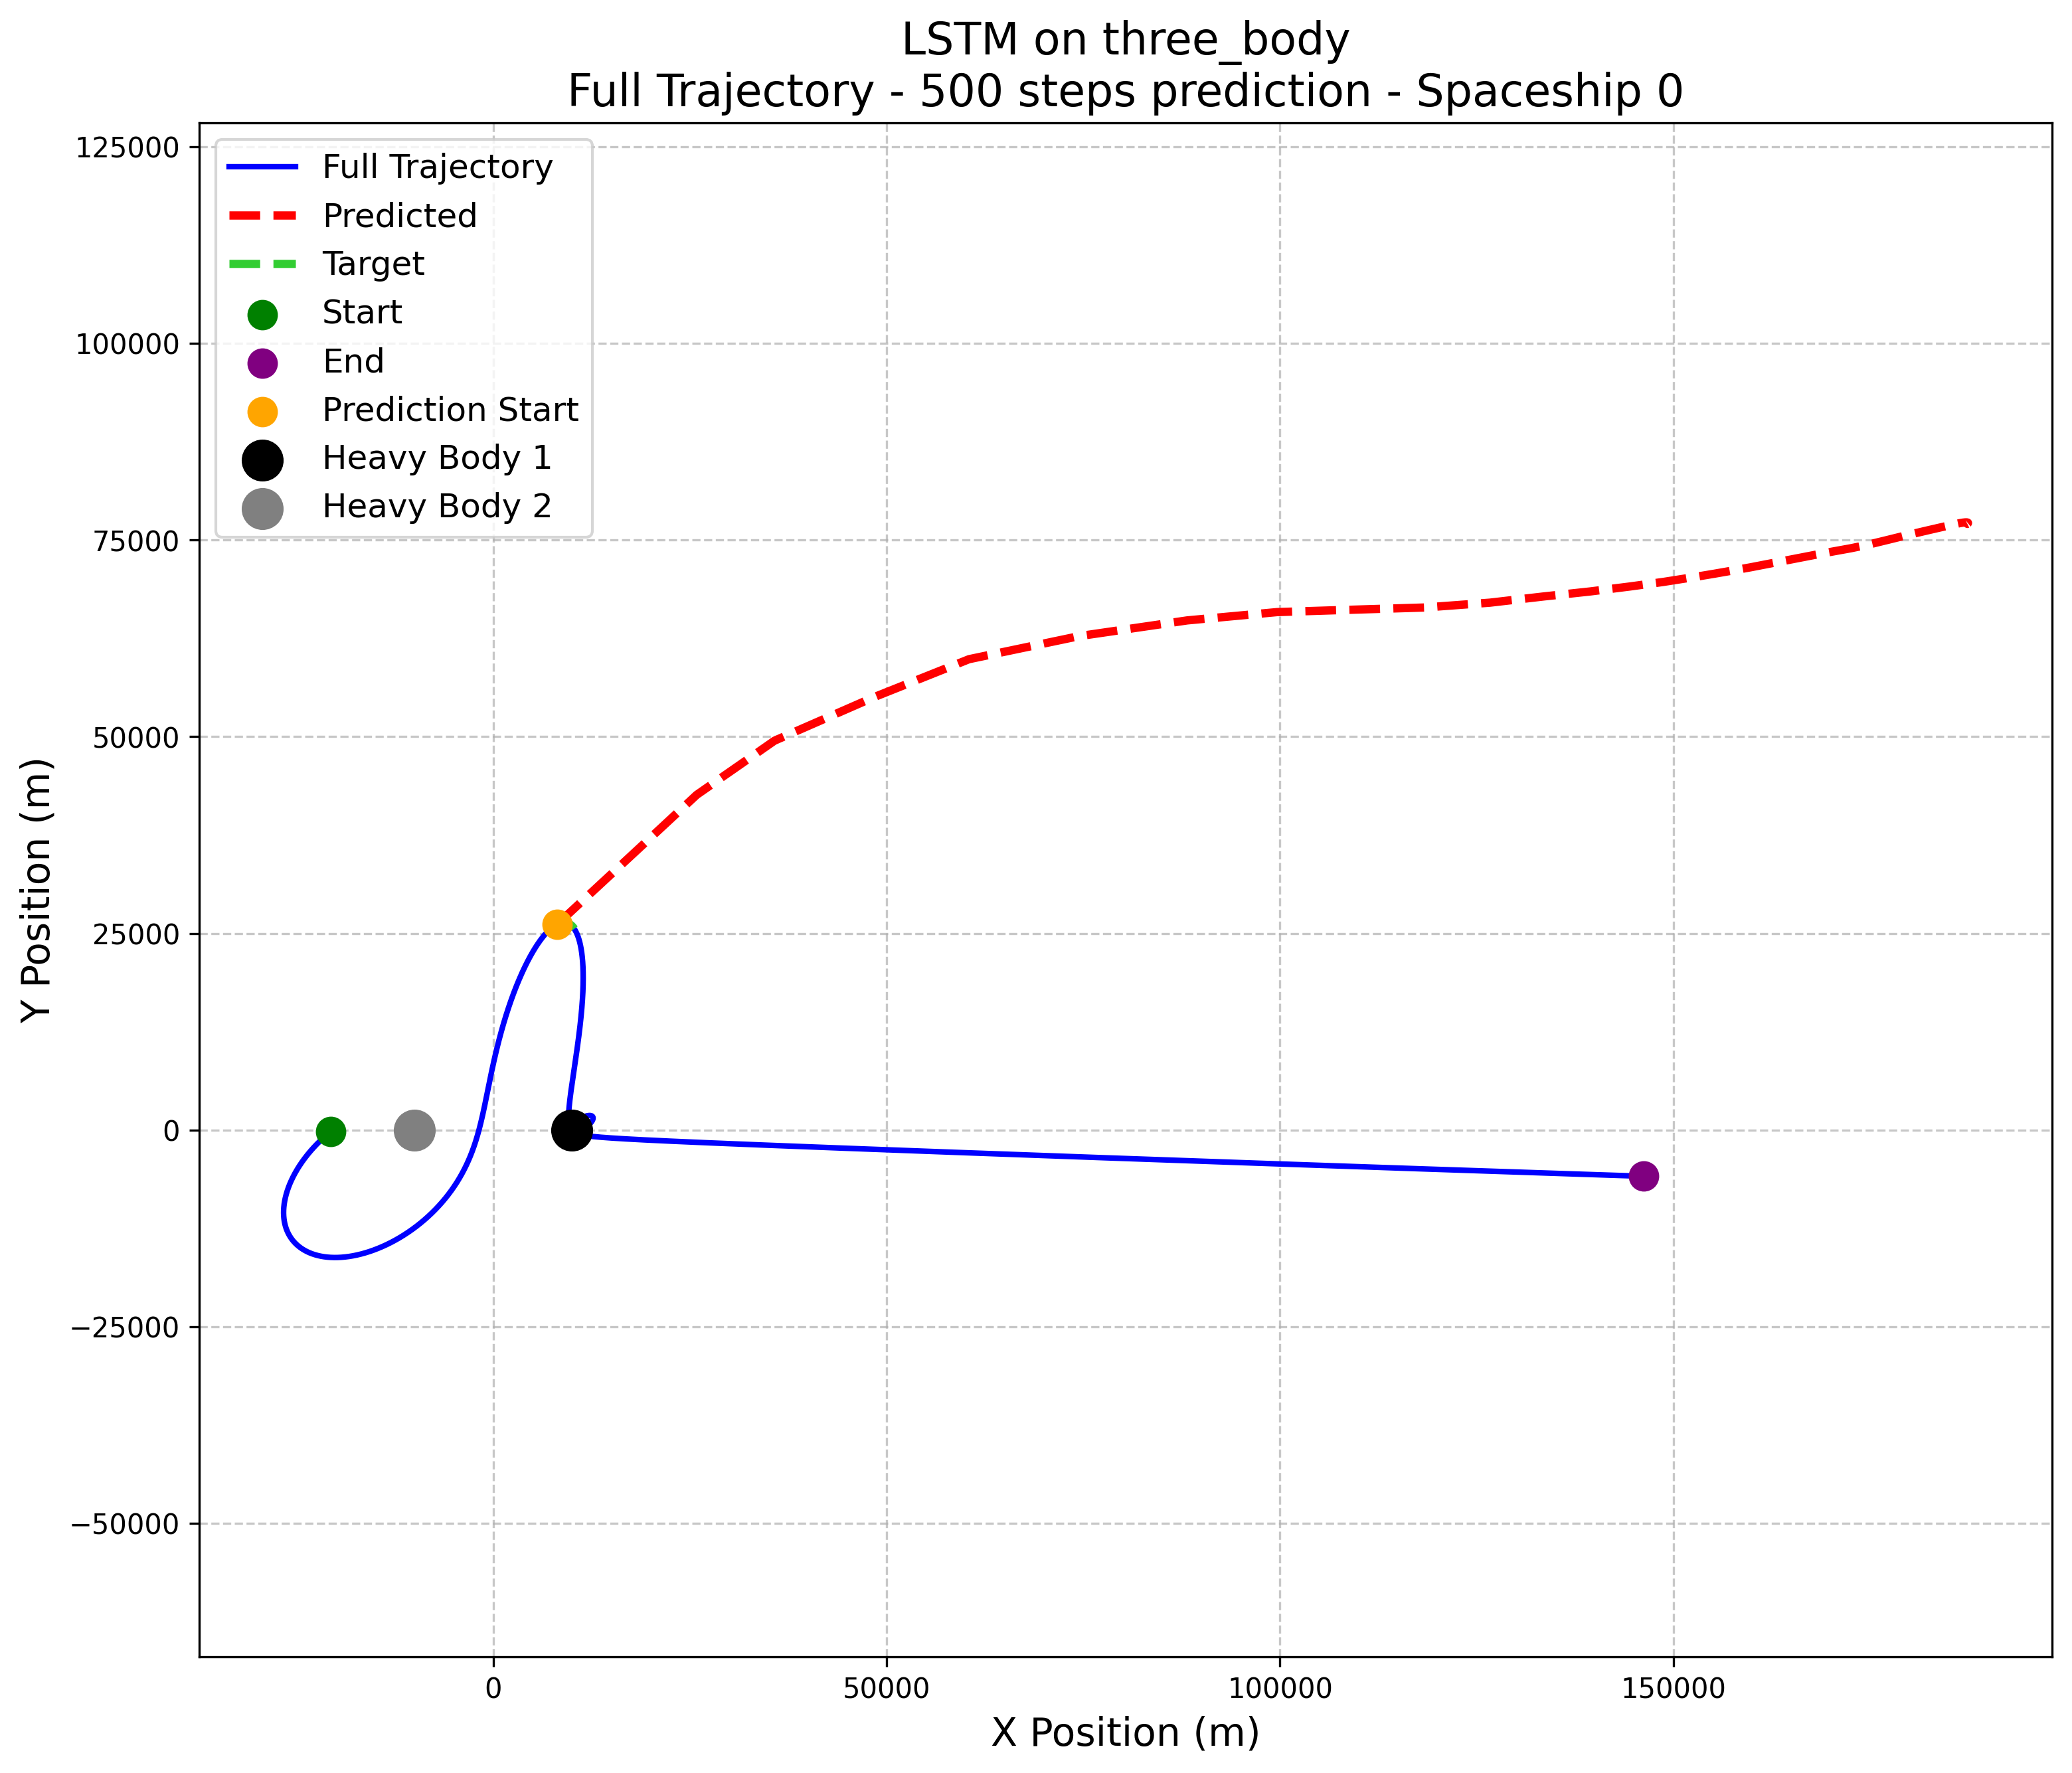
\includegraphics[width=0.27\textwidth]{../inference_results/test/LSTM/three_body/500/full_trajectory_spaceship_0.png} \\
      PINN &
      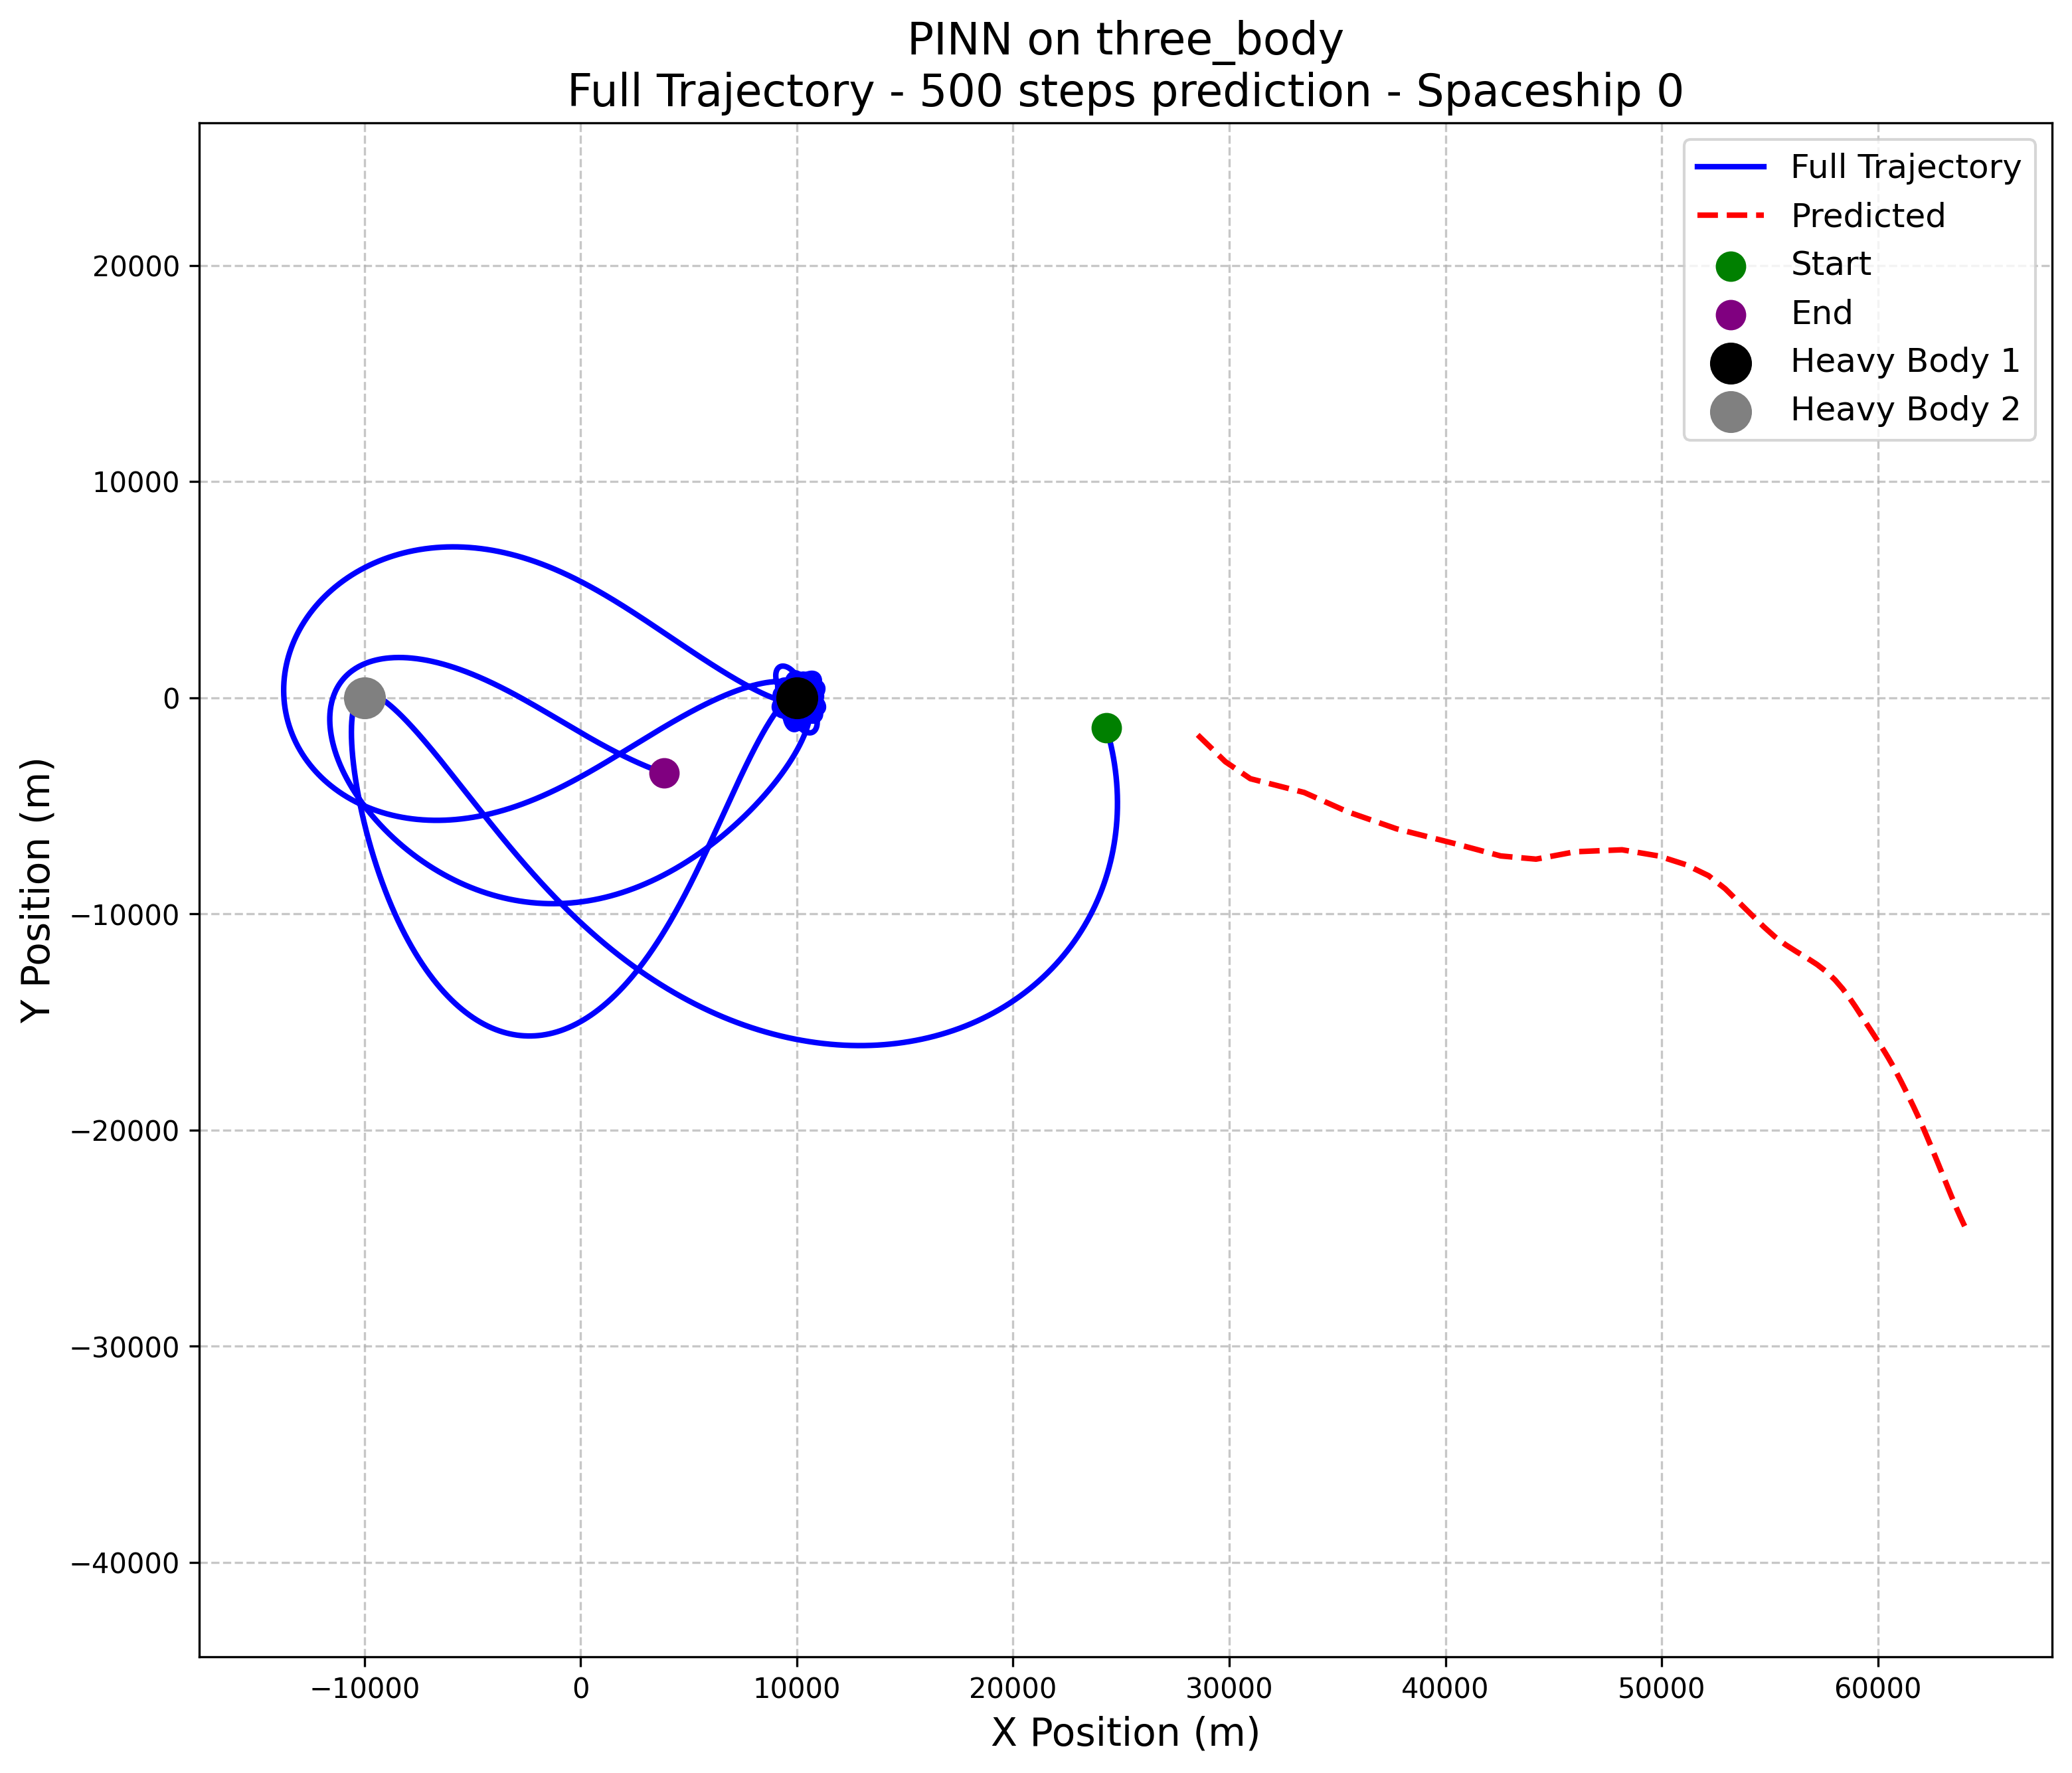
\includegraphics[width=0.27\textwidth]{../inference_results/train/PINN/three_body/500/full_trajectory_spaceship_0.png} &
      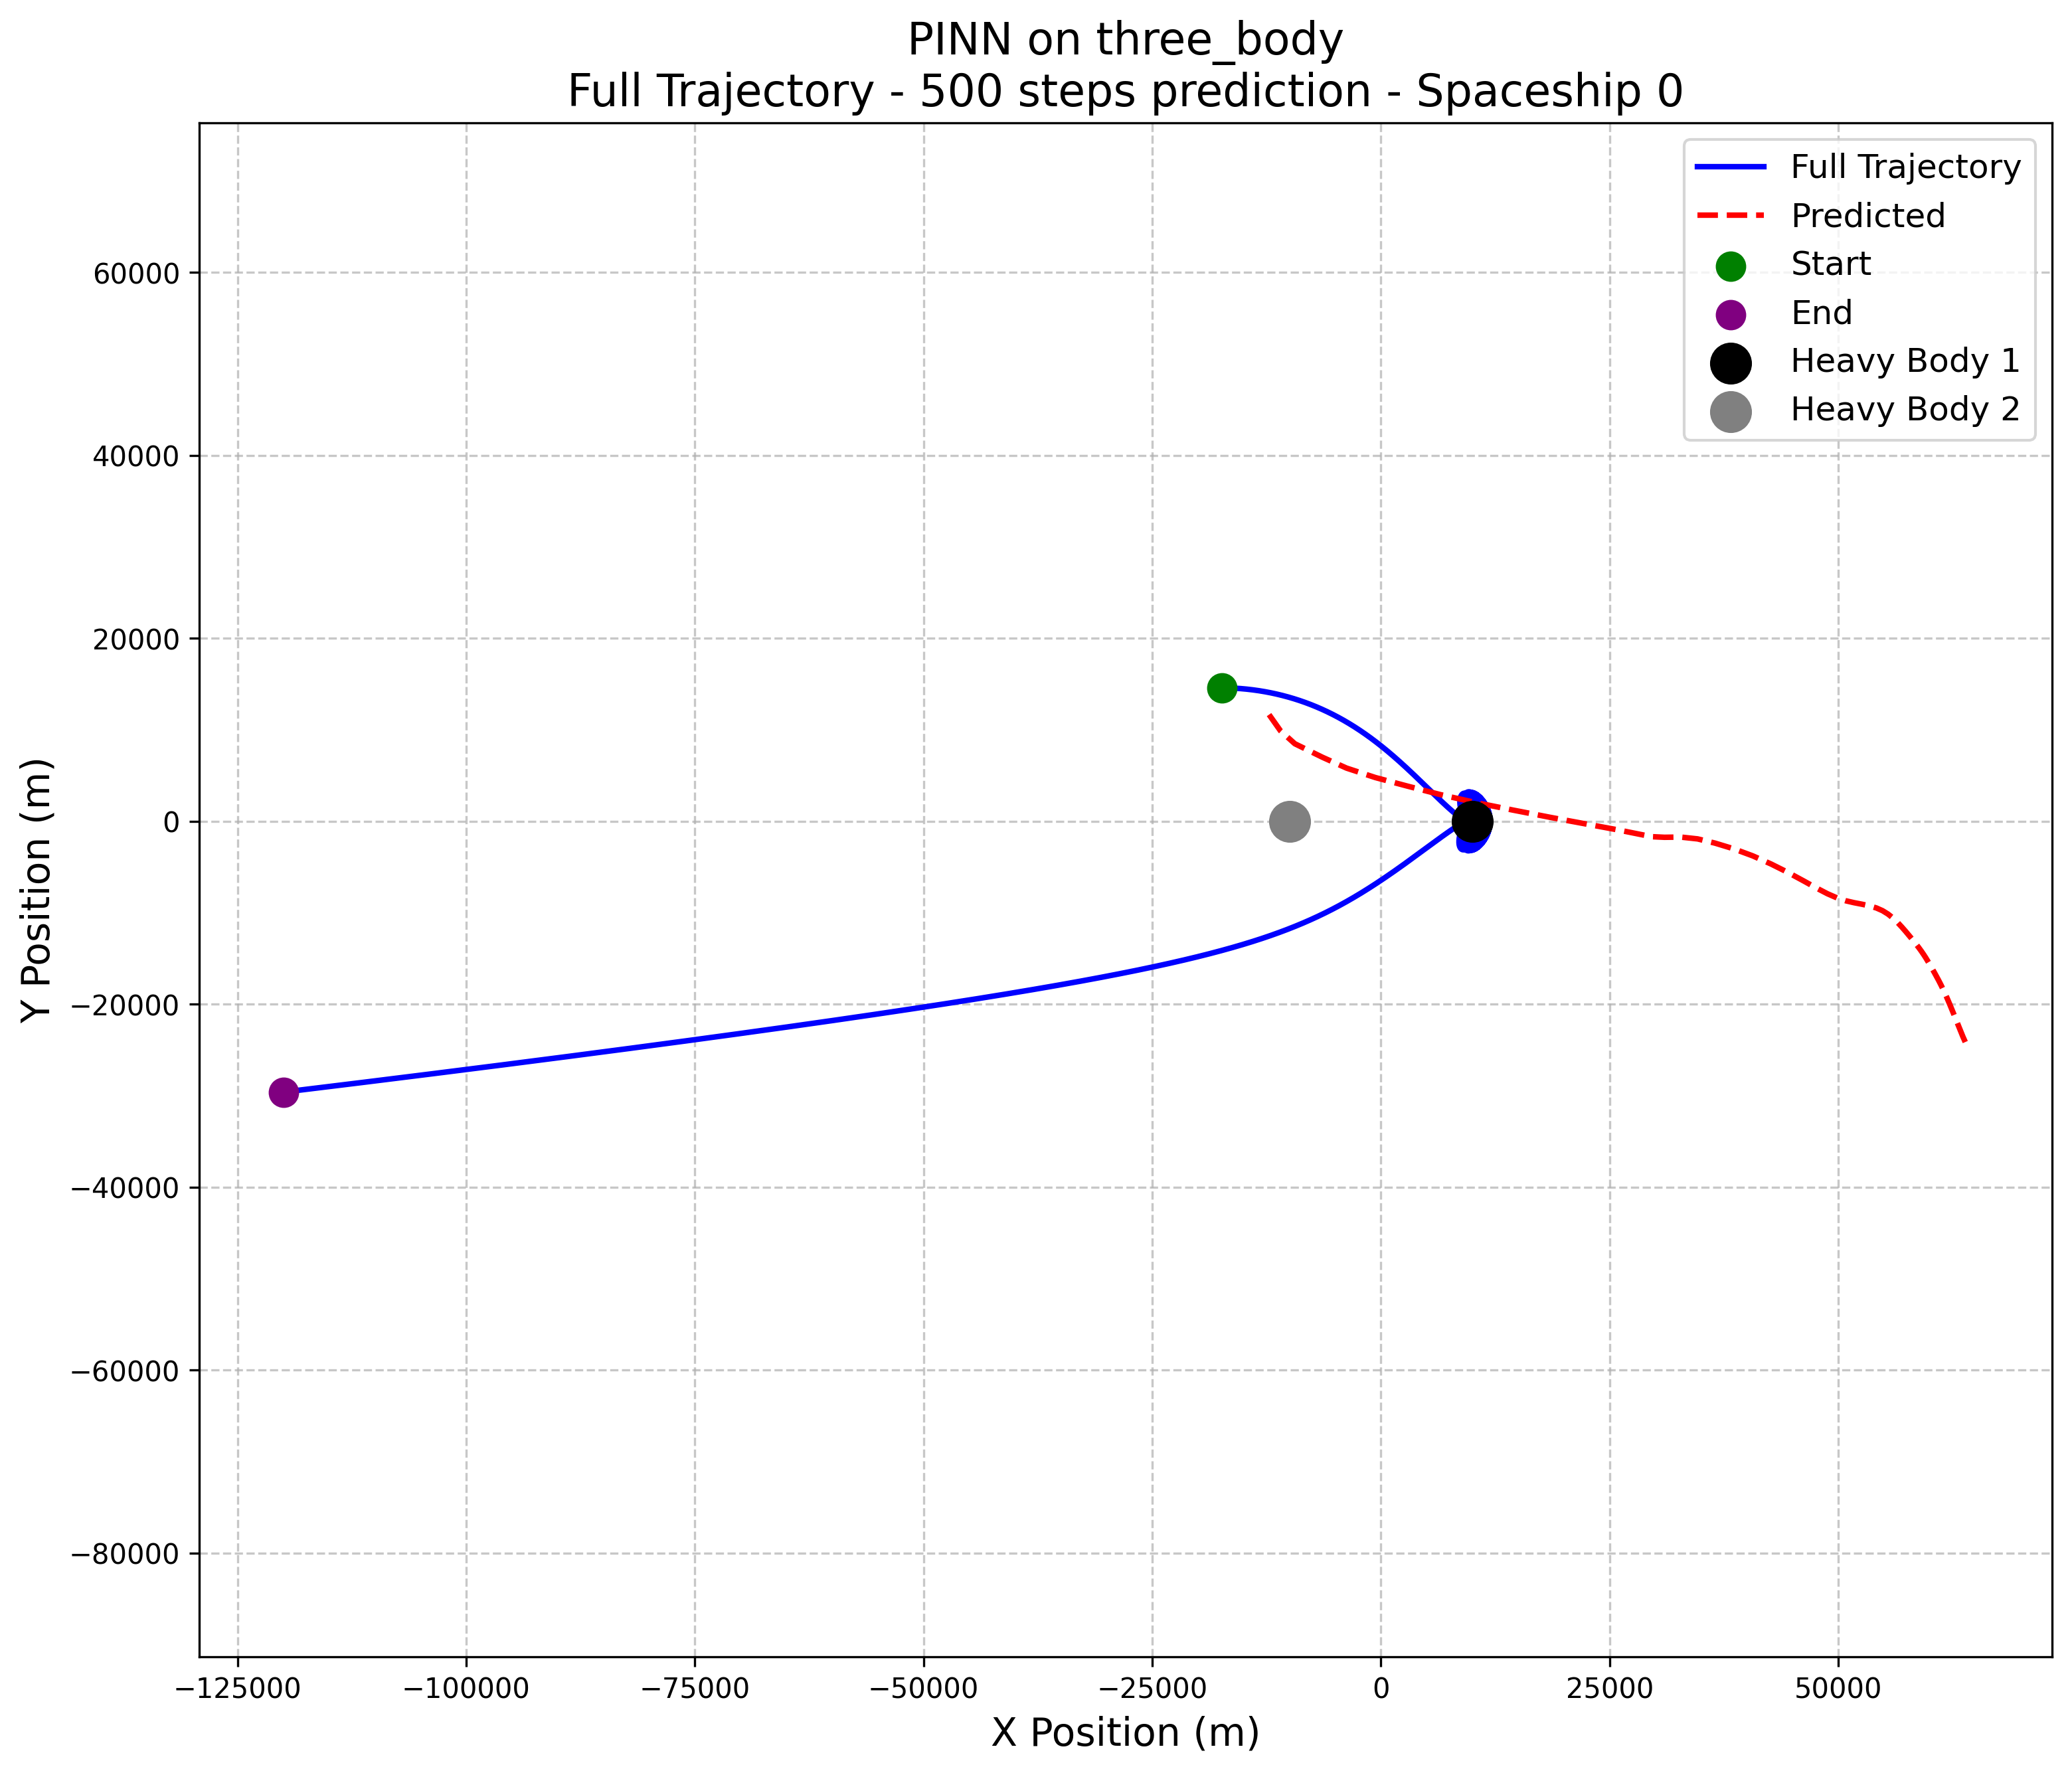
\includegraphics[width=0.27\textwidth]{../inference_results/val/PINN/three_body/500/full_trajectory_spaceship_0.png} &
      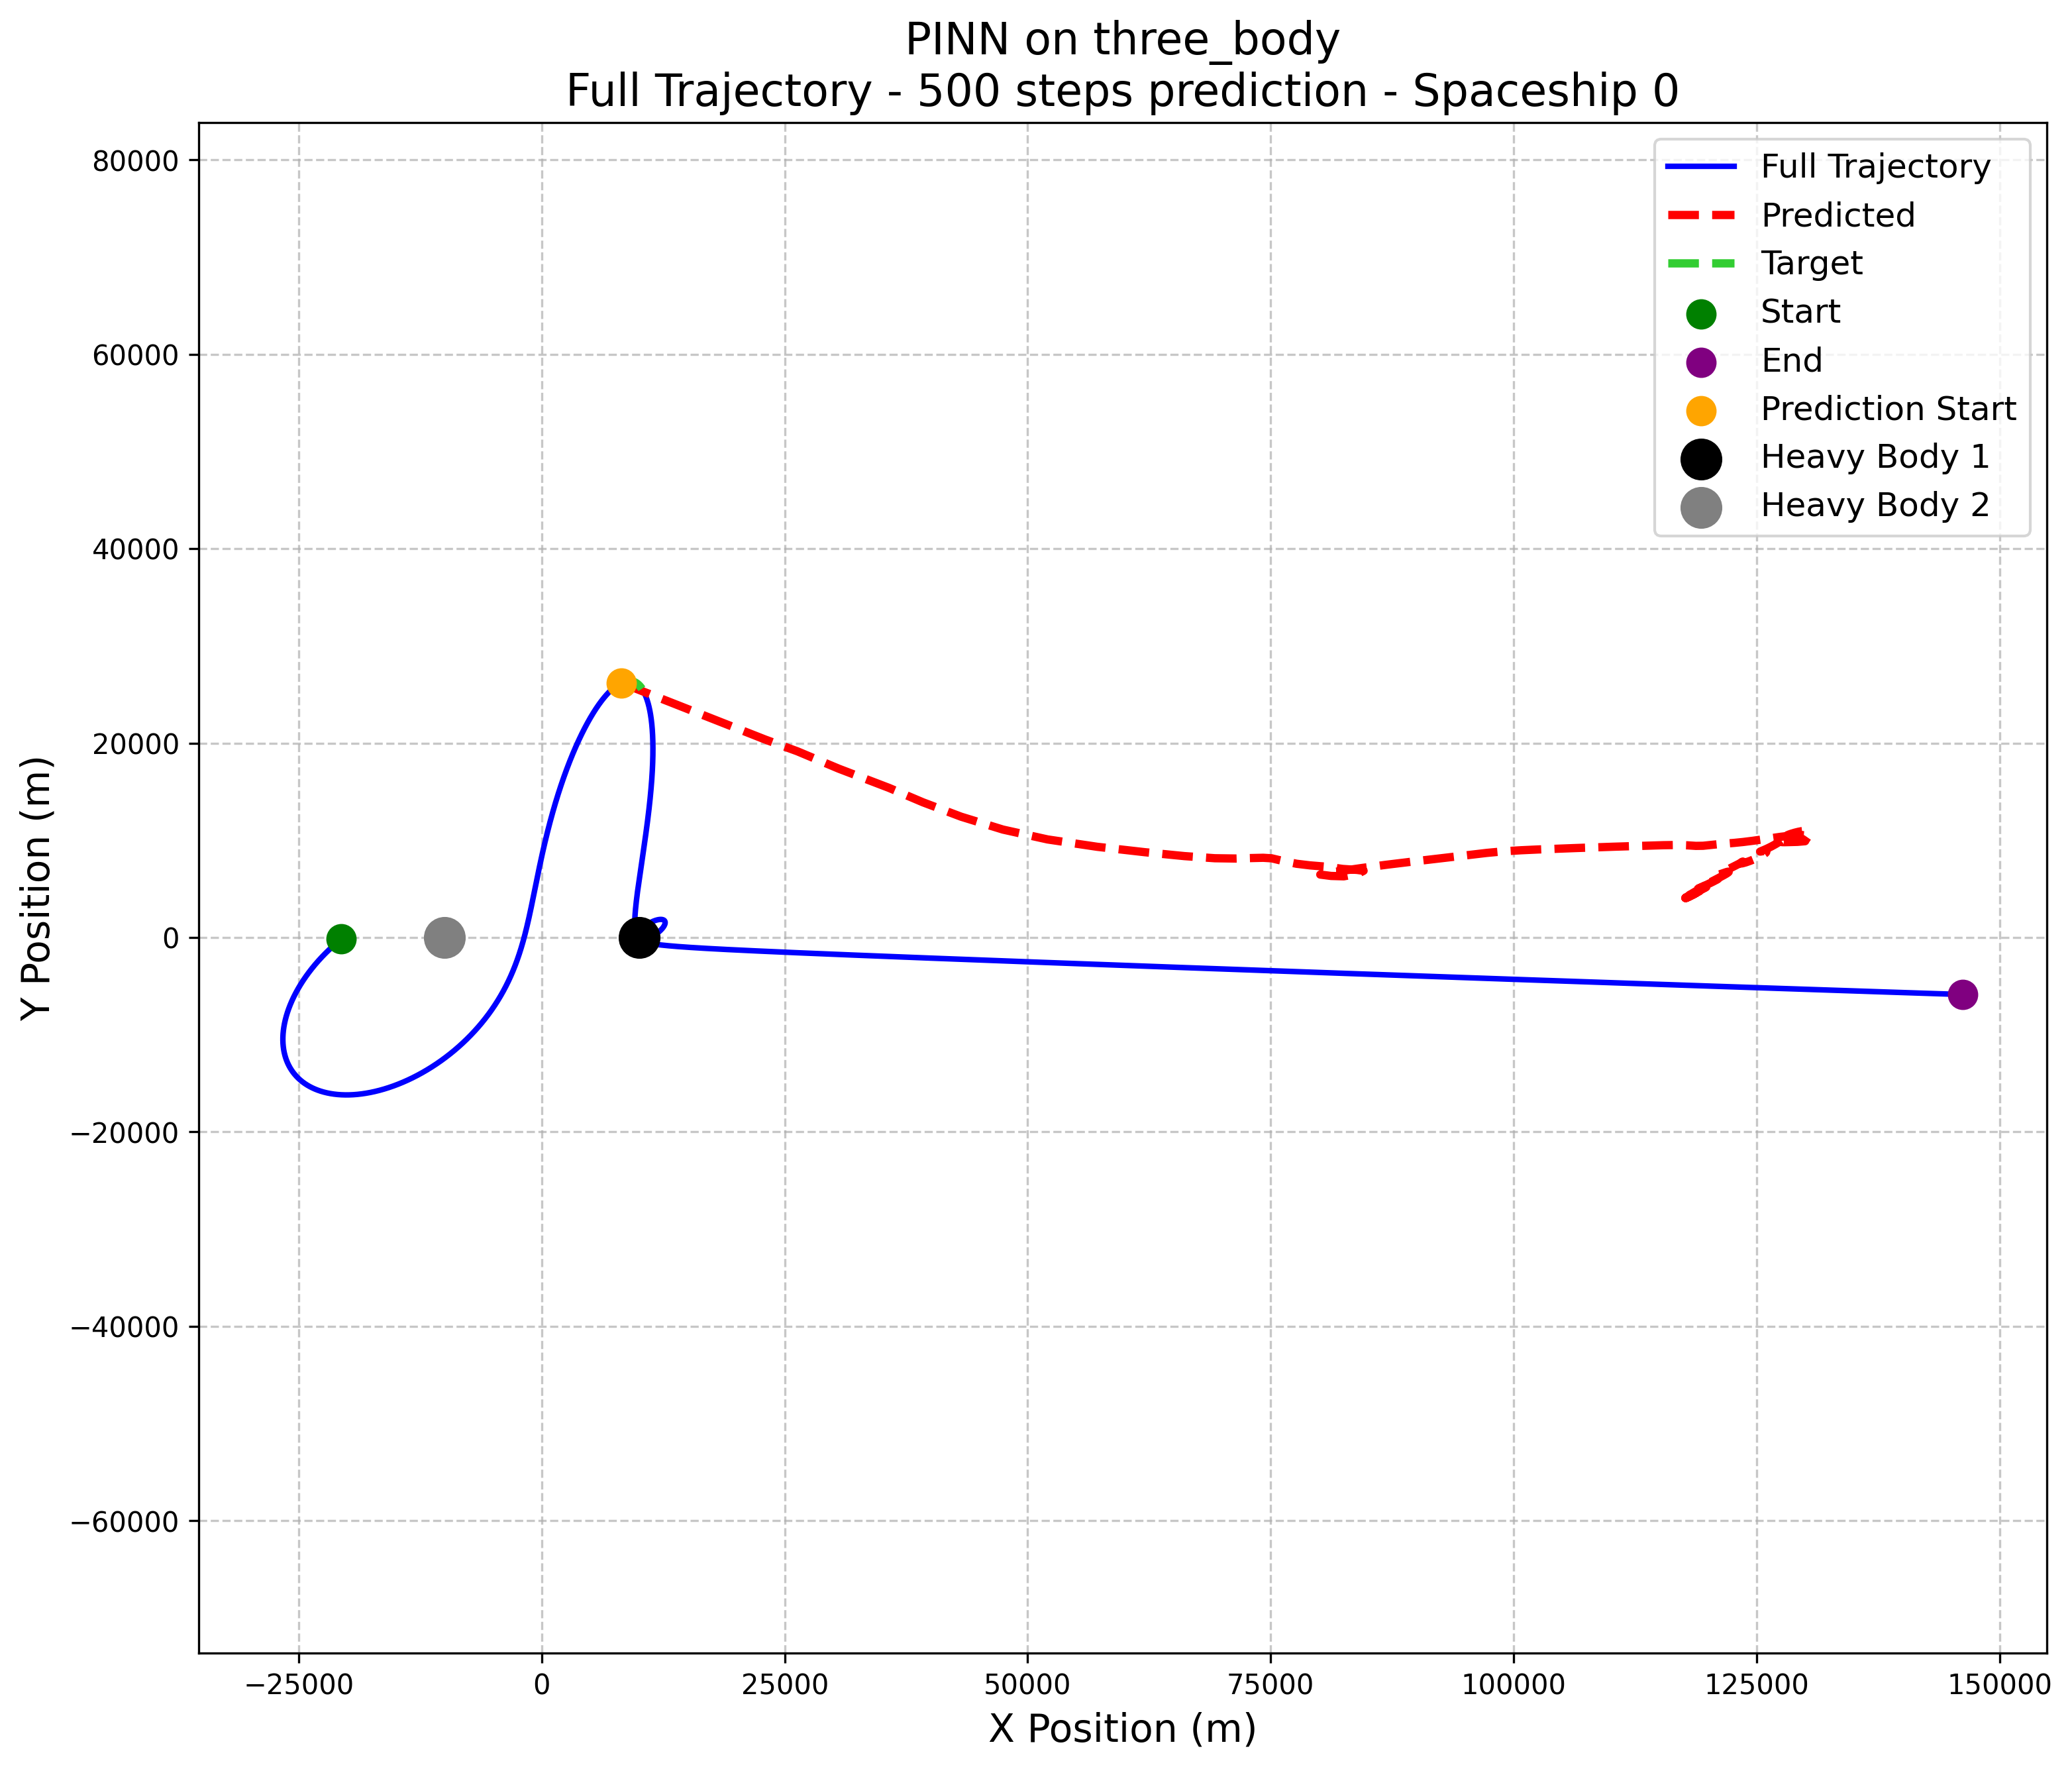
\includegraphics[width=0.27\textwidth]{../inference_results/test/PINN/three_body/500/full_trajectory_spaceship_0.png}
  \end{tabular}
\end{figure}
\end{document}

\section{Repository}
\label{sec:repository}
\begin{itemize}
  \item \textbf{checkpoints/}: Contains saved model states for different architectures and datasets
  \begin{itemize}
      \item Subfolders for LSTM, MLP, and PINN models
      \item Further subdivided by dataset types (three\_body, two\_body, two\_body\_force\_increased\_acceleration)
      \item Each subfolder contains model states (saved with Pytorch) for different folds (e.g., lstm\_fold0.pth, lstm\_fold1.pth, etc.)
  \end{itemize}

  \item \textbf{code/}: Main source code directory
  \begin{itemize}
      \item \texttt{data\_generation/}: Scripts for generating simulation data
      \item \texttt{inference/}: Code for running model inference and evaluation
      \item \texttt{training/}: Implementation of different model architectures and training procedures
      \begin{itemize}
          \item Separate subfolders for LSTM, MLP, and PINN models
          \item Each subfolder contains architecture, constants, and training scripts
      \end{itemize}
  \end{itemize}

  \item \textbf{datasets/}: Contains the generated datasets for different scenarios
  \begin{itemize}
      \item Subfolders for three\_body, two\_body, and two\_body\_force\_increased\_acceleration
      \item Each scenario has train, validation, and test data splits
      \item Training and validation data further divided into multiple folds for cross-validation
  \end{itemize}

  \item \textbf{images/}: Visualizations of trajectories and velocities for different scenarios
  \begin{itemize}
      \item Separate subfolders for each scenario (three\_body, two\_body, two\_body\_force\_increased\_acceleration)
      \item Contains plots of individual trajectories, velocities, and combined
  \end{itemize}

  \item \textbf{inference\_results/}: Stores the output from model inference and evaluation
  \begin{itemize}
      \item CSV files with aggregated results for each model and dataset combination
      \item \texttt{consolidated\_results.csv} summarizing all experiments, used in table \ref{tab:model_comprehensive_mse_compact}
      \item Subfolders containing detailed predictions and visualizations for each model, dataset, and prediction step combination
      \item Subfolder \texttt{sequence\_results} contains the actual predictions for each sequence length / model / dataset combination
  \end{itemize}

\end{itemize}
